\documentclass[a4paper,11pt,english]{report}
\usepackage{graphicx} % Required for inserting images
\usepackage{physics}
\usepackage{xcolor}
\usepackage{amsmath}
\usepackage{amsthm}
\usepackage{amssymb}
\usepackage[english]{babel}
\usepackage{derivative}
\usepackage{bbold}
\usepackage{algorithm}
\usepackage{algpseudocode}
\usepackage{epigraph}
\usepackage{geometry}
\usepackage{csquotes}
\geometry{margin=0.7in}
\usepackage{longtable}
\usepackage{tabularx}
\usepackage{ltablex}
\usepackage{pdflscape}
\usepackage[hidelinks,colorlinks=true,linkcolor=blue,citecolor=blue]{hyperref}
\usepackage{subcaption}
\usepackage{array} % For better table formatting

\newtheorem{definition}{Definition}[section]
\newtheorem{theorem}{Theorem}[section]
\newtheorem{remark}{Remark}[theorem]
\newtheorem{lemma}{Lemma}[theorem]
\newtheorem{corollary}{Corollary}[theorem]

\newenvironment{dedication}
  {
   \thispagestyle{empty}% no header and footer
   \vspace*{\stretch{1}}% some space at the top
   \itshape             % the text is in italics
   \raggedleft          % flush to the right margin
  }
  {\par % end the paragraph
   \vspace{\stretch{3}} % space at bottom is three times that at the top
   \clearpage           % finish off the page
  }

\usepackage{nomencl}
\setlength{\nomlabelwidth}{3.5cm}
\makenomenclature

\title{Simulation of Systems Governed by Non-Quadratic Hamiltonians in Heisenberg Formalism}
\author{Taha HAMMADIA}
\date{April - June 2024}


\usepackage[style=nature]{biblatex}
\addbibresource{biblio.bib}

\begin{document}
\newcommand{\timeDeriv}[1]{\dv{#1}{t}}
\newcommand{\ihbar}{\frac{1}{i \hbar}}
\newcommand{\floor}[1]{\left\lfloor #1 \right\rfloor}
\newcommand{\ceil}[1]{\left\lceil #1 \right\rceil}
\newcommand{\average}[1]{\left\langle #1 \right\rangle}
\newcommand{\cumulant}[2]{\left\langle #1;#2 \right\rangle_c}
\newcommand{\normOrd}[1]{:#1:}
\newcommand{\proj}[2]{\ket{#1}\bra{#2}}
\newcommand{\kronecher}[2]{\delta_{#1, #2}}
\newcommand{\weyl}[1]{\{#1\}_S}
\newcommand{\anticomm}[2]{\left\{#1, #2\right\}}
\newcommand{\Comm}[3]{\text{Comm}_{#1}\left(#2 | #3\right)}
\newcommand{\poly}[2]{\text{poly}_{#1}\left(#2\right)}
\newcommand{\texp}[1]{\mathcal{T}\exp{\int_{0}^t dt' #1(t')}}
\newcommand{\Texp}[1]{\mathcal{T}\exp{#1}}
\newcommand{\pr}[1]{\text{Pr}[#1]}
\newcommand{\LS}[1]{\mathcal{L}_S\left(#1\right)}
\newcommand{\LSS}[2]{\mathcal{L}^{(#1)}_S\left(#2\right)}
\newcommand{\heis}[1]{\left(#1\right)_H}
\newcommand{\algorithmautorefname}{Algorithm}

\begin{figure}
    \centering
    
\includegraphics[width=15cm]{Pics/Logo1.png}
\end{figure}
{\let\newpage\relax\maketitle}
\begin{center}
     Supervised by Danijela Marković (CNRS) and Elie Gouzien (Alice \& Bob)
\end{center}
\vfill
\begin{center}
     Laboratoire Albert Fert, CNRS, Thales, Université Paris-Saclay, Palaiseau, France
\end{center}
\vfill
\begin{center}
    \begin{figure}[h!]
    \centering
    
\includegraphics[width=15cm]{Pics/Logo2.png}
\end{figure}
\end{center}

\vfill

\begin{center}
    \begin{figure}[h!]
    \centering
    
\includegraphics[width=10cm]{Pics/Logo3.png}
\end{figure}
\end{center}

\begin{center}
    \begin{figure}[h!]
    \centering
    
\includegraphics[width=6.5cm]{Pics/logo_ab.pdf}
\end{figure}
\end{center}

\pagenumbering{roman}

\newpage
\clearpage
\addcontentsline{toc}{chapter}{Résumé / Abstract}
\chapter*{Abstract}
The development of quantum devices for quantum information and quantum neuromorphic computing leads to the necessity to simulate open bosonic systems. Such systems are characterized by the canonical bosonic commutation relations which have interesting properties that are derived. Solving the dynamics of open systems described by more than quadratic Hamiltonians, by unusual jump operators like two-photon loss or under an external drive is quite challenging. Attempts to simulate these systems \textit{via} the evolution of the density matrix, by imposing a cutoff in the Fock basis, are limited by its memory complexity which grows exponentially with the number of bosonic modes. This report undertakes part of the work by presenting the problem in a rigorous manner and leveraging the Heisenberg representation to propose and compare different methods of resolution that circumvent the memory complexity problem. These methods try to estimate the value of the moments, which describe the full dynamics. A great emphasis is put into writing correctly the Heisenberg representation for an open system. The complexities of the different methods will be evaluated. Furthermore, since the different methods are based on approximations, stability problems arise and need to be studied. We present a framework to study the stability of the numerical system and compare it for different cases between the different methods. Finally, analytical expressions are derived for some particular cases. Doing so allows to deepen the understanding of the resolution of differential equations on operators.
\paragraph{Keywords:} open bosonic systems, Heisenberg representation, quantum Langevin equation, mean field, cumulant, bosonic commutation relations, equation of evolution of operators, numerical stability, time evolution approximation


\newpage
\clearpage
\addcontentsline{toc}{chapter}{Dedication}
\chapter*{Dedication}

\begin{dedication}
    To my parents whose sacrifices cannot be enumerated.\\
    To my family who has always supported me.\\
    To my friends who shared the path with me.\\
    To my professors and tutors who guided me.\\
\end{dedication}

\newpage
\clearpage
\addcontentsline{toc}{chapter}{Acknowledgements}
\chapter*{Acknowledgements}
I am deeply indebted to the administration of the International Center for Fundamental Physics, in particular to the coordinators of the Master and to Médina Mahrez who plays a key role in the organization of the Master.  I would also to thank the SOIE of Ecole Polytechnique whose administrative work allowed for the required paperwork to be processed smoothly.

This endeavour would have been impossible without the help of my supervisors Dr.\@ Danijela Marković of the CNRS and Dr.\@ Elie Gouzien of Alice \& Bob. Their advice and directions were crucial for developing an understanding of the problem. My internship would not have been a success without their advice and knowledge. I would also like to thank Dr.\@ Yann Beaujeault-Taudiere for suggesting to use the Padé approximant. Thanks should also go to Julien Dudas for their insights on the application side of our project. I am also grateful to the Laboratoire Albert Fert administration, both from the CNRS and Thales side.

I am tremendously grateful to Thales Research and Technology Palaiseau who financed this project and who are a big contributor to the success of the Laboratoire Albert Fert.

Many thanks should go to my parents and family for their unabating support throughout the different stages of my life. Finally, thanks should go to the professors, students and Post-Doctoral Fellows I met during my internship, in particular to Julien Dudas, Théo Malas-Danzé, Julien Berthomier, Baptiste Carles and Clara Zimmermann.

\tableofcontents
\listoftables
\listoffigures

\newpage
\clearpage
\nomenclature{MF}{Mean field (MF)}
\nomenclature{$a, b, a_i\ldots$}{Bosonic annihilators}
\nomenclature{$a^\dagger, b^\dagger, a^\dagger_i\ldots$}{Bosonic creators}
\nomenclature{$H$}{Hamiltonian}
\nomenclature{$(\cdot)_H$}{Heisenberg representations}
\nomenclature{$(\cdot)_S$}{Schrödinger representations}
\nomenclature{$\commutator{\cdot}{\cdot}$}{Commutator}
\nomenclature{$\anticomm{\cdot}{\cdot}$}{Anti-commutator}
\nomenclature{$\kappa, \gamma\ldots$}{Rate of jump operator}
\nomenclature{$M(\Vec{z}, \Vec{z}^*)$}{Moment generating function (MGF)}
\nomenclature{$K(\Vec{z}, \Vec{z}^*)$}{Cumulant generating function (CGF)}
\nomenclature{$K(\Vec{z}, \Vec{z}^*)$}{Cumulant generating function (CGF)}
\nomenclature{$\poly{q}{a_1, \ldots, a_N; a^\dagger_1, \ldots, a^\dagger_N}$}{Polynomial of $a_1, \ldots, a_N; a^\dagger_1, \ldots, a^\dagger_N$ of degree less or equal to $q$}
\nomenclature{$L_n$}{Jump operator}
\nomenclature{$K_k$}{Kraus operator}
\nomenclature{$\Theta$}{Big theta symbol (asymptotically comparable)}
\nomenclature{$o$}{Small o symbol (asymptotically negligible)}
\nomenclature{$O$}{Big o symbol (asymptotically dominated)}
\nomenclature{$\sim$}{Equivalent}
\nomenclature{$\rho$}{Density matrix}
\nomenclature{$\average{\cdot}$}{Average}
\nomenclature{$C_{\cdot}$}{Cumulant}
\nomenclature{$p$}{Cut-off of the approximation}
\nomenclature{$\Comm{n}{A}{B}$}{Iterated commutator $\commutator{A}{\commutator{A}{\commutator{A}{\ldots B}}}$}
\nomenclature{$\tau_H$}{Degree of the Hamiltonian $H$ minus $2$, represents the non-linearity of $H$}
\nomenclature{$P(\beta, \beta^*)$}{$P-$distribution}
\nomenclature{$P(\beta, \beta^*)$}{$P-$distribution}
\nomenclature{$W(\beta, \beta^*)$}{Wigner function}
\nomenclature{$\mathcal{P}(n)$}{Set of partitions of $\{1, \ldots, n\}$}
\nomenclature{$\mathcal{L}$}{Stability matrix}
\nomenclature{$t_p[\alpha]$}{Time of validity}
\nomenclature{$B_n$}{Bell numbers}
\nomenclature{$\texp{A}$}{Time-ordered exponential}
\nomenclature{$w_X$}{Number of monomials in $X$}
\nomenclature{$M_{\max, i}$}{Cutoff in Fock space for mode $i$}
\nomenclature{$T$}{Length of the time interval}
\nomenclature{$m$}{Degree of the Hamiltonian}
\nomenclature{$(p, q)$}{Degrees of the numerator and denominator in Padé approximate}
\printnomenclature

\chapter*{Introduction}
    \pagenumbering{arabic}
    \addcontentsline{toc}{chapter}{Introduction}
    \epigraph{Let there be light}{\textit{Genesis 1:3}}
    The year 2025 marks the $100^{\text{th}}$ birthday of the formulation of the Heisenberg principle and the algebraic structure of quantum physics~\cite{history_quantum}. 2025 will be celebrated as the International Year of Quantum Science and Technology organized by the UNESCO~\cite{webpage_quantum_2025}. This quantum century has allowed humankind to develop technologies based on the understanding of the Universe provided by quantum physics ([classical] computers, telecommunications, medical imaging, nuclear energy, chemistry, metrology\ldots). Nowadays, a new application of quantum physics, which aims to leverage quantum information, is being developed: quantum computing.

Quantum computers aim to exploit the potential advantage provided by quantum information that is absent in classical information. Such an advantage can be formulated as the superposition principle~\cite{superposition_time}, the exponential size of the Hilbert space~\cite{schuld} or entanglement~\cite{aspect1982experimental}. Many objects have been explored for building quantum computers. Amongst them, we can cite: trapped ions~\cite{nature_atomic_qubits, compact_ion_trap, explo_quant}, cold atoms~\cite{Book-Lukacs} including Rydberg atoms~\cite{quantum_opti_rydberg}, diamond cavities~\cite{diamond}, supra-conducting circuits~\cite{google-supra, bbn-supra}\ldots This project focuses on light, which can be in the optical range or in the microwave range  (bosonic error correction in Alice \& Bob and quantum neuromorphic computing in Laboratoire Albert Fert).

The development of quantum computing devices based on light in all its forms, whether they are based on single photon sources~\cite{pascale_nature}, on linear optics~\cite{rawad_quandela}, on the generation of continuous states of light~\cite{review_xanadu} or on manipulating superposition of coherent states~\cite{elie_cat} has increased the hopes of seeing useful quantum computers in our lifetimes. Nevertheless, engineering such devices requires being able to simulate them beforehand. Since quantum computers are not mature enough to use them for simulation~\cite{feynman2018simulating}, it still needs to be done on classical computers. This becomes challenging as we approach applications where a quantum advantage is hoped for.

This project is part of the effort of simulating quantum devices based on bosons. This is important since many applications, like quantum machine learning and quantum neuromorphic computing~\cite{taha_quandela, markovic2020physics, Dudas2023-xx}, require to run the quantum device a considerable amount of times (for example once for each set of parameters to be tried). In particular, machine learning and neuromorphic tasks require using non-linearities to engineer, amongst others, powerful classification tools. Previously, this non-linearity was achieved \textit{via} measurements. However, current devices at Laboratoire Albert Fert can produce a Kerr effect. Even though analytical expressions can be found for self-Kerr and cross-Kerr (cf.\@ \autoref{app-analytic-exp}), adding non-diagonal terms makes the problem very challenging, thus the interest of this work. 

In this report, we study the evolution in the Heisenberg picture of bosonic modes evolving under some unitary evolution with some quantum jumps that simulate the interaction with a Markovian environment, or include the environment modes. We shall present some methods that aim at solving such systems. We start by presenting a overview of the problem and of the literature (cf.\@ \autoref{generalities-chapter}). Afterwards, we present our personal contribution (cf.\@ \autoref{main-chapter}). A great care will be taken to quantitatively compare the different methods (cf.\@ \autoref{sub-num-stab} and \autoref{comp-methds}). Additionally, we try to provide proofs for the different claims we make. In order not to hamper the reading of the report, the results and the proofs are demarcated clearly, allowing the hastened reader to skip them if needed. The report contains many appendices that clarify it and provide additional details. 

\chapter{Generalities and Review of the Literature} \label{generalities-chapter}
\epigraph{[The universe] cannot be read until we have learnt the language and become familiar with the characters in which it is written. It is written in mathematical language\ldots}{\textit{Galileo Galilei}}
    \section{Bosonic Commutation Relations}
    \subsection{Motivation}
Let us consider a system made of $N$ bosonic modes that are described using the annihilators $a_1, \ldots, a_N$ which follow the commutation relations

\begin{eqnarray}
    \commutator{a_i}{a^\dagger_j} &=& \delta_{i j},\\
    \commutator{a_i}{a_j} &=& 0.
\end{eqnarray}

As we shall see afterwards, in order to study the time evolution of $a_i$, we need to evaluate, among other things, $\commutator{a_i}{H}$, where $H$ is the Hamiltonian of the system. In general, $H$ can be written as a polynomial of the operators $a_1, \ldots, a_N$ and of $a^\dagger_1, \ldots, a^\dagger_N$. We introduce the notation

\begin{equation}
    H = \poly{m}{a_1, \ldots, a_N; a^\dagger_1, \ldots, a^\dagger_N},
\end{equation}
meaning that the degree of $H$ is less or equal to $m$ (in the sense that, for each term of $H$, the \textbf{sum} of the powers of different operators is \textbf{less or equal} to $m$). Therefore, we need to know the properties of commutation relations between polynomials of bosonic annihilators and creators.


\subsection{Properties}

\subsubsection{Commutator Algebra}

In this part, we recall some usual properties of the commutator~\cite{commuator_wiki}. The proofs are given in~\autoref{proof-basic-commutator}.

\begin{theorem} \label{basic_commutator}
    The commutator $\commutator{\cdot}{\cdot}$ satisfies the following properties
    \begin{enumerate}
        \item $\commutator{\cdot}{\cdot}$ is anti-symmetric under exchange of the arguments.
        \item $\commutator{\cdot}{\cdot}$ is bilinear (i.e.\@ linear in each variable).
        \item $\forall A, B, C,\  \commutator{A}{B C} = \commutator{A}{B} C + B \commutator{A}{C}$ and $\commutator{B C}{A} = \commutator{B}{A} C + B \commutator{C}{A}$.
    \end{enumerate}
\end{theorem}

The last result has an interesting corollary if we consider a bosonic annihilator $a$.

\begin{corollary}
    Let $a$ be a bosonic annihilator, for each $n \in \mathbb{N}$, $\commutator{a}{a^{\dagger n}} = n a^{\dagger (n-1)}$ and $\commutator{a^n}{a^\dagger} = n a^{(n-1)}$
\end{corollary}

\subsubsection{Degree of Commutator of Polynomials}

The goal of this part is to state the result~\autoref{th_deg_comm}. This result will be very important in analysing the differential systems to solve and will allow us to distinguish between linear and non-linear systems. Even though this result is mentioned in the literature~\cite{quesada_deg}, the proof could not be found in the literature we read. The proof in~\autoref{proof-th_deg_comm} is, at the best of our knowledge, original.

\begin{theorem} \label{th_deg_comm}
    Let $p, m \in \mathbb{N}$, we have
    \begin{equation}
        \commutator{\poly{p}{a_1, \ldots, a_N; a^\dagger_1, \ldots, a^\dagger_N}}{\poly{m}{a_1, \ldots, a_N; a^\dagger_1, \ldots, a^\dagger_N}} = \poly{p+m-2}{a_1, \ldots, a_N; a^\dagger_1, \ldots, a^\dagger_N}
    \end{equation}

    where $\poly{q}{a_1, \ldots, a_N; a^\dagger_1, \ldots, a^\dagger_N}$ designates any polynomial of degree $q$.
\end{theorem}

    \section{Quantum Dynamics}
    Let us consider a quantum system driven by the Hamiltonian $H$ and by the jump operators $L_n$~\cite{explo_quant} which represent the interaction of the system with its environment. Before considering the Heisenberg representation, it is useful to remind the results of the Schrodinger representation.
        \subsection{Schrödinger Representation - Density Matrix}
            \label{schro-pic}
            \subsubsection{Presentation of the Method}

In the Schrödinger picture, the dynamics of the system is described by the state of the system, the operators being time-independent. For a closed system, the axioms of quantum mechanics indicate that the system can be described by a time-dependent ket $\ket{\psi}$~\cite{principles_dirac}. For an open system interacting with the environment, the description needs to be modified. Indeed, the state is now described by a density operator $\rho_S(t)$ that allows for statistical mixtures of quantum states (the subscript $S$ stands for Schrödinger). The density operator is Hermitian, semi-positive and of trace equal to one. Its time evolution, under a Hamiltonian $H_S(t)$ and quantum jumps $L_n(t)$ is given by the master equation~\cite{explo_quant}.
\begin{equation} \label{master_eq}
    \timeDeriv{\rho_S(t)} = \ihbar \commutator{H_S(t)}{\rho_S(t)} + \frac{1}{2} \sum_{n} \left(2 L_n(t) \rho_S(t) L_n^\dagger(t) - \anticomm{L_n^\dagger(t) L_n(t)}{\rho}\right).
\end{equation}

In practice, solving the master equation~\autoref{master_eq} is done by truncating the Fock space, turning the operators into finite dimension matrices represented in the Fock basis. The obtained system is thus solved numerically. This method is implemented by the Python module \texttt{QuTip}~\cite{qutip} or \texttt{dynamiqs}~\cite{dynamiqs}.

\subsubsection{Performance}

The required dimension for each mode goes linearly with the \textbf{maximum} number of photons expected for the mode. In particular, the method fails to describe Hamiltonians that lead to an increase of the number of photons in time. More rigorously, let us denote $M_{\max, i}$ the maximal number of photons per mode. The memory complexity (cf.\@ \autoref{remind_comp} for the convention on the notation for complexity) is $\Theta\left(\prod_{i = 1}^N M_{\max, i}\right)$. In particular, we see that the space dimension grows \textbf{exponentially} with the number of modes (for each additional mode, the dimension of the Hilbert space is multiplied by the maximum number of photons considered in this mode). Therefore, this approach is inefficient for describing a large number of modes.
        \subsection{Heisenberg Representation} \label{intro-heis-rep}
            %We have seen in \ref{schro-pic} that solving the dynamics of the system in the Schrödinger picture requires a large memory complexity. This can be very limiting since matrix operations need to be done on this representation, leading to a large time complexity. In this part, we change the representation of the dynamics in the hope that these problems are solved.

In the Heisenberg representation, the dynamics are described by the evolution of the operators. This transformation is defined carefully in the following section.

\subsubsection{Reminders Concerning the Heisenberg Picture}

In this part, the subscript $S$ refers to the Schrödinger picture while the subscript $H$ refers to the Heisenberg picture.

\begin{definition}[Heisenberg Picture]
    The Heisenberg picture is defined as:
    \begin{equation} \label{heisenberg-pic}
        O_H(t) \equiv U_S^\dagger(t) O_S(t) U_S(t)
    \end{equation}
\end{definition}

The following theorem gives how do operators evolve in the Heisenberg picture:

\begin{theorem}
    Under the Hamiltonian $H_S(t)$, the time evolution of $O_H(t)$ is given by:

    \begin{equation}
        \timeDeriv{O_H}(t) = \ihbar \commutator{O_H(t)}{H_H(t)} + \left(\pdv{O_S}{t}(t)\right)_H
    \end{equation}

    where $H_H(t)$ and $\left(\pdv{O_S}{t}(t)\right)_H$ are given by Eq.~\ref{heisenberg-pic}.
\end{theorem}
\begin{proof}
    We write using \ref{heisenberg-pic}:
    \begin{equation}
        \timeDeriv{O_H}(t) = \timeDeriv{U_S^\dagger}(t) O_S(t) U_S(t) + U_S^\dagger(t) O_S(t) \timeDeriv{U_S}(t) + U_S^\dagger(t) \pdv{O_S}{t}(t) U_S(t)
    \end{equation}
    Knowing that: $\timeDeriv{U_S}(t) = \ihbar H_S(t) U_S(t)$, we find:
    \begin{equation}
        \timeDeriv{O_H}(t) = - \ihbar U_S^\dagger(t) H_S(t) O_S(t) U_S(t) + \ihbar U_S^\dagger(t) O_S(t) H_S(t) U_S(t) + \left(\pdv{O_S}{t}(t)\right)_H
    \end{equation}
    Introducing $\mathbb{1} = U_S(t) U_S^\dagger(t)$ for the two first terms, we identify:
    \begin{equation}
        \timeDeriv{O_H}(t) = - \ihbar H_H(t) O_H(t) + \ihbar O_H(t) H_H(t) + \left(\pdv{O_S}{t}(t)\right)_H
    \end{equation}
    which the result to show.
\end{proof}


 \begin{remark}
     Let $O_S(t) \equiv a_S(t) b_S(t)$ be an operator in the Schrödinger picture, its Heisenberg is given by:
     \begin{eqnarray}
         O_H(t) &=& U_S^\dagger(t) a_S(t) b_S(t) U_S(t)\nonumber\\
         &=& U_S^\dagger(t) a_S(t) U_S(t) \ U_S^\dagger(t) b_S(t) U_S(t)\nonumber\\
         &=& a_H(t) b_H(t)
     \end{eqnarray}
     This computation shows that if $O_S(t)$ is a polynomial of some operators, then $O_H(t)$ is the same polynomial of the Heisenberg representation of the aforementioned operators. In particular, the commutation relations can be computed by using the expression in the Schrödinger picture and then replacing the operators by their Heisenberg representation.

     In particular, the ladder operators satisfy the commutation relations $\commutator{a_i(t)}{a_j(t)} = 0$ and $\commutator{a_i(t)}{a^\dagger_j(t)} = \delta_{i j}$ when the evolution is \textbf{Unitary}. 
 \end{remark}


            We have seen in \autoref{schro-pic} that solving the dynamics of the system in the Schrödinger picture requires a large memory. This can be very limiting since matrix operations need to be done on this representation, leading to a large time complexity. In this part, we change the representation of the dynamics in the hope that these problems will be solved.

In the Heisenberg representation, the dynamics are described by the evolution of the operators and a time-independent density matrix. This transformation is defined carefully in this section.

\subsubsection{Reminders Concerning the Heisenberg Picture}

In this part, the subscript or superscript $S$ refers to the Schrödinger picture, while $H$ refers to the Heisenberg picture. The evolution of a quantum state is given by the Kraus operators $K_k$~\cite{explo_quant, green_bible}
\begin{equation}
    \rho_S(t) = \sum_{k} K^{(S)}_k(t) \rho(0) K^{(S) \dagger}_k(t),
\end{equation}
with the normalization condition $\sum_k K^{(S) \dagger}_k(t) K^{(S)}_k(t)  = \mathbb{1}$ and the sum $\sum_{k}$ being potentially uncountable. This condition ensures that the trace of $\rho_S(t)$ is preserved. The Heisenberg representation is defined as~\cite{stack_exch_prod}

\begin{definition}[Heisenberg Representation]
    The Heisenberg representation of an operator $O_S(t)$ (with explicit time-dependence) is given by:
    \begin{equation}
        O_H(t) \equiv \sum_k K^{(S) \dagger}_k(t) O_S(t) K^{(S)}_k(t).
    \end{equation}
The Heisenberg representation of a density matrix is given by $\rho_H(t) \equiv \rho_S(0)$ (time-independent).
\end{definition}

The definition of the Heisenberg picture comes from the fact that \textbf{the averages of observables should not depend on the representation}. This can be generalized to any operator $O$ by taking linear combinations of $\frac{O+O^\dagger}{2}$ and $\frac{O-O^\dagger}{2i}$ which are observable. The average of the operator $O_S(t)$ (i.e. with explicit time-dependence) is given by
\begin{eqnarray}
    \average{O_S}(t) &=& \Tr{\rho_S(t) O_S(t)} = \sum_k \Tr{K^{(S)}_k(t) \rho_S(0) K^{(S) \dagger}_k(t) O_S(t)} \nonumber\\
    &=& \sum_k \Tr{\rho_S(0) K^{(S) \dagger}_k(t) O_S(t) K^{(S)}_k(t)} \nonumber\\
    &=& \Tr{\rho_S(0) \sum_k K^{(S) \dagger}_k(t) O_S(t) K^{(S)}_k(t)}.
\end{eqnarray}

We observe that $(A + \lambda B)_H = A_H + \lambda B_H$ and $\left(O^\dagger\right)_H = \left(O_H\right)^\dagger$. However, it is quite important to observe that in general $(A B)_H \neq A_H B_H$ unless the sum over $k$ is on one element (i.e.\@ closed system). In fact,

\begin{eqnarray}
    A_H(t) B_H(t) &=& \sum_k \sum_l K^{(S) \dagger}_k(t) A_S K^{(S)}_k(t) K^{(S) \dagger}_l(t) B_S K^{(S)}_l(t)\\
    (A B)_H(t) &=& \sum_k K^{(S) \dagger}_k(t) A_S B_S K^{(S)}_k(t).
\end{eqnarray}

Furthermore, the average $\average{A B}(t)$ is associated to $(A B)_H(t)$.

The interest of the Heisenberg picture is to study the evolution of average of operators, allowing us to follow a smaller number of quantities than required for solving the master equation~\autoref{master_eq}. For this purpose, we need to write the equation of evolution of the operators.

\begin{theorem}[Evolution equation in the Heisenberg Picture] \label{eq_evo_heisen}
    Under the Hamiltonian $H_S(t)$ and jump operators $L_n(t)$, the time evolution of $O_H(t)$, with $O_S$ time-independent, is given by
    \begin{equation} \label{equa-evo_heisen}
        \timeDeriv{O_H} = \left(\ihbar \commutator{O_S}{H_S(t)} + \frac{1}{2} \sum_n \left(L^\dagger_n(t) \commutator{O_S}{L_n(t)}  - \commutator{O_S}{L^\dagger_n(t)} L_n(t) \right)\right)_H.
    \end{equation}
\end{theorem}

\begin{proof}
    The master equation is given by:
    \begin{equation}
        \timeDeriv{\rho_S(t)} = \ihbar \commutator{H_S(t)}{\rho_S(t)} + \frac{1}{2} \sum_{n} \left(2 L_n(t) \rho_S(t) L_n^\dagger(t) - \anticomm{L_n^\dagger(t) L_n(t)}{\rho_S(t)}\right).
    \end{equation}
    Taking the average for the time-independent operator $O_S$, we find:
    \begin{eqnarray}
        \timeDeriv{\Tr{\rho_S(t) O_S}} &=& \ihbar \Tr{\commutator{H_S(t)}{\rho_S(t)}  O_S} + \frac{1}{2} \sum_{n} \left(2 \Tr{L_n(t) \rho(t) L_n^\dagger(t) O_S} - \Tr{\anticomm{L_n^\dagger(t) L_n(t)}{\rho(t)} O_S }\right) \nonumber\\
        &=& \ihbar \Tr{H_S(t) \rho(t) O_S} - \ihbar \Tr{\rho(t) H_S(t)  O_S}\nonumber\\
        &+& \frac{1}{2} \sum_{n} \left(2 \Tr{\rho(t) L_n^\dagger(t) O_S L_n(t)} - \Tr{L_n^\dagger(t) L_n(t) \rho(t) O_S} - \Tr{\rho(t) L_n^\dagger(t) L_n(t) O_S}\right)\nonumber\\
        &=& \ihbar \average{\commutator{O_S}{H_S(t)}} + \frac{1}{2} \sum_{n} \left(2 \average{L_n^\dagger(t) O_S L_n(t)} - \average{O_S L_n^\dagger(t) L_n(t)} - \average{L_n^\dagger(t) L_n(t) O_S}\right)\nonumber
    \end{eqnarray}
    We observe that: $2 L_n^\dagger O_S L_n - O_S L_n^\dagger L_n - L_n^\dagger L_n O_S = L_n^\dagger \left(O_S L_n - L_n O_S\right) + \left(L_n^\dagger O_S - O_S L_n^\dagger\right) L_n = L_n^\dagger \commutator{O_S}{L_n} - \commutator{O_S}{L_n^\dagger} L_n$. Furthermore, since our computation does not depend on the initial state $\rho(0)$, we deduce that:
    \begin{equation}
        \timeDeriv{O_H} = \left(\ihbar \commutator{O_S}{H_S(t)} + \frac{1}{2} \sum_n \left( L^\dagger_n \commutator{O_S}{L_n}  - \commutator{O_S}{L^\dagger_n} L_n \right)\right)_H
    \end{equation}
\end{proof}

\begin{remark}
    \autoref{eq_evo_heisen} implies that the evolution of an operator in Heisenberg picture can be computed using the standard bosonic commutation relations, since $O_S$ is a constant in \autoref{eq_evo_heisen}. This is important since commutation relations are not conserved for $t > 0$ (to see this consider $H = \hbar \omega a^\dagger a$ with the jump operator $L = \sqrt{\kappa} a$ where $\commutator{a(t)}{a^\dagger(t)} = e^{-\kappa t}$, see \autoref{misc-quad-one-loss} for a proof).
\end{remark}

\begin{remark}
    \autoref{equa-evo_heisen} does not need to have a closed form in $O_H$. It can depend on the Heisenberg representation of other operators. This is the crux of the problem of solving non-quadratic Hamiltonians (cf.\@~\autoref{intro-MF}).
\end{remark}


\paragraph{Example where $(A B)_H \neq A_H B_H$:} This example is from~\cite{stack_exch_prod}. Consider $H = \hbar \omega a^\dagger a$ with jump operators $L_1 = \sqrt{\kappa} a$ (spontaneous emission) and $L_2 = \sqrt{\kappa} e^{-\frac{\beta \hbar \omega}{2}} a^\dagger$ (thermal excitation). We can show that $a(t) = e^{-i \omega t -\frac{\gamma t}{2}} a(0)$ with $\gamma \equiv \kappa (1-e^{-\beta \hbar \omega})$. Thus: $a^\dagger(t) a(t) = e^{-\gamma t} a^\dagger(0) a(0)$. However, by writing and solving the differential equation on $n(t) \equiv \left(a^\dagger a\right)(t)$, we find: $n(t) = e^{-\gamma t} (n(0) - n_\infty) + n_\infty$, with $n_\infty$ corresponding to the Bose-Einstein distribution $n_\infty \equiv \frac{1}{e^{\beta \hbar \omega}- 1}$. Indeed, $n(t)$ represents the population which can go to a nonzero value while $a^\dagger(t) a(t)$ is a correlation that decays towards zero. \autoref{multi-heisenberg-multi} presents a sufficient condition that ensures that $(A B)_H = A_H B_H$. Even though the result is in itself not very practical, proving it gives a better understanding of the Heisenberg representation for an open system that can be seen by writing the equations of evolution for $(A B)_H$ and $A_H B_H$.

\paragraph{Comment on Bosonic Commutation Relations:} Even though $a(t)$ does not satisfy bosonic commutation relations for an open system and thus does not describe a boson in general, we show in this part that bosonic commutation relations are preserved. More specifically:

\begin{theorem}[Preservation of Bosonic Commutation Relations] \label{comm-preservation}
    We have for any open or closed bosonic system:
    \begin{eqnarray}
        \left(\commutator{a_i}{a_j}\right)(t) &=& 0\\
        \left(\commutator{a_i}{a^\dagger_j}\right)(t) &=& \delta_{i j}
    \end{eqnarray}
\end{theorem}

\begin{proof}
    We show more generally that the Heisenberg representation of a scalar $\lambda$ is constant. This proves the desired result since canonical bosonic commutators are scalar. We have
    \begin{equation}
        \lambda_H(t) = \sum_k K^{(S) \dagger}_k(t) \lambda K^{(S)}_k(t) = \lambda \sum_k K^{(S) \dagger}_k(t) K^{(S)}_k(t) = \lambda,
    \end{equation}
    where we used the normalization condition $\sum_k K^{(S) \dagger}_k(t) K^{(S)}_k(t)  = \mathbb{1}$.
\end{proof}

\begin{corollary}
    In the case of a \textbf{closed} system, we can write:
    \begin{eqnarray}
        \commutator{a_i(t)}{a_j(t)} &=& 0\\
        \commutator{a_i(t)}{a^\dagger_j(t)} &=& \delta_{i j}
    \end{eqnarray}
    This shows that $a_i(t)$ describes a boson for a closed system.
\end{corollary}

\begin{remark}
    We expect that adding the external input $a_{\text{in}}(t)$ and keeping the output $a_{\text{out}}(t)$, as done in a quantum Langevin equation, leads to a closed system where $(A B)_H = A_H B_H$. So far, this was not proven formally.
\end{remark}


\subsubsection{Case of Time-Independent Hamiltonian without Jump Operators}

In the case of a time-independent Hamiltonian without jump operators (i.e.\@ closed system), the Schrödinger and Heisenberg pictures of the aforementioned Hamiltonian are the same.

\begin{theorem}[Time-Independent Hamiltonian for a Closed System]
    For time-independent $H_S$: $H_S = H_H$.
\end{theorem}

\begin{proof}
    For $H_S$ time-independent: $U_S(t) = e^{-i\frac{H_S t}{\hbar}}$, which commutes with $H_S$.
\end{proof}

\begin{corollary}
    If $H_S$ is time-independent for a closed system, then $H_H$ is time-independent.
\end{corollary}

In the following, we will be interested in the operators that are not explicitly time-dependant, such as polynomials of ladder operators.

\begin{theorem}
    For $H_S$ and $O_S$ time-independent for a closed system, the time-evolution of $O_H$ is given by
    \begin{equation}
        O_H(t) = e^{i\frac{H_H t}{\hbar}} O_H(0) e^{-i\frac{H_H t}{\hbar}}
    \end{equation}
\end{theorem}

\begin{proof}
    For $H_S$ and $O_S$ time-independent, the equation of evolution of $O_H$ is given by
    \begin{equation} \label{equa-diff-closed}
        \timeDeriv{O_H(t)} = \ihbar \commutator{O_H(t)}{H_H}
    \end{equation}

    Since $H_H$ is time-independent, the solution of the differential equation is $O_H(t) = e^{i\frac{H_H t}{\hbar}} O_H(0) e^{-i\frac{H_H t}{\hbar}}$. This can be proven by showing that the right hand side \textit{satisfies the same differential equation} and \textit{has the same initial condition}.
\end{proof}

For the following, we will consider that all the operators are in the Heisenberg picture and drop the subscript $H$. In order to compute $O(t)$ explicitly, we introduce the following quantity.

\begin{definition}[Composition of Commutators]
    We define the sequence of operators $\Comm{n}{H}{O}$ by
    \begin{eqnarray}
        \Comm{0}{H}{O} &=& O\\
        \forall n \in \mathbb{N}, \Comm{n+1}{H}{O} &=& \commutator{H}{\Comm{n}{H}{O}}
    \end{eqnarray}
    which formally defines $\commutator{H}{\commutator{H}{\ldots\commutator{H}{O}}}$.
\end{definition}

Using this definition, we can write the time evolution of $O(t)$:

\begin{theorem} 
    For $H$ time-independent, we have
    \begin{equation} \label{exact_tea_expansion}
        O(t) = \sum_{n = 0}^\infty \frac{1}{n!} \left(\frac{i t}{\hbar}\right)^n \Comm{n}{H}{O(0)}
    \end{equation}
\end{theorem}

\begin{proof}
    We introduce the linear operator: $\Lambda : X \mapsto \ihbar \commutator{X}{H}$ (right hand side of~\autoref{equa-diff-closed}). Let us consider the linear differential equation: $\timeDeriv{X}(t) = \Lambda(X(t))$. The solution of this differential equation is $X(t) = \exp{t \Lambda}(X(0)) \equiv \sum_{n = 0}^\infty \frac{t^n}{n!} \Lambda^{(n)}(X(0))$, where $\Lambda^{(n)}$ designates the composition $n$ times. This is just a re-writing of~\autoref{exact_tea_expansion}.
\end{proof}

\begin{remark}
    In \autoref{exact_tea_expansion}, we can take $H$ both in the Heisenberg and the Schrödinger representations. Since we are computing its commutators with $O(0)$, $H$ should be considered in the Schrödinger picture. In particular, since all the operators are in the Schrödinger picture, \textbf{we can use the canonical commutation relations}.
\end{remark}
        \subsection{Mean Field Methods (MF)} \label{intro-MF}
        \subsubsection{Equations on Moments / Cumulants}
            We recall that the advantage of the Heisenberg picture is that it allows to follow a small number of interesting quantities, which does not have to scale in an exponential fashion with the number of modes. These quantities can be followed by writing differential equations on moments (i.e.\@ averages on monomials of annihilators and creators) or on cumulants (defined in~\autoref{cumulant-method}).

Let $N$ denote the number of  bosonic modes. It will turn out that we will find the differential equations (on moments or cumulants) by taking the average of the Heisenberg equations for the monomials of $a_i$ and $a^\dagger_i$, which can be written as $\poly{p}{a_1, \ldots, a_N; a^\dagger_1, \ldots, a^\dagger_N}$. Let us consider the Hamiltonian $H = \poly{m}{a_1, \ldots, a_N; a^\dagger_1, \ldots, a^\dagger_N}$. If we limit ourselves to unitary evolution, we find

\begin{eqnarray}
    \timeDeriv{\average{\poly{p}{a_1, \ldots, a_N; a^\dagger_1, \ldots, a^\dagger_N}}} &=& \ihbar \average{\commutator{\poly{p}{a_1, \ldots, a_N; a^\dagger_1, \ldots, a^\dagger_N}}{H}} \nonumber\\
    &=& \average{\poly{p + m - 2}{a_1, \ldots, a_N; a^\dagger_1, \ldots, a^\dagger_N}}.
\end{eqnarray}

Therefore, writing a closed differential system with monomials of degree less or equal to $p$ is possible if and only if $m \le 2$, i.e.\@ in the case of a quadratic Hamiltonian~\cite{elie-these, Dudas2023-xx}. States produced by quadratic Hamiltonians (i.e.\@ Gaussian evolution) from vacuum are called Gaussian states~\cite{elie-these, quesada-fast-sum-Gauss}. They are characterized by a Gaussian Wigner distribution~\cite{explo_quant, quesada-fast-sum-Gauss, walls_milburn}. Knowing exactly the moments for a non-quadratic Hamiltonian requires solving \textit{an infinite number of Heisenberg equations}. Such an evolution is called non-Gaussian. Therefore, closing the system of equation on moments requires using an approximation that allows to express higher order moments as a function of lower order moments.

In general, there are $(2N+1)^p$ monomials containing at most $p$ annihilators and creators. However, using bosonic commutation relations, we can limit ourselves to normal order (i.e.\@ we limit ourselves to polynomials having creators at the left and annihilators to the right). The moments of degree less or equal to $p$ can be put in the form $\average{\left(\prod_{i = 1}^N a^{\dagger j_i}_i\right) \left(\prod_{i = 1}^N a^{k_i}_i\right)}$ with $\sum_{i=1}^N j_i+k_i \le p$. We might be interested in knowing the number of independent Heisenberg equations for moments of order $p$. Let $1 \le q \le p$ denote the total degree of a monomial. To count the number of monomials of degree $q$, we can consider $a_i$ and $a^\dagger_i$ as boxes where we can put $q$ balls. The corresponding combinatorics problem corresponds to choosing $q$ balls amongst $q$ balls and $2N-1$ separators (that separate between the boxes), i.e.\@ $\binom{2N+q-1}{q}$ choices. Summing over the different $q$'s, we get in total $\sum_{q=1}^p \binom{2N+q-1}{q}$ monomials to follow. We can further reduce the number of moments to follow by imposing $\sum_{i=1}^N j_i \le \sum_{i=1}^N k_i$, roughly by half (in the sense that the number of moments is $\sim \frac{1}{2} \sum_{q=1}^p \binom{2N+q-1}{q} = O(p^{2N})$ for $p \rightarrow \infty$, $N$ constant and $\sim \frac{(2 N)^p}{2 p!}$ for $N \rightarrow \infty$, $p$ constant; see \autoref{misc-nbr-eq} for a proof of these statements). In conclusion, fixing the order of the operators in the moments reduces significantly the number of moments to follow.

For the remaining, we define: $\tau_H \equiv m - 2$, the ``Hamiltonian non-linearity''. This number measures the degree of non-linearity of the Hamiltonian.

\paragraph{Interesting Corollary:} Let us consider the value of~\autoref{exact_tea_expansion} for $O = a_i$. Since each commutation with $H$ adds $\tau_H$ to the degree of the polynomial, we have:

\begin{equation}
    \Comm{n}{H}{a_i} = \poly{1 + n \tau_H}{a_1, \ldots, a_N; a^\dagger_1, \ldots, a^\dagger_N}
\end{equation}

In particular, for $\tau_H \ge 1$ (or $H$ non-quadratic), the annihilator $a_i(t)$ cannot be expressed in terms of a polynomial of a finite degree of the initial ladder operators. This should be contrasted with the quadratic case where $a_i(t)$ is linear in the ladder operators (i.e.\@ $a_i(t) = \sum_{j=1}^N \left(F_{ij}(t) a_j(t) +G_{ij}(t) a^\dagger_j(t)\right)$ as in~\cite{elie-these}). Thus, there is a \textbf{fundamental} physical difference between quadratic and non-quadratic Hamiltonians. Quadratic Hamiltonians lead to new bosonic quasi-particles~\cite{ginzburg1958theory} while non-quadratic Hamiltonians lead to excitations of any arbitrary number of the initial particles (i.e.\@ $a_i(t)$ can contain for example $a_i$, $a^2_i$\ldots).

        \subsubsection{Cumulant Method} \label{cumulant-method}
            This part is largely inspired by~\cite{khan2021physical} that introduces cumulants in normal order for a given state. In order to follow the evolution of initial cat states and other non-Gaussian states, we give a more general definition of cumulants. The problem of writing equations in terms of moments is that they increase exponentially as a function of the degree (at least for coherent states with $|\alpha| > 1$, see~\autoref{fig:Cumu_Mom_Coherent}). The idea is to introduce a quantity that decreases as a function of the degree. For many cases, cumultants can play such a role.
\begin{center}
    \begin{figure}[h!]
      \centering
      \includegraphics[width=0.9\linewidth]{Pics/Cumu_Mom_Coherent.pdf}
      \caption{Cumulants and moments for the state $\ket{1.5-1.25i}$ from \texttt{dynamiqs} \cite{dynamiqs} for the dimension $500$ in logarithm scale. The index $(j, k)$ corresponds to $\average{a^{\dagger j} a^k}$. $\average{a^{\dagger k} a^j}$ and $\average{a^{\dagger j} a^k}$ are complex-conjugate, thus we limit ourselves to $j \le k$. The indices are ranked in an increasing order of $j+k$. For each subset of fixed $j+k$, the lexicographic order is imposed.}
      \label{fig:Cumu_Mom_Coherent}
    \end{figure}
\end{center}

\paragraph{Moment Generating Function (MGF)} The \textbf{normal} characteristic function for the multi-mode case for the operator $X$ is defined as \cite{explo_quant, khan2021physical}
\begin{equation}
    M^{[X]}(\Vec{z}, \Vec{z}^*) \equiv \Tr{X \left(\prod_{k=1}^N e^{i z^*_k a^\dagger_k}\right) \left(\prod_{k=1}^N e^{i z_k a_k}\right)}.
\end{equation}

In~\cite{khan2021physical}, $X$ is a density operator. In our case, we only impose the normalization condition $\Tr{X} = 1$, ensuring that $M^{[X]}(\Vec{0}, \Vec{0}) = \Tr{X} = 1$. In  In particular, we can deduce directly the values of moments in normal order from the derivatives of $M^{[X]}(\Vec{z}, \Vec{z}^*)$

\begin{equation}
    \Tr{X\left(\prod_{k=1}^N a^{\dagger j_k}_k\right) \left(\prod_{k=1}^N a^{l_k}_k\right)} = \left[\prod_{k=1}^N \pdv[order = {j_k,l_k}]{}{(i z^*),(i z)}\right]M^{[X]}(\Vec{0}, \Vec{0}).
\end{equation}

This makes $M^{[X]}(\Vec{z}, \Vec{z}^*)$ the normal order moment generating function. While the symmetric characteristic function is associated with the Wigner function, $M^{[X]}(\Vec{z}, \Vec{z}^*)$ is associated with the Glauber–Sudarshan $P-$distribution defined as the complex Fourier transform of $M^{[X]}(\Vec{z}, \Vec{z}^*)$~\cite{walls_milburn, khan2021physical, wiki-quasi-prob, wiki-Glauber–Sudarshan},

\begin{equation}
    P^{[X]}(\Vec{\beta}, \Vec{\beta}^*) \equiv \frac{1}{\pi^{2 N}}\int \dd{z_1} \dd{z^*_1} \ldots \dd{z_N} \dd{z^*_N} M^{[X]}(\Vec{z}, \Vec{z}^*) e^{-i \Vec{\beta} . \Vec{z}} e^{-i \Vec{\beta}^* . \Vec{z}^*}.
\end{equation}

The $P-$distribution \cite{walls_milburn, khan2021physical} allows to represent a state $\rho$ on the coherent state basis:

\begin{equation}
    X = \int \dd{\beta_1} \dd{\beta^*_1} \ldots \dd{\beta_N} \dd{\beta^*_N} P^{[X]}(\Vec{\beta}, \Vec{\beta}^*) \ketbra{\Vec{\beta}}
\end{equation}

where $\ket{\Vec{\beta}} \equiv \ket{\beta_1} \otimes \ldots \otimes \ket{\beta_N}$.

\paragraph{Cumulant Generating Function (CGF)} The CGF is defined as: $K^{[X]}(\Vec{z}, \Vec{z}^*) \equiv \ln{M^{[X]}(\Vec{z}, \Vec{z}^*)}$. $K^{[X]}(\Vec{0}, \Vec{0}) = \ln{\Tr{X}} = 0$. $K^{[X]}(\Vec{z}, \Vec{z}^*)$ defines the cumulants as its derivatives at $(\Vec{0}, \Vec{0})$.

\begin{equation}
    C^{[X]}_{\left(\prod_{k=1}^N a^{\dagger j_k}_k\right) \left(\prod_{k=1}^N a^{l_k}_k\right)} \equiv \left[\prod_{k=1}^N \pdv[order = {j_k,l_k}]{}{(i z^*),(i z)}\right]K^{[X]}(\Vec{0}, \Vec{0}).
\end{equation}

It is possible to link moments and cumulants using the Faà di Bruno formula \cite{livre_faa, wiki-faa}. The lemma uses the notion of \textbf{partitions}. For a finite set $I$, $\mathcal{P}(I)$ denotes the \textbf{set} of \textbf{sets} of disjoint \textbf{subsets} of $I$ whose union is $I$. We denote $\mathcal{P}(n)$ as a short hand for $\mathcal{P}(\{1, \ldots, n\})$. For example, $\Big\{\{1, 2\}, \{3\}\Big\}$ and $\Big\{\{1, 2, 3\}\Big\}$ are partitions of $I = \{1, 2, 3\}$. More accurately, 
$$\mathcal{P}(3) = \Bigg\{\Big\{\{1\}, \{2\}, \{3\}\Big\}, \Big\{\{1, 2\}, \{3\}\Big\}, \Big\{\{1, 3\}, \{2\}\Big\}, \Big\{\{2, 3\}, \{1\}\Big\}, \Big\{\{1, 2, 3\}\Big\}\Bigg\}.$$ 
The number of elements of $\mathcal{P}(n)$ is given by the Bell number $B_n$ (cf.\@~\autoref{bell-append}), i.e.\@ $B_3 = 5$.

\begin{lemma}[Faà di Bruno formula] 
    Let $f$ and $g$ be differentiable $n-$times. We have:
    \begin{equation} \label{faa_form}
        \frac{\partial^n}{\partial x_1 ... \partial x_n} f(g) = \sum_{\pi \in \mathcal{P}(n)} f^{(|\pi|)}(g) \prod_{B \in \pi} \frac{\partial^{|B|} g}{\prod_{i \in B} \partial x_i}
    \end{equation}
    where $x_i$ can be any set of variables, with some potentially equal.
\end{lemma}

From this formula, we can deduce identities allowing us to express moments as a function of cumulants and cumulants as a function of moments:

\begin{theorem}[Passage from moments to cumulants and vice-versa in normal order] \label{th-m2c-c2m}
    Let $O_k$ be operators such that $\prod_{k=1}^n O_k \equiv O_1 \ldots O_N$ is written in the \textbf{normal} order. The following relations are true even if $\Tr{X} \neq 1$.
    \begin{eqnarray} \label{gen-m2c}
        C^{[X]}_{\prod_{k=1}^n O_k} &=& \sum_{\pi \in \mathcal{P}(n)} \frac{(-1)^{|\pi|-1} (|\pi|-1)!}{M^{[X]}(\Vec{0}, \Vec{0})^{|\pi|}} \prod_{B \in \pi} \Tr{X\prod_{i \in B} O_i}\\ \label{gen-c2m}
        \Tr{X\prod_{k=1}^n O_k} &=& \sum_{\pi \in \mathcal{P}(n)} e^{K^{[X]}(\Vec{0}, \Vec{0})} \prod_{B \in \pi} C^{[X]}_{\prod_{i \in B} O_i}
    \end{eqnarray}
    where $\prod_{i \in B} O_i$ is written in increasing order of $i$
\end{theorem}
\begin{proof}
    In this proof, we do \textbf{not} suppose that $\Tr{X} = 1$.
    
    For~\autoref{gen-m2c}, we use the relation $K^{[X]}(\Vec{z}, \Vec{z}^*) = \ln{M^{[X]}(\Vec{z}, \Vec{z}^*)}$. We use the Faà di Bruno formula~\autoref{faa_form} evaluated at $(\Vec{0}, \Vec{0})$. Further, we can show by induction that $\ln^{(n)}{x} = \frac{(-1)^{n-1} (n-1)!}{x^n}$, $n \ge 1$.

    For~\autoref{gen-c2m}, we use the relation $M^{[X]}(\Vec{z}, \Vec{z}^*) = \exp{K^{[X]}(\Vec{z}, \Vec{z}^*)}$. We use the Faà di Bruno formula~\autoref{faa_form} evaluated at $(\Vec{0}, \Vec{0})$. Further, $\exp^{(n)}{x} = \exp{x}$.
\end{proof}

\begin{corollary}
    Since we always impose that $\Tr{X} = 1$, the passage relations become:
    \begin{eqnarray} \label{m2c}
        C^{[X]}_{\prod_{k=1}^n O_k} &=& \sum_{\pi \in \mathcal{P}(n)} (-1)^{|\pi|-1} (|\pi|-1) \prod_{B \in \pi} \Tr{X\prod_{i \in B} O_i}\\
        \label{c2m}
        \Tr{X\prod_{k=1}^n O_k} &=& \sum_{\pi \in \mathcal{P}(n)} \prod_{B \in \pi} C^{[X]}_{\prod_{i \in B} O_i}
    \end{eqnarray}
    where $\prod_{i \in B} O_i$ is written in increasing order of $i$
\end{corollary}

\paragraph{Method (\texttt{truncated cumulants})} The method proposed in~\cite{khan2021physical} is to write differential equations on the \textit{cumulants}, which we will follow. However, it is possible to use cumulants to write differential equations on moments~\cite{quesada-fast-sum-Gauss, QuantumCumulants}. It is also possible to envision writing a closure relation using moments while writing differential equations on cumulants. This can be done by linking the higher degree moments to lower degree moments by setting the left hand side of~\autoref{m2c} to zero. The intuition behind writing the differential equations on cumulants is that for coherent states, cumulants are $0$ beyond the order $1$ and for Gaussian states cumulants are $0$ beyond the order $2$. Thus, at least for short times, we can suppose that cumulants beyond some order $p$ are $0$ as ``it takes time for them to be occupied''. This can be done by following the steps.

\begin{enumerate}
    \item Express the cumulants up to order $p$ in terms of moments using~\autoref{m2c}.
    \item Write the quantum Langevin equations for the moments which relate the time derivative of a moment to other moments.
    \item Write the time derivative of the cumulants in terms of moments by combining the two previous steps.
    \item Express the moments in terms of cumulants by replacing moments by cumulants using.~\autoref{c2m}. Impose that cumulants of order larger than $p$ are equal to $0$.
\end{enumerate}

One important limitation of the \texttt{truncated cumulants} is that the computation time is exponential in the cutoff $p$. The exponential time comes from summing on partitions in~\autoref{m2c} and~\autoref{c2m}, whose number (the Bell numbers) grows quasi-exponentially (see~\autoref{fig:Capture_Bell}). Writing the differential system on the cumulants becomes therefore cumbersome quite rapidly. See~\autoref{bell-append} for more information about Bell numbers.


\chapter{Solving Non-Quadratic Hamiltonians}  \label{main-chapter}
\epigraph{We must be clear that when it comes to atoms, language can be used only as in poetry.}{\textit{Niels Bohr}}
Unless stated otherwise, the results of this chapter are original to the best of our knowledge.
    \section{General Form of Quantum Langevin Equation} \label{find-langevin-gen}
        In~\autoref{2-langevin}, we present two derivations of the quantum Langevin equation which includes many photon loss, while including other jump operators that are represented by $L_n$. Many photon loss is described by the loss rate $\kappa_\nu$. The incoming field, denoted by $a_{\text{in}}(t)$, corresponds to an incoming propagating field. The first considers incoming propagating modes while the second considers a two cavity model.

\begin{equation} \label{generalized-langevin}
    \timeDeriv{a} = \ihbar \commutator{a}{H} + \frac{1}{2} \sum_n \left(L^\dagger_n \commutator{a}{L_n} - \commutator{a}{L^\dagger_n} L_n\right) - \sum_{\nu = 1}^\infty \nu a^{\dagger (\nu-1)} \left( \sqrt{\kappa_\nu}  a_{\text{in}}(t) + \frac{\kappa_\nu}{2}a^\nu \right)
\end{equation}

We observe that having higher than one photon loss is enough to lead to a nonlinear system (i.e. non-Gaussian dynamics). Furthermore, the term $- \nu \sqrt{\kappa_\nu} a^{\dagger (\nu-1)} a_{\text{in}}(t)$ couples the cavity field and the input field in a multiplicative manner.

\subsubsection{Examples}

Let us consider two examples:

\paragraph{One Photon Loss:} $\kappa_1 = \kappa$ and $\forall \nu \ge 2, \kappa_\nu = 0$. We get:

\begin{eqnarray}
    \timeDeriv{a} &=& \ihbar \commutator{a}{H} + \frac{1}{2} \sum_n \left(L^\dagger_n \commutator{a}{L_n} - \commutator{a}{L^\dagger_n} L_n\right) - \frac{\kappa}{2}a - \sqrt{\kappa}  a_{\text{in}}(t) 
\end{eqnarray}

which is the standard quantum Langevin equation.

\paragraph{Two Photon Loss:} $\kappa_2 = \kappa$ and $\forall \nu \neq 2, \kappa_\nu = 0$. We get:

\begin{eqnarray}
    \timeDeriv{a} &=& \ihbar \commutator{a}{H} + \frac{1}{2} \sum_n \left(L^\dagger_n \commutator{a}{L_n} - \commutator{a}{L^\dagger_n} L_n\right) -\kappa a^\dagger a^2 - 2 \sqrt{\kappa}  a^\dagger a_{\text{in}}(t)
\end{eqnarray}

\subsection{Sanity Check: Adding Jump Operators}

Alternatively, we could have obtain the quantum jump term of \ref{generalized-langevin} due to photon loss by adding the jump operators $\Tilde{L}_\nu \equiv \sqrt{\kappa_\nu} a^\nu$ to the Hamiltonian with the jump operators $L_n$. The additional term is indeed

\begin{equation}
    \frac{1}{2} \left(\Tilde{L}^\dagger_\nu \commutator{a}{\Tilde{L}_\nu} - \commutator{a}{\Tilde{L}^\dagger_\nu} \Tilde{L}_\nu\right) = - \frac{\kappa_\nu}{2} \commutator{a}{a^{\dagger \nu}} a^\nu = - \frac{\nu \kappa_\nu}{2} a^{\dagger (\nu - 1)} a^\nu.
\end{equation}
However, we cannot recover the term proportional to the input. This is because the input term $a_{\text{in}}(t)$ comes from considering the quantum state of the input field. This is not taken into account by the Heisenberg-Langevin equation, because it makes the density matrix of the Universe written as: $\rho_{\text{sys}} \otimes \rho_{\text{env}}$, and the environment is assumed to be Markovian.

\begin{remark}
    In the rest of this report, we do not consider the $a_{\text{in}}(t)$ term. If $a_{\text{in}}(t)$ describes a macroscopic coherent state, it can be simulated by adding a linear term to the Hamiltonian (for one-photon loss, we need to add the term $-i \hbar \sqrt{\kappa_1} \left(a^\dagger a_{\text{in}} - a^\dagger_{\text{in}} a\right)$, with $a_{\text{in}}$ a complex number). Otherwise, we do not know how to deal with time-dependent $a_{\text{in}}(t)$ in general~\cite{non-lin-green, paper-off-non-lin-green}.
\end{remark}

    \section{Mean Field (MF) Methods}
        As stated in the introduction, the goal of the MF method is to follow the moments that allow to rebuild all the desired quantities. The number of quantities to follow is expected to be much smaller than the number of variables of the density matrix. In this part, we present our contributions to the MF methods. As shown in~\autoref{app-all-moments}, many quantities can be found by knowing the moments. Additionally, MF methods can tackle time-dependent Hamiltonians and quantum jumps (cf.\@~\autoref{x-gate-ab}).
        \subsection{Summary of Other Methods}
            \subsubsection{Writing the Differential System}

The goal of this part is to follow the evolution of the moments of degree less or equal to $p$. We recall that the MF methods are based on approximating the equation of evolution of the moments. In particular, the equations of evolution for moments of degrees greater or equal to $p - \tau_H$ are approximated since the moments of degree larger than $p$ appear in them. Such a term can be for example $\average{a^{p+1}}$. Since we do not follow such a quantity, we need to be able to write it (in an approximate manner) in terms of moments of order less or equal to $p$. 

We have studied the following ways of approximating the moments of order larger than $p$.
\begin{enumerate}
    \item \texttt{Truncated cumulants}: this method is presented in~\autoref{cumulant-method}.
    \item \texttt{Divide in half}: this method is presented in~\autoref{divide-in-half}.
    \item \texttt{Minimum Cut}: this method is presented in~\autoref{min-cut}.
\end{enumerate}

Explicitly, we are interested in writing the moment $\average{\left(\prod_{l=1}^N a^{\dagger j_l}_l\right) \left(\prod_{l=1}^N a^{k_l}_l\right)}$ with $\sum_{l=1}^N j_l + k_l > p$.

\paragraph{\texttt{Divide in Half}} \label{divide-in-half}
The intuition behind this approach is that, if we take $p \ge \tau_H$, cutting the moment in two parts gives terms of degrees less or equal to $p$. For example, $\average{a^{p+1}} \mapsto \average{a^{\floor{\frac{p+1}{2}}}} \average{a^{\ceil{\frac{p+1}{2}}}}$.

More rigorously, this is done by representing the moment $\average{\left(\prod_{l=1}^N a^{\dagger j_l}_l\right) \left(\prod_{l=1}^N a^{k_l}_l\right)}$ by the tuple $T \equiv (j_1, ..., j_N, k_1, ..., k_N)$. The tuple can be manipulated by following~\autoref{alg:divide-in-half}. This algorithm is actually a heuristic as they are some cases that fail (for example $(3,~4,~4,~9)$ for $p=10$) Nevertheless, the method works for all the applications of interest.

\begin{algorithm}
\caption{Divide in Half Algorithm}\label{alg:divide-in-half}
\begin{algorithmic}
\Require T a tuple of length $2 N$, $p \in \mathbb{N}^*$ with $p \ge \tau_H$
\If{$\text{sum}(T) \le p$}
\State $L \gets [T]$
\Else
\State $i \gets$ \texttt{find$\_$idx}$(T, p)$ \Comment{\texttt{find$\_$idx} gives the smallest $i$ s.t. $\text{sum}(T[:i+1]) > p$}
\State $v\gets \min\left(p - \text{sum}(T[:i]), \ceil{\frac{T[i]}{2}}\right)$ \Comment{Divide in half here}
\State $L \gets \big[T[:i] + (v) + (0,)\times(2N-i-1), (0)\times i + (T[i] - v) + T[i+1:]\big]$
\EndIf
\State \Return L
\end{algorithmic}
\end{algorithm}

The reason behind trying to divide the ladder operator at position $i$ between the two resulting moments is to keep some correlation between them \textit{via} the aforementioned ladder operator. Furthermore, \texttt{divide in half} is intuitively \textit{expected} to be very accurate because the replacement is done by moments whose equation of evolution is correct. Thus the error is \textit{expected} to propagate to the second order.

\paragraph{\texttt{Minimum Cut}}  \label{min-cut}
The intuition behind this method is to divide the moment into the smallest possible number of chunks. This is done by taking chunks of size $p$ from $\average{\left(\prod_{l=1}^N a^{\dagger j_l}_l\right) \left(\prod_{l=1}^N a^{k_l}_l\right)}$ going from the left to the right. For example, $\average{a^{p+1}} \mapsto \average{a^{p}} \average{a}$.

More rigorously, like in~\autoref{divide-in-half}, this is done by representing the moment $\average{\left(\prod_{l=1}^N a^{\dagger j_l}_l\right) \left(\prod_{l=1}^N a^{k_l}_l\right)}$ by the tuple $T \equiv (j_1, ..., j_N, k_1, ..., k_N)$. The tuple is divided into chunks whose sum is equal to $p$. Usually, there will remain a last chunk whose sum is strictly less than $p$. The tuple can be manipulated by following~\autoref{alg:min-cut}. This algorithm is correct since each chunk has a sum less or equal to $p$.
\begin{algorithm}
\caption{Minimum Cut Algorithm}\label{alg:min-cut}
\begin{algorithmic}
\Require T a tuple of length $2 N$, $p \in \mathbb{N}^*$
\State $c \gets 0$, $i \gets 0$, $j \gets 0$, $L \gets []$
\While{$j < 2 N$}
\If{$c + T[j] < p$} \Comment{\texttt{Python} convention}
    \State $c \gets c + T[j]$, $j \gets j + 1$ \Comment{Accumulate ladder operators}
\Else \Comment{We have a chunk of degree $p$}
    \State $L \gets L + [(0)\times i + T[i:j] + (0)\times (2N-j-1)]$ \Comment{$(0)\times i = (0, 0, ..., 0)$ $i$ times}
    \State $T[j] \gets T[j] - p + \text{sum}(T[i:j])$ \Comment{Subtract the part already in a chunk}
    \State $c \gets 0$, $i \gets j$, $T[:j] \gets(0) \times j$
\EndIf
\EndWhile
\State $L \gets L + (0)\times i + T[i:]$ \Comment{The rest goes into a last chunk}
\State \Return L
\end{algorithmic}
\end{algorithm}

\subsubsection{Initial States}

For all the three methods, finding the initial condition can be done by finding the \textit{initial values of the moments}. We can show that this can be done for a large class of states. Indeed, we prove~\autoref{initial-general} in~\autoref{init-state-appendix} and give corollaries for a sum of coherent and of Fock states.

\begin{theorem}[Initial Value of Moments] \label{initial-general}
Let us consider the states $\{\ket{\phi[\xi]}\}_\xi$. We denote $a \ket{\phi[\xi]} = \lambda[\xi] \ket{\phi^{(1)}[\xi]}$, with $\ket{\phi^{(1)}[\xi]}$ is another state obtained after applying $a$ once on $\ket{\phi[\xi]}$. Let $\ket{\psi} = \sum_{\xi=1}^\chi c_\xi
\bigotimes_{i=1}^N \ket{\phi_i[\xi]}$. We have
\begin{equation}
    \mel{\psi}{\left(\prod_{l=1}^N a^{\dagger j_l}_l\right) \left(\prod_{l=1}^N a^{k_l}_l\right)}{\psi} = \sum_{\xi=1}^\chi \sum_{\zeta=1}^\chi c^*_\xi c_\zeta \prod_{l=1}^N \left(\prod_{\gamma = 0}^{j_l - 1} \lambda^{(\gamma)*}_l[\xi]\right) \left(\prod_{\kappa = 0}^{k_l - 1} \lambda^{(\kappa)}_l[\zeta]\right) \braket{\phi^{(j_l)}_l[\xi]}{\phi^{(k_l)}_{l}[\zeta]}
\end{equation}

where $\ket{\phi^{(k)}[\xi]}$ is the resulting state after applying $k$ times $a$ on $\ket{\phi[\xi]}$.
\end{theorem}

\paragraph{Numerical Implementation:} Even though~\autoref{initial-general} gives the expressions of the moments for states that are linear superpositions of states that we can handle, the resulting approximated differential system is very wrong since the state is very far from being Gaussian (see for example~\autoref{fig:CPictureCatCM}). Nevertheless, we have: $\rho = \sum_{\xi=1}^\chi \sum_{\zeta=1}^\chi c^*_\xi c_\zeta \bigotimes_{i=1}^N \ketbra{\phi_i[\zeta]}{\phi_i[\xi]}$. By linearity, the linear system can be solved by solving each projector $\bigotimes_{i=1}^N \frac{\ketbra{\phi_i[\zeta]}{\phi_i[\xi]}}{\braket{\phi_i[\xi]}{\phi_i[\zeta]}}$ (of trace one if $\braket{\phi_i[\xi]}{\phi_i[\zeta]} \neq 0$) independently (a similar idea is presented in~\cite{quesada-fast-sum-Gauss} for Gaussian evolution). A proof is given in~\autoref{proof-sum-gauss-non-lin}. This requires knowing the dot products $\braket{\phi_i[\xi]}{\phi_i[\zeta]}$. Indeed, if we consider a sum over coherent states, the projectors have zero cumulants for degrees larger or equal to $2$ (see fig. \ref{fig:PictureProj}).
\begin{center}
    \begin{figure}[h!]
      \centering
      \includegraphics[width=0.8\linewidth]{Pics/PictureCatCM.pdf}
      \caption{Cumulants and moments for the state $\propto \frac{\ket{3} + \ket{-3}}{\sqrt{2}}$ from \texttt{dynamiqs}~\cite{dynamiqs} for the dimension $500$ in logarithm scale. The index $(j, k)$ corresponds to $a^{\dagger j} a^k$. The index $(j, k)$ corresponds to $\average{a^{\dagger j} a^k}$. $\average{a^{\dagger k} a^j}$ and $\average{a^{\dagger j} a^k}$ are complex-conjugate, thus we limit ourselves to $j \le k$. For each subset of fixed $j+k$, the lexicographic order is imposed.}
      \label{fig:CPictureCatCM}
    \end{figure}
\end{center}

\begin{center}
    \begin{figure}[h!]
      \centering
      \includegraphics[width=0.9\linewidth]{Pics/PictureProj.pdf}
      \caption{Cumulants and moments for the projector $\frac{\ketbra{2}{1.5-3.7i}}{\braket{1.5-3.7i}{2}}$ using the exact numerical expression. The index $(j, k)$ corresponds to $\average{a^{\dagger j} a^k}$. The indices are ranked in an increasing order of $j+k$. For each subset of fixed $j+k$, the lexicographic order is imposed.}
      \label{fig:PictureProj}
    \end{figure}
\end{center}

To see this, let us consider the projector $\frac{\ketbra{\alpha}{\beta}}{\braket{\beta}{\alpha}}$. We have $M(z, z^*) = \Tr{\frac{\ketbra{\alpha}{\beta}}{\braket{\beta}{\alpha}} e^{i z^* a^\dagger} e^{i z a}} = \frac{\mel{\beta}{e^{i z^* a^\dagger} e^{i z a}}{\alpha}}{\braket{\beta}{\alpha}} = e^{i z^* \beta^*} e^{i z \alpha}$ (the expression is in normal order). Thus $\average{a^{\dagger j} a^k} = \beta^{* j} \alpha^k$. And $K(z, z^*) = i z^* \beta^* + i z \alpha$. Thus: $C_{a} = \alpha$, $C_{a^\dagger} = \beta^*$ and $C_{a^{\dagger j} a^k} = 0$ for $j + k \ge 2$.
        \subsection{Stability Analysis}
            Closing the system of differential equations requires applying an approximation to estimate the moments of order larger than $p$. On one hand, the approximation needs to be physically justified, which guarantees its correctness. On the other hand, it has to lead to a stable differential system under numerical errors. Indeed, since we treat the moments as independent variables, stability problems appear. This justifies studying the stability of the differential system under numerical errors. We start by introducing the following notions of local stability. The following notion is abstract and will be clarified afterwards.

\begin{definition}[General Notions of Local Stability]
    A system of differential equations can be linearized around any given point of the multi-dimensional space defined by the moments at a given time $t$. Depending on the real part of the eigenvalues $\{\lambda_i\}_i$ of the linearized differential system, we can classify the stability of the system at that specific point into three classes:
    \begin{enumerate}
        \item Stable: $\forall i, \Re{\lambda_i} < 0$
        \item Neutral: $\forall i, \Re{\lambda_i} \le 0$ and $\exists i, \Re{\lambda_i} = 0$
        \item Unstable: $\exists i, \Re{\lambda_i} > 0$
    \end{enumerate}
    The goal of this notion is to study whether the system amplifies numerical errors or not.
\end{definition}

\subsubsection{Introduction of $\mathcal{L}$}

We introduce the notation $f[j_1, \ldots, j_N, k_1, \ldots, k_N] \equiv \average{\left(\prod_{l=1}^N a^{\dagger j_l}_l\right) \left(\prod_{l=1}^N a^{k_l}_l\right)}$. We shall denote $\Vec{f}$ the vector containing $f[j_1, \ldots, j_N, k_1, \ldots, k_N]$'s. The order of the elements in the vector shall be fixed in the following manner. First, we put the elements such that $0 \le \sum_{l = 1}^N j_l \le \sum_{l = 1}^N k_l$ and $\sum_{l = 1}^N j_l + k_l \le p$ in a \textbf{lexicographic order}. Afterwards, we place in the same order the complex conjugate values (i.e.\@ $f[k_1, \ldots, k_N, j_1, \ldots, j_N] = f[j_1, \ldots, j_N, k_1, \ldots, k_N]^*$ will come in the same place in the second half than $f[j_1, \ldots, j_N, k_1, \ldots, k_N]$ in the first half). This ensures that $\Vec{f} = \begin{pmatrix}
    x\\
    x^*
\end{pmatrix}$. Further, the equation of evolution of $\Vec{f}$ that we obtain after applying the approximation can be written in all generality

\begin{equation}
    \timeDeriv{\Vec{f}} = \Vec{\mathcal{E}}\left(\Vec{f}\right).
\end{equation}
In order to study the stability, we consider a small deviation $\Vec{\epsilon}$ from a solution $\Vec{f_0}$. To linear order, $\Vec{\epsilon}$ satisfies the differential equation:

\begin{equation}
    \timeDeriv{\Vec{\epsilon}} = \nabla_{\Vec{f}} \Vec{\mathcal{E}}\left(\Vec{f_0}\right) \Vec{\epsilon}.
\end{equation}
For the following, we introduce the notation: $\mathcal{L} \equiv \nabla_{\Vec{f}} \Vec{\mathcal{E}}\left(\Vec{f_0}\right)$, such that:

\begin{equation}
    \mathcal{L}_{j_1, \ldots, j_N , k_1, \ldots, k_N; r_1, \ldots, r_N, s_1, \ldots, s_N} \equiv \pdv{\mathcal{E}_{j_1, \ldots, j_N, k_1, \ldots, k_N}}{{f[r_1, \ldots, r_N, s_1, \ldots, s_N]}}\left(\Vec{f_0}\right)
\end{equation}
By construction, the matrix $\mathcal{L}$ can be put in the form

\begin{equation} \label{general-form}
    \mathcal{L} = \begin{pmatrix}
        A & B\\
        B^* & A^*
    \end{pmatrix},
\end{equation}
with $A$ corresponding to $\sum_{l = 1}^N j_l \le \sum_{l = 1}^N k_l$ and $\sum_{l = 1}^N r_l \le \sum_{l = 1}^N s_l$ and $B$ corresponding to $\sum_{l = 1}^N j_l \le \sum_{l = 1}^N k_l$ and $\sum_{l = 1}^N r_l \ge \sum_{l = 1}^N s_l$. One remarks that some lines and columns are repeated (corresponding to $\sum_{l = 1}^N j_l = \sum_{l = 1}^N k_l$ and $\sum_{l = 1}^N r_l = \sum_{l = 1}^N s_l$). This is done to ensure that $\mathcal{L}$ has the form \ref{general-form}. Some additional properties of $\mathcal{L}$ are shown in~\autoref{ppties-L}.

\subsection{Numerical Tests} \label{sub-num-stab}

We compare the results for some quantum jumps: one-photon loss (cf.\@~\autoref{fig:CompStab1Loss}), two-photon loss (cf.\@~\autoref{fig:CompStab2Loss}) and dephasing (cf.\@~\autoref{fig:CompStabDeph}). We see that one-photon loss stabilizes all the methods. This is corroborated by~\autoref{fig:Eg_H_CrossKerr_1Loss}, \autoref{fig:Eg_H_CrossKerr_1Loss_stable}, \autoref{fig:Eg_H_Kerr_1Loss} and~\autoref{fig:Eg_H_Kerr_1Loss_stqble} in~\autoref{gene-other-plots}. Additionally, two-photon loss stabillizes \texttt{cumulant method} only, allowing us to conclude that the \texttt{cumulant method} is much more stable than the two others. Dephasing jump has no effect on the stability for all the methods.


\begin{figure}[h!]
    \centering
    \begin{subfigure}{0.32\linewidth}
        \centering
        \includegraphics[width=\linewidth]{Pics/H_0_and_losses_1_p_1_rule_trunc-cumul.pdf}
        \caption{Method \texttt{Truncated cumulants}}
        \label{fig:H_0_and_losses_1_p_1_rule_trunc-cumul}
    \end{subfigure}
    \hfill
    \begin{subfigure}{0.32\linewidth}
        \centering
        \includegraphics[width=\linewidth]{Pics/H_0_and_losses_1_p_1_rule_min-cut.pdf}
        \caption{Method \texttt{Minimum cut}}
        \label{fig:H_0_and_losses_1_p_1_rule_min-cut}
    \end{subfigure}
    \hfill
    \begin{subfigure}{0.32\linewidth}
        \centering
        \includegraphics[width=\linewidth]{Pics/H_0_and_losses_1_p_1_rule_smart_divide_in_half.pdf}
        \caption{Method \texttt{Divide in half}}
        \label{fig:H_0_and_losses_1_p_1_rule_smart_divide_in_half}
    \end{subfigure}
    \caption{Maximal value for the real part of the eigenvalues of the stability matrix $\mathcal{L}$ for quantum jump $\sqrt{\kappa} a$, coherent state $\ket{\alpha}$ and $p=1$.}
    \label{fig:CompStab1Loss}
\end{figure}

\begin{figure}[h!]
    \centering
    \begin{subfigure}{0.32\linewidth}
        \centering
        \includegraphics[width=\linewidth]{Pics/H_0_and_losses_2_p_2_rule_trunc-cumul.pdf}
        \caption{Method \texttt{Truncated cumulants}}
        \label{fig:H_0_and_losses_2_p_2_rule_trunc-cumul}
    \end{subfigure}
    \hfill
    \begin{subfigure}{0.32\linewidth}
        \centering
        \includegraphics[width=\linewidth]{Pics/H_0_and_losses_2_p_2_rule_min-cut.pdf}
        \caption{Method \texttt{Minimum cut}}
        \label{fig:H_0_and_losses_2_p_2_rule_min-cut}
    \end{subfigure}
    \hfill
    \begin{subfigure}{0.32\linewidth}
        \centering
        \includegraphics[width=\linewidth]{Pics/H_0_and_losses_2_p_2_rule_smart_divide_in_half.pdf}
        \caption{Method \texttt{Divide in half}}
        \label{fig:H_0_and_losses_2_p_2_rule_smart_divide_in_half}
    \end{subfigure}
    \caption{Maximal value for the real part of the eigenvalues of the stability matrix $\mathcal{L}$ for quantum jump $\sqrt{\kappa} a^2$, coherent state $\ket{\alpha}$ and $p=2$.}
    \label{fig:CompStab2Loss}
\end{figure}
    \section{Time Evolution Approximation (TEA)} \label{meth-tea}
        The hope of this method is to compute the time evolution in a symbolic manner, which can be done using \texttt{SymPy}~\cite{sympy}. The computed result is saved to solve the initial value problem for any initial value. The method allows to have changing parameters, which can be very useful for machine learning tasks~\cite{taha_quandela, markovic2020physics, Dudas2023-xx}.

The method corresponds to computing the expression $\sum_{n = 0}^\infty \frac{1}{n!} \left(\frac{i t}{\hbar}\right)^n \Comm{p}{H}{O(0)}$ in ~\autoref{exact_tea_expansion} using symbolic computation~\cite{sympy} up to some cut-off $p$. One advantage of this approach comparatively to the mean field approximations is that it ensures that the solution is correct for short times (in a rigorous manner). Furthermore, the divergence of the method is well-understood and very intuitive (the neglected terms become important). Additionally, this method has an advantage over the Schrödinger representation since the commutation relations are canonical. Such canonical relations do not exist with the density matrix. Finally, we access directly the correlations $\average{a^{\dagger j}(t) a^k(t)}$, and not the moments $\average{a^{\dagger j} a^k}(t)$.

\subsubsection{Can We Include Quantum Jumps?}
It turns out that we don't have an easy way to include quantum jumps for the TEA approximation. Nevertheless, we can do it in an \textbf{approximate} manner. For example, for one mode with $\nu-$photon loss, the term that needs to be added to the equation of evolution is: $- \nu \frac{\kappa_\nu}{2} a^{\dagger (\nu-1)} a^\nu$. This can be represented \textbf{approximately} by adding the term $-i \hbar \frac{\kappa_\nu}{2} a^{\dagger \nu} a^\nu$ to the Hamiltonian.

In~\autoref{comp-tea}, we show that the complexity of computing the commutators is given by

\begin{equation}
        C(p) = O\left(\sum_{n=0}^{p-1} w^{n+1}_H (1+m+n \tau_H)\right)
\end{equation}

where $w_H$ is the number of terms in $H$. Furthermore, it turns out (cf.\@~\autoref{proofs-time-val}) that the time of validity, i.e. the time where we expect the approximation to hold, grows at best in a linear fashion with $p$. Additionally, the proofs of~\autoref{proofs-time-val} allow us to extract the following pathological case.
\begin{corollary}
    We deduce from the proof that the Hamiltonians of the form $H = a^m + a^{\dagger m}$ for $m \ge 3$ are pathological in the sense that their validity time goes towards a constant. However, it turns out that TEA behaves better than \texttt{dynamiqs} \cite{dynamiqs} (cf.\@~\autoref{fig:H_pathos}).
\end{corollary}
\begin{figure}[h!]
    \centering
    \begin{subfigure}{0.49\linewidth}
        \centering
        \includegraphics[width=\linewidth]{Pics/Re_H_pathos.pdf}
        \caption{Real part}
        \label{fig:Re_H_pathos}
    \end{subfigure}
    \hfill
    \begin{subfigure}{0.49\linewidth}
        \centering
        \includegraphics[width=\linewidth]{Pics/Im_H_pathos.pdf}
        \caption{Imaginary part}
        \label{fig:Im_H_pathos}
    \end{subfigure}
    \caption{Evolution of $\average{a}(t)$ for $H = a^{\dagger 3} + a^3$ comparing different cut-offs $p$ and dimensions for \texttt{dynamiqs}~\cite{dynamiqs}.  Continuous line corresponds to the TEA for some cut-off while dashed line corresponds to \texttt{dynamiqs} for some dimension which corresponds to the value of $p$. $q = 0$ corresponds to not using the Padé approximate (cf.\@~\autoref{pade-approx-intro}).}
    \label{fig:H_pathos}
\end{figure}

\subsubsection{Padé Approximate} \label{pade-approx-intro}

The main takeaway of the previous part is that the time of validity of the TEA method increases at best linearly with the cut-off $p$ while taking an exponential cost in time for the number of monomials $w_H \ge 2$ in the Hamiltonian $H$ - in other words a little gain with a great cost. This prohibitive cost for improving accuracy can be partially tackled by using the Padé approximate~\cite{pade_mems, wiki-pade}.

Let us consider a function approximated by a Taylor expansion: $f(t) = \sum_{n=0}^P a_p t^n + O(t^{P+1})$. We know that the Taylor expansion diverges for $t \rightarrow \infty$. This means that the approximation becomes very wrong for functions that are bounded. Padé approximate leverages this observation and proposes to approximate $f(t)$ by a rational function instead of a polynomial, i.e.\@

\begin{equation}
    f(t) \approx \frac{\sum_{k=0}^p b_k t^k}{1 + \sum_{l=1}^q c_l t^l}.
\end{equation}
We observe that the Padé approximant is at least as good as Taylor expansion if the optimal value of the coefficient is chosen ($q = 0$ corresponds to Taylor expansion). Nevertheless, the numerical system can be ill-conditioned and cause numerical problems. In order to obtain the values of the coefficients $b_k$ and $c_l$, we solve the system

\begin{equation}
    \sum_{n=0}^N a_p t^n = \frac{\sum_{k=0}^p b_k t^k}{1 + \sum_{l=1}^q c_l t^l}.
\end{equation}
This can be done numerically using \texttt{scipy.interpolate.pade}~\cite{scipy}, with $p$ and $q$ hyper-parameters that need to be tuned. The only requirement is that $p+q \le P$ which ensures that the system has at least one solution. See~\autoref{fig:Pade} for examples of how the Padé approximant improves the result.

\begin{figure}[h!]
    \centering
    \begin{subfigure}{0.32\linewidth}
        \centering
        \includegraphics[width=\linewidth]{Pics/Pade_68_0.pdf}
        \caption{$(p, q) = (68, 0)$, i.e.\@~no Padé approximant}
        \label{fig:Pade_68_0}
    \end{subfigure}
    \hfill
    \begin{subfigure}{0.32\linewidth}
        \centering
        \includegraphics[width=\linewidth]{Pics/Pade_34_34.pdf}
        \caption{$(p, q) = (34, 34)$}
        \label{fig:Pade_34_34}
    \end{subfigure}
    \hfill
    \begin{subfigure}{0.32\linewidth}
        \centering
        \includegraphics[width=\linewidth]{Pics/Pade_17_17.pdf}
        \caption{$(p, q) = (17, 17)$}
        \label{fig:Pade_17_17}
    \end{subfigure}
    \caption{Evolution of $\Re{\average{a}(t)}$ using the TEA method improved using the Padé approximant for different values of $p$ and $q$, for  $H = a^\dagger b^\dagger b a$ and $L = \sqrt{0.1} a$. Continuous line corresponds to the TEA for some cut-off while dashed line corresponds to \texttt{dynamiqs}~\cite{dynamiqs} for some dimension.}
    \label{fig:Pade}
\end{figure}
    \section{Complexity of the Methods} \label{comp-methds}
        We compare the different methods by estimating their complexities in three different steps: writing the differential equations on scalar functions to solve, solving the differential system and evaluating the moments. We denote $T$ the length of the time interval of interest. Solving the differential equation has a time and memory complexity proportional to $T$. As a reminder, $N$ denotes the number of modes, $p$ the cut-off, $m$ the degree of the Hamiltonian, $w_H$ the number of terms in the Hamiltonian, $w_L$ the number of jump operators,  $M_{\max, i}$ the maximal number of photons for the mode $i$, $\chi$ the number of terms for the sum on Gaussian states, $B_p$ the $p^{\text{th}}$ Bell number, cf.\@~\autoref{bell-append}.

\subsection{Density Matrix Method}
We recall that the space dimension of the density matrix method is given by $\Theta\left(\prod_{i = 1}^N M_{\max, i}\right)$, which is exponential in the number of modes $N$. The three steps require manipulating matrices of size $\Theta\left(\prod_{i = 1}^N M_{\max, i}\right)$ \textit{via} multiplication, addition or inversion. Thus, the time complexity is proportional to a polynomial of $\Theta\left(\prod_{i = 1}^N M_{\max, i}\right)$.

\subsection{Usual MF}
This section refers to the methods \texttt{Divide in half} and \texttt{Minimum Cut}. The number of equations is $\sim \frac{1}{2} \sum_{q=1}^p \binom{2N+q-1}{q} = O((2N)^p)$. By using the bilinearity and product relation for the commutator, we can show that each equation has a time complexity $O((w_H + w_L) (p+m))$, where $w_H$ is the number of monomials in $H$ and $w_L$ is the number of jump operators. The memory complexity is $\sim \frac{1}{2} \sum_{q=1}^p \binom{2N+q-1}{q}$. The expressions can potentially been stored in an optimal manner. Solving the initial value problem requires using linear algebra polynomials, thus its time and memory complexities are given by $\Theta\left(T \text{poly}\left(\sum_{q=1}^p \binom{2N+q-1}{q}\right)\right)$. Retrieving the moments is straightforward since they are the values that are computed by solving the differential system. When the initial state is a sum over $\chi$ Gaussian states, we need to solve for each projector $\frac{\ketbra{\alpha_\xi}{\alpha_\zeta}}{\braket{\alpha_\zeta}{\alpha_\xi}}$ independently, thus leading to a factor $\chi^2$.

\subsection{Cumulant Method}
The cumulant method is similar to the usual MF methods. One important difference is time needed to convert moments to cumulants and vice-versa. This time scales as $B_p$, i.e.\@~the $p^{\text{th}}$ Bell number, see~\autoref{bell-append} for an introduction to Bell numbers. One important point is that $B_p$ grows exponentially with $p$. Writing differential equations on cumulants is usually done by converting differential equations on moments~\cite{khan2021physical}. Thus each term (a moment) needs to be converted into cumulants. For each equation, the number of terms is $O((w_H + w_L) (p+m))$. Furthermore, retrieving a moment requires converting back cumulants into moments, taking  a time proportional to $B_p$.

\subsection{Time Evolution Approximation}

For the TEA, the state is represented by the evolution of the annihilators $a_i(t)$. These states can be represented, up to the time of validity which can be expanded using Padé approximate, by the coefficients which can be written symbolically. Thus, their is no need to solve a differential system, solving the problem of stability. Additionally, retrieving a moment requires multiplying symbolic representations, which requires computing $\chi^2$ terms. The main limiting factor of this method is the time needed to compute the commutators. 

The results of this part are summarized in~\autoref{tab:comp-meths-1} and \autoref{tab:comp-meths-2}. Complexities are over-estimated (with $O$) for the sake of making the comparison easier. See \autoref{bell-append} for the asymptotic behavior of Bell numbers.

\begin{table}
    \centering
  \caption{Comparison of the complexities of the methods (Part 1). For definition of notations, see~\autoref{comp-methds}}
  \label{tab:comp-meths-1}
  \centering
  \makebox[\textwidth]{\begin{tabular}{|c|c|c|c|c|}
    \hline
    Step / Method & Density Matrix & Usual MF\\
    \hline
    Writing equations (time) & $\Theta\left(\text{poly}\left(\prod_{i = 1}^N M_{\max, i}\right)\right)$ & $O\left((w_H + w_L) (p+m) (2N)^p\right)$\\
    Writing equations (memory) & $\Theta\left(\prod_{i = 1}^N M_{\max, i}\right)$ & $O\left((2N)^p\right)$\\
    Solving equations (time) & $\Theta\left(T \text{poly}\left(\prod_{i = 1}^N M_{\max, i}\right)\right)$ & $\Theta\left(\chi^2 T \text{poly}\left((2N)^p\right)\right)$\\
    Solving equations (memory) & $\Theta\left(T \prod_{i = 1}^N M_{\max, i}\right)$ & $\Theta\left(\chi^2T \text{poly}\left((2N)^p\right)\right)$\\
    Retrieving a moment (time) & $\Theta\left(\text{poly}\left(\prod_{i = 1}^N M_{\max, i}\right)\right)$ & $O(\chi^2)$\\
    \hline
  \end{tabular}}
\end{table}

\begin{table}
    \centering
  \caption{Comparison of the complexities of the methods (Part 2). For definition of notations, see~\autoref{comp-methds}}
  \label{tab:comp-meths-2}
  \centering
  \makebox[\textwidth]{\begin{tabular}{|c|c|c|c|c|}
    \hline
    Step / Method &  Cumulant & TEA \\
    \hline
    Writing equations (time) & $O\left(B_p (w_H + w_L) (p+m) (2N)^p\right)$ & $O\left(N p w^{p}_H (m+p \tau_H)\right)$ \\
    Writing equations (memory) & $\sim \frac{1}{2} (2N)^p$ & $\Theta(N p + N p^2 \tau_H)$ \\
    Solving equations (time) & $\Theta\left(\chi^2 T \text{poly}\left((2N)^p\right)\right)$ & - \\
    Solving equations (memory) & $\Theta\left(\chi^2 T \text{poly}\left((2N)^p\right)\right)$ & - \\
    Retrieving a moment (time) & $\Theta(\chi^2 B_p)$ & $O(\chi^2 \text{poly}(p, \tau_H))$ \\
    \hline
  \end{tabular}}
\end{table}





\chapter{Conclusion} \label{cc-chapter}
\epigraph{The conclusion does not belong to the artist.}{\textit{Emile Zola}}
This concluding chapter starts by providing a summary of the different subjects presented in the report. Afterwards, it directs the reader towards the open questions that might be the subject of subsequent research.\\
\section{Summary of the Report}
We have studied how to solve open bosonic systems when finding exact analytical solutions is challenging, cf.\@~\autoref{app-analytic-exp}. After a brief overview of the literature (cf.\@~\autoref{generalities-chapter}), we showed how to write the quantum Langevin equation for many photon loss (cf.\@~\autoref{find-langevin-gen} and~\autoref{2-langevin}). Afterwards, we present our contribution to MF methods and introduced some tools to compare between them (cf.\@~\autoref{sub-num-stab} and~\autoref{comp-methds})(cf.\@~\autoref{app-squeeze}). We can study dynamics from states that can be expressed as a sum over low-cumulant states.  We also introduce the time evolution approximation (cf.\@~\autoref{meth-tea}) which allows to approximate the finite series of $a_i(t)$. A great care has been taken in comparing quantitatively the different methods and in proving the different statements. Appendices give some clarifications and details that could not be put in the report.

In particular, a summarized comparison between the methods is provided in \autoref{tab:summ-table}. The comparison highlights the strengths and weaknesses of the different methods. A key takeaway is that the choice of the method to apply depends on the particular needs of each case.
\section{Open questions}
Even though we had the opportunity to tackle many important and interesting questions during this project, many problems remain sadly unanswered. One such a question is the study of time-dependent inputs $a_{\text{in}}(t)$. The challenge arises from the difficulty of defining Green's functions for non-linear systems~\cite{non-lin-green, paper-off-non-lin-green}. This question is important if we desire to engineer more complex pulses than piece-wise constant inputs, even though piece-wise constant inputs are easier to optimize~\cite{emily}. It is possible that the mean methods can be used to solve the problem numerically. Furthermore, other theoretical questions remain open as highlighted in \autoref{tab:summ-table}. Even though, we have gained a greater understanding of the problem $(A B)_H \neq A_H B_H$ in \autoref{multi-heisenberg-multi}, we do not have yet a satisfying answer. A clear answer to this question will allow us to know when TEA is exact for an open system, for example. It will also tell us when correlations and moments are equal. 

Last but not least, these methods still need to be applied for experimental cases. 
\newpage
\clearpage
\addcontentsline{toc}{chapter}{Bibliography}
\printbibliography

\newpage
\clearpage
\appendix
\chapter{Additional Definitions} \label{def-app}
    \section{Notions of Complexity} \label{remind_comp}
        In this appendix, we introduce some notations for studying complexity. Since there are different notations~\cite{knuth, wiki-complexity}, we fix the one we will follow in this report.

\subsection{Presentation of the Problem}
When we are considering computational problems whose input size is given by $N$, we want to evaluate the needed resources for solving the problem using a given problem. For example, the computational time (in some time unit) or the memory size (in bits for example) might be of great importance.

Nevertheless, there is usually no need to know the exact value of the needed resources. Indeed, the exact value of the needed resources depends on the details of the machine. Thus, only the global evolution for $N$ going to infinity matters. For example, does the computation time go polynomialy with $N$? Does the memory requirement go exponentially with $N$?

\subsection{Notation Conventions}
We consider two functions $f(N)$ and $g(N)$ two functions. We want to compare their behavior at infinity. For this, we introduce the following definitions:

\begin{definition}[$o$ Notation]
    We say that $f(N) = o(g(N))$ when:
\begin{equation}
    \forall \epsilon > 0, \exists N_0 \in \mathbb{N}, \forall N \ge N_0, |f(N)| \le \epsilon |g(N)|
\end{equation}
\end{definition}

This means that $f(N)$ is negligible in front of $g(N)$.

\begin{definition}[$O$ Notation]
We say that $f(N) = O(g(N))$ when:
\begin{equation}
    \exists M > 0, \exists N_0 \in \mathbb{N}, \forall N \ge N_0, |f(N)| \le M |g(N)|
\end{equation}
\end{definition}

\begin{remark}
    It is quite important to understand that this notation does not mean that $f(N)$ and $g(N)$ become comparable when $N \rightarrow \infty$. For example, we can write: $N = O(e^N)$.
\end{remark}

If we want to say that $f(N)$ and $g(N)$ become comparable when $N \rightarrow \infty$, we use the $\Theta$ notation:
\begin{definition}[$\Theta$ notation]
    We say that $f(N) = \Theta(g(N))$ when:
\begin{equation}
    \exists M_1, M_2 > 0, \exists N_0 \in \mathbb{N}, \forall N \ge N_0, M_1 |g(N)| \le |f(N)| \le M_2 |g(N)|
\end{equation}
\end{definition}

In particular, we have:

\begin{theorem}
    We have: 
    \begin{enumerate}
        \item $f(N) = \Theta(g(N)) \iff g(N) = \Theta(f(N))$
        \item $f(N) = \Theta(g(N)) \implies f(N) = O(g(N))$
    \end{enumerate}
\end{theorem}

\begin{definition}[Equivalence]
    We say that $f(N) \sim g(N)$ ($f$ and $g$ are equivalent) when:
    \begin{equation}
        \lim_{N \rightarrow \infty} \frac{f(N)}{g(N)} = 1
    \end{equation}
\end{definition}

In particular, we have:

\begin{theorem}
    We have:
    \begin{enumerate}
        \item $f(N) \sim g(N) \iff g(N) \sim f(N)$
        \item $f(N) \sim g(N) \implies f(N) = \Theta(g(N))$
    \end{enumerate}
\end{theorem}
    \section{Bell Numbers} \label{bell-append}
        Bell numbers are a notion of combinatorics. It is \textbf{not} related to the famous Bell inequality in quantum physics. $B_n$ counts the number of partitions in a set $I$ of size $n$~\cite{knuth, OEIS-Bell}, i.e.\@~the number of sets of disjoint subsets of $I$ whose union is $I$. For example, $\{\{1, 2\}, \{3\}\}$ and $\{\{1, 2, 3\}\}$ are partitions of $I = \{1, 2, 3\}$.

Bell numbers are given by~\autoref{yoshi} which is due to Yoshisuke Matsunaga from the Japanese Edo era~\cite{knuth}.

\begin{theorem}[Yoshisuke Matsunaga] \label{yoshi}
    \begin{equation}
        B_{n+1} = \sum_{k=0}^n \binom{n}{k} B_k
    \end{equation}
\end{theorem}

For the purpose of analysing the complexity of the \texttt{truncated cumulants}(cf.\@~\ref{cumulant-method}), we need to estimate the asymptotic behavior of $B_n$. We use the result of de Bruijn~\cite{deBruijn}.


\begin{theorem}[De Bruijn]
    \begin{equation}
        \frac{\ln{B_n}}{n} = \ln{n} - \ln{\ln{n}} - 1 + o(1)
    \end{equation}
\end{theorem}

In a hand-waving approach, we could say that $B_n$ "behaves" as $n^n$, which signifies an exponential growth. Indeed, this can be seen in the plot~\autoref{fig:Capture_Bell} from~\cite{Graph-Bell}.

\begin{center}
    \begin{figure}[h!]
      \centering
      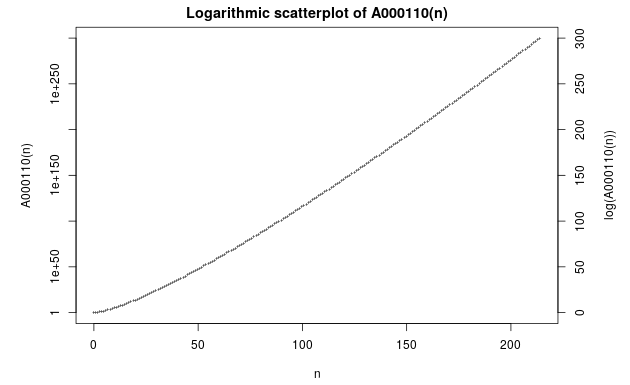
\includegraphics[width=0.6\linewidth]{Pics/Capture_Bell.PNG}
      \caption{Plot of Bell numbers from the OEIS \cite{Graph-Bell} in $\log_{10}$ scale}
      \label{fig:Capture_Bell}
    \end{figure}
\end{center}
        
\chapter{Sufficient Condition for Multiplicity of Heisenberg Representation} \label{multi-heisenberg-multi}
    This result is motivated by the fact that being able to write $(A B)_H = A_H B_H$ allows to solve many problems. In particular, we could solve analytically (cf.\@~\autoref{app-analytic-exp}) many problems if it were the case.

"Multiplicity of the Heisenberg representation" refers to the fact that $(A B)_H = A_H B_H$. This appendix is presented in a way that mimics the reasoning that we followed. The appendix gives a good reason why the Heisenberg representation is non-multiplicative.

In this part, we find a sufficient condition for having $(A B)_H = A_H B_H$. To the best of our knowledge, this result is original. We limit ourselves to a time-independent Hamiltonian $H_S$ and to quantum jumps $\{L_\mu\}_\mu$. Beforehand, we introduce the notation
\begin{equation}
    \LS{A} \equiv \ihbar \commutator{A}{H_S} + \frac{1}{2} \sum_\mu \left( L^\dagger_\mu \commutator{A}{L_\mu}  - \commutator{A}{L^\dagger_\mu} L_\mu \right)
\end{equation}

which corresponds to the right hand side of the equation in~\autoref{eq_evo_heisen} before taking the Heisenberg representation, i.e.\@~$\timeDeriv{A_H} = \heis{\LS{A}}$.

We want to know whether $(A B)_H = A_H B_H$. Since at $t=0$, $(A B)_H(t=0) = A B = A_H(t=0) B_H(t=0)$, it suffices to show that $(A B)_H$ and $A_H B_H$ satisfy the same differential equation.

We start by writing the differential equations of $(A B)_H$ and of $A_H B_H$.
\begin{theorem}
    We have:
    \begin{eqnarray} \label{eq-diff-a-b}
        \timeDeriv{A_H B_H} &=& A_H \heis{\LS{B}} + \heis{\LS{A}} B_H\\ \label{eq-diff-(ab)}
        \timeDeriv{(A B)_H} &=& \heis{A \LS{B}} + \heis{\LS{A} B} + \sum_\mu \heis{\commutator{L^\dagger_\mu}{A} \commutator{B}{L_\mu}}
    \end{eqnarray}
\end{theorem}
We strongly encourage the reader to read the following proof since it is very instructive and gives a very good reason why $(A B)_H \neq A_H B_H$ in general.
\begin{proof}
On the one hand, we have:
\begin{equation}
    \timeDeriv{A_H B_H} = A_H \timeDeriv{B_H} + \timeDeriv{A_H} B_H = A_H \heis{\LS{B}} + \heis{\LS{A}} B_H
\end{equation}

On the other hand, we have:
\begin{eqnarray}
    \timeDeriv{(A B)_H} &=& \heis{\ihbar \commutator{A B}{H_S} + \frac{1}{2} \sum_\mu \left( L^\dagger_\mu \commutator{A B}{L_\mu}  - \commutator{A B}{L^\dagger_\mu} L_\mu \right)}\nonumber\\
    &=& \heis{\ihbar A \commutator{B}{H_S} + \frac{1}{2} \sum_\mu \left(\color{red} L^\dagger_\mu A \color{black} \commutator{B}{L_\mu}  - A \commutator{B}{L^\dagger_\mu} L_\mu \right)}\nonumber\\
    &+& \heis{\ihbar \commutator{A}{H_S} B + \frac{1}{2} \sum_\mu \left( L^\dagger_\mu \commutator{A}{L_\mu} B  - \commutator{A}{L^\dagger_\mu} \color{red} B L_\mu \color{black} \right)}
\end{eqnarray}

Before continuing the computation, we see that obtaining a quantity in the form $A ... + ... B$ that is expected from the product rule is prevented by the the presence of the jump operators on the right and on the left for $A$ and $B$ respectively. This confirms that the Heisenberg representation is non-multiplicative because of the jump operators. Let us try to put the product in the form $A ... + ... B$:
\begin{eqnarray}
    \timeDeriv{(A B)_H} &=& \heis{A \LS{B}} + \heis{\LS{A} B} + \frac{1}{2} \sum_\mu \heis{\commutator{L^\dagger_\mu}{A} \commutator{B}{L_\mu} - \commutator{A}{L^\dagger_\mu} \commutator{B}{L_\mu}}\nonumber\\
    &=& \heis{A \LS{B}} + \heis{\LS{A} B} + \sum_\mu \heis{\commutator{L^\dagger_\mu}{A} \commutator{B}{L_\mu}}
\end{eqnarray}
\end{proof}

From~\autoref{eq-diff-a-b} and~\autoref{eq-diff-(ab)}, we see that the difference between $(A B)_H$ and $A_H B_H$ is due to two facts. One the one hand, it is not guaranteed that $A_H \heis{\LS{B}} + \heis{\LS{A}} B_H = \heis{A \LS{B}} + \heis{\LS{A} B}$. One the other hand, the quantum jumps lead to the additional term in the evolution of $(A B)_H$, namely $\sum_\mu \heis{\commutator{L^\dagger_\mu}{A} \commutator{B}{L_\mu}}$.

One might be tempted to say that the sought condition is $\sum_\mu \heis{\commutator{L^\dagger_\mu}{A} \commutator{B}{L_\mu}} = 0$. Indeed, the counter-example in~\autoref{intro-heis-rep} does not satisfy this condition ($\commutator{a}{a^\dagger} \commutator{a^\dagger}{a} \neq 0$). However, we still need to show that $A_H \heis{\LS{B}} + \heis{\LS{A}} B_H = \heis{A \LS{B}} + \heis{\LS{A} B}$. We use the same strategy as before and write for eg.:

\begin{eqnarray}
    \timeDeriv{A_H \LS{B}} &=& A_H \heis{\LSS{2}{B}} + \heis{\LS{A}} \LS{B}\\
    \timeDeriv{(A \LS{B})_H} &=& \heis{A \LSS{2}{B}} + \heis{\LS{A} \LS{B}} + \sum_\mu \heis{\commutator{L^\dagger_\mu}{A} \commutator{\LS{B}}{L_\mu}}
\end{eqnarray}

with $f^{(n)}$ meaning the composition $n$ times. Therefore, we find that a sufficient condition that we would like to have is that $\sum_\mu \heis{\commutator{L^\dagger_\mu}{A} \commutator{\LS{B}}{L_\mu}} = 0$ and $A_H \heis{\LSS{2}{B}} + \heis{\LS{A}} \LS{B} = \heis{A \LSS{2}{B}} + \heis{\LS{A} \LS{B}}$. We start to see the inductive nature of the problem. Therefore, we introduce the following regularity condition:

\begin{definition}[Regularity condition]
    We say that the pair of operators $(A, B)$ is regular with respect to the quantum jumps $\{L_\mu\}_\mu$ when:
    \begin{equation}
        \forall r, s \in \mathbb{N}, \sum_\mu \heis{\commutator{L^\dagger_\mu}{\LSS{r}{A}} \commutator{\LSS{s}{B}}{L_\mu}} = 0
    \end{equation}
\end{definition}

Further, we introduce the sequence of propositions:

\begin{definition}[Sequence of propositions]
    For $n \in \mathbb{N}$, we introduce the proposition $\mathcal{P}(n)$:
    \begin{equation}
        \mathcal{P}(n) \equiv \left\{\forall r, s \in \mathbb{N}, r+s=n \implies \heis{\LSS{r}{A} \LSS{s}{B}} = \heis{\LSS{r}{A}} \heis{\LSS{s}{B}}\right\}
    \end{equation}
\end{definition}

We will show the following theorem:
\begin{theorem}[Sufficient condition if regularity]
    Under the \textbf{regularity condition}, we have:
    \begin{equation}
        \forall n \in \mathbb{N}, \mathcal{P}(n+1) \implies \mathcal{P}(n)
    \end{equation}
\end{theorem}

\begin{proof}
    Let $n \in \mathbb{N}$, let us suppose $\mathcal{P}(n+1)$.
    Let $r, s \in \mathbb{N}$, such that $r+s=n$, we have, using the regularity condition:
    \begin{equation}
        \timeDeriv{\heis{\LSS{r}{A} \LSS{s}{B}}} = \heis{\LSS{r+1}{A} \LSS{s}{B}} + \heis{\LSS{r}{A} \LSS{s+1}{B}}
    \end{equation}
    Since $(r+1)+s = r+(s+1) = n+1$, applying the proposition $\mathcal{P}(n+1)$, we can write:
    \begin{eqnarray}
        \timeDeriv{\heis{\LSS{r}{A} \LSS{s}{B}}} &=& \heis{\LSS{r+1}{A}} \heis{\LSS{s}{B}} + \heis{\LSS{r}{A}} \heis{\LSS{s+1}{B}}\nonumber\\ 
        &=& \timeDeriv{\left[\heis{\LSS{r}{A}} \heis{\LSS{s}{B}}\right]}
    \end{eqnarray}
    Therefore: $\heis{\LSS{r}{A} \LSS{s}{B}} = \heis{\LSS{r}{A}} \heis{\LSS{s}{B}}$, which shows $\mathcal{P}(n)$.
\end{proof}

We can represent the structure that we uncovered using a reverse Pascal triangle~\cite{wiki-pascal-triangle}, cf.\@~\autoref{fig:image-pascal}.

\begin{center}
    \begin{figure}[h!]
      \centering
      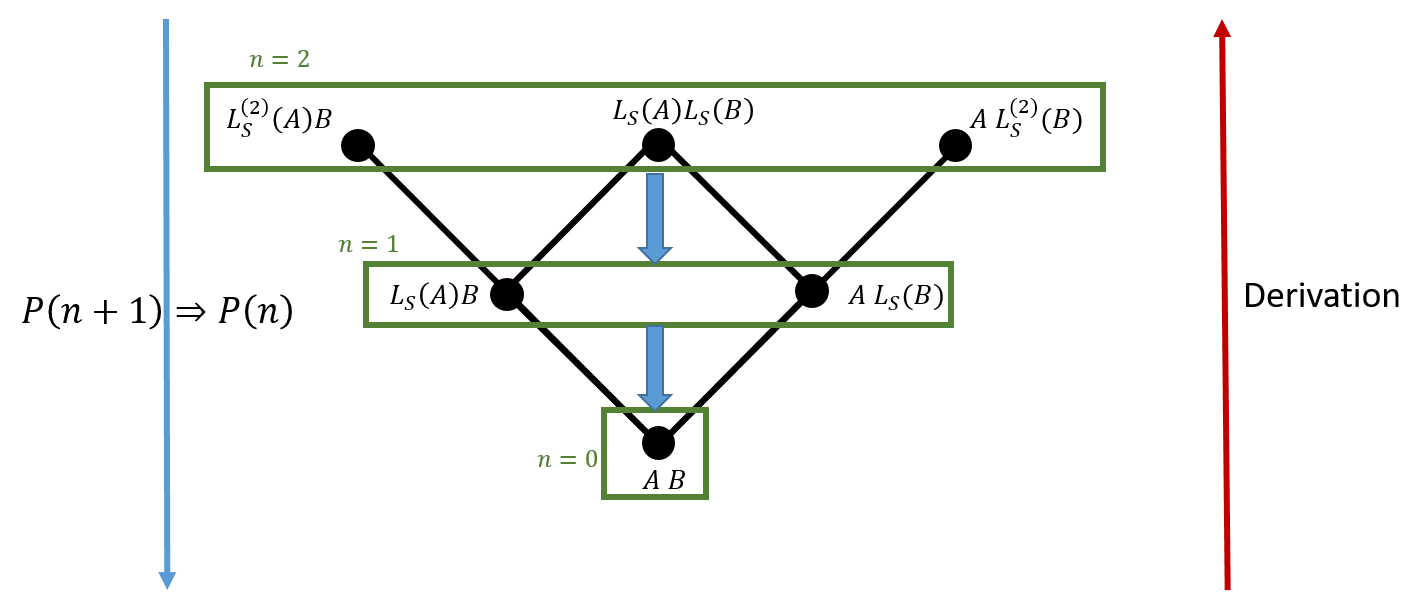
\includegraphics[width=0.9\linewidth]{Pics/image-pascal.png}
      \caption{Inverse Pascal triangle structure that appears under the regularity condition for the pair of operators $(A, B)$. Deriving corresponds to creating two upwards branches to the left (derive $A$) and to the right (derive $B$). The implication $\mathcal{P}(n+1) \implies \mathcal{P}(n)$ goes downwards.}
      \label{fig:image-pascal}
    \end{figure}
\end{center}
    
\chapter{Derivation of Quantum Langevin Equation} \label{2-langevin}
    In this appendix, we present two derivations of the quantum Langevin equation. The first is more general and allows to add many photon loss. The second is based on a more physical model which incorporates two-photon loss.

\section{General Derivation}
This derivation is inspired by the proof of the usual quantum Langevin equation given by Prof. Zaki Leghtas in the class Cavity and Circuit QED in the second semester of the ICFP - Quantum Physics Master 2. The following derivation generalizes the result for any number $\nu$ of photon loss and includes potential jump operators $L_n$ that can affect the cavity from the inside (for eg. dephasing).

\subsubsection{Presentation of the Problem}

We consider a cavity of frequency $\Omega$, whose Unitary evolution is given by $H$ and which is coupled to free propagating modes $b_q$ of frequencies $\omega_q$. The Hamiltonian of the bath is $H_{\text{bath}} = \sum_q \omega_q b^\dagger_q b_q$. Since we consider many photon losses, the modes that matter are the ones such that $\omega_q \approx \nu \Omega$, $\nu \ge 1$. Therefore, we are justified in taking the continuous limit and introducing fictitious modes of negative frequencies. The Hamiltonian can be written in the following manner $H_{\text{bath}} = \int_{-\infty}^\infty d\omega \ \hbar \omega \ b^\dagger_\omega b_\omega$. The modes $b_\omega$ satisfy the commutation relations: $\commutator{b_\omega}{b^\dagger_{\omega'}} = \delta(\omega - \omega')$. $b_\omega$ are propagating modes and have the dimension $T^{\frac{1}{2}}$.

Applying the rotating wave (i.e.\@~only conserving the terms that conserve energy) and the Markov approximations (i.e.\@~the coupling constant has no characteristic frequency), we can write the interaction Hamiltonian

\begin{equation}
    H_{\text{int}} = \sum_{\nu = 1}^\infty \frac{\hbar}{\sqrt{2 \pi}} \int_{-\infty}^\infty d\omega \ \sqrt{\kappa_\nu} \left(a^\nu b^\dagger_\omega + a^{\dagger \nu} b_\omega\right),
\end{equation}
such that the total Hamiltonian is finally given by: $H_{\text{tot}} = H + H_{\text{bath}} + H_{\text{int}}$.

\subsubsection{Heisenberg-Langevin Equations}

We write the Heisenberg-Langevin equations for $a(t)$ and $b_\omega(t)$:

\begin{eqnarray}
    \timeDeriv{a} &=& \ihbar \commutator{a}{H_{\text{tot}}} + \frac{1}{2} \sum_n \left(L^\dagger_n \commutator{a}{L_n} - \commutator{a}{L^\dagger_n} L_n\right) \nonumber\\
    &=& \ihbar \commutator{a}{H} + \frac{1}{2} \sum_n \left(L^\dagger_n \commutator{a}{L_n} - \commutator{a}{L^\dagger_n} L_n\right) \nonumber + \sum_{\nu = 1}^\infty \frac{-i}{\sqrt{2 \pi}} \int_{-\infty}^\infty d\omega \ \sqrt{\kappa_\nu} \nu a^{\dagger (\nu-1)} b_\omega\\
    \timeDeriv{b_\omega} &=& -i \omega b_\omega + \sum_{\nu = 1}^\infty \frac{-i}{\sqrt{2 \pi}} \sqrt{\kappa_\nu} a^\nu
\end{eqnarray}

We take an initial time $t_0$ defined by the input $b_\omega(t_0)$ and solve the second differential equation:

\begin{equation}
    b_\omega(t) = b_\omega(t_0) e^{-i \omega (t - t_0)} - i \sum_{\nu = 1}^\infty \sqrt{\frac{\kappa_\nu}{2 \pi}} \int_{t_0}^t dt' e^{-i \omega (t - t')} a^\nu(t')
\end{equation}

We inject it in the differential equation of $a(t)$:

\begin{eqnarray}
    \timeDeriv{a} &=& \ihbar \commutator{a}{H} + \frac{1}{2} \sum_n \left(L^\dagger_n \commutator{a}{L_n} - \commutator{a}{L^\dagger_n} L_n\right) + \sum_{\nu = 1}^\infty \frac{-i}{\sqrt{2 \pi}} \int_{-\infty}^\infty d\omega \ \sqrt{\kappa_\nu} \nu a^{\dagger (\nu-1)} b_\omega(t_0) e^{-i \omega (t - t_0)} \nonumber\\
    &-& \sum_{\nu = 1}^\infty \frac{\kappa_\nu}{2 \pi} \nu \int_{-\infty}^\infty d\omega \int_{t_0}^t dt' e^{-i \omega (t - t')} a^{\dagger (\nu-1)}(t) a^\nu(t')\nonumber\\
    &=& \ihbar \commutator{a}{H} + \frac{1}{2} \sum_n \left(L^\dagger_n \commutator{a}{L_n} - \commutator{a}{L^\dagger_n} L_n\right) + \sum_{\nu = 1}^\infty \frac{-i}{\sqrt{2 \pi}} \int_{-\infty}^\infty d\omega \ \sqrt{\kappa_\nu} \nu a^{\dagger (\nu-1)} b_\omega(t_0) e^{-i \omega (t - t_0)} \nonumber\\
    &-& \sum_{\nu = 1}^\infty \kappa_\nu\nu  \int_{t_0}^t dt' a^{\dagger (\nu-1)}(t) a^\nu(t') \int_{-\infty}^\infty \frac{d\omega}{2 \pi} \ e^{-i \omega (t - t')}
\end{eqnarray}

To simplify the last term, we use the identities: $\int_{-\infty}^\infty \frac{d\omega}{2 \pi} \ e^{-i \omega (t - t')} = \delta(t - t')$ and $\int_{t_0}^t  dt' \ \delta(t - t') = \int_0^{t-t_0}  d\tau \ \delta(\tau) = \int_0^\infty  d\tau \ \delta(\tau) = \int_0 \frac{1}{2}$. We get:

\begin{eqnarray}
    \timeDeriv{a} &=& \ihbar \commutator{a}{H} + \frac{1}{2} \sum_n \left(L^\dagger_n \commutator{a}{L_n} - \commutator{a}{L^\dagger_n} L_n\right) - \sum_{\nu = 1}^\infty \nu \sqrt{\kappa_\nu} a^{\dagger (\nu-1)} \frac{i}{\sqrt{2 \pi}} \int_{-\infty}^\infty d\omega \ b_\omega(t_0) e^{-i \omega (t - t_0)} \nonumber\\
    &-& \sum_{\nu = 1}^\infty \frac{\nu \kappa_\nu}{2} a^{\dagger (\nu-1)} a^\nu
\end{eqnarray}

We introduce $a_{\text{in}}(t) \equiv \frac{i}{\sqrt{2 \pi}} \int_{-\infty}^\infty d\omega \ b_\omega(t_0) e^{-i \omega (t - t_0)}$ where $a_{\text{in}}(t)$ has the dimension $T^{-\frac{1}{2}}$. We finally get:
\begin{equation}
    \timeDeriv{a} = \ihbar \commutator{a}{H} + \frac{1}{2} \sum_n \left(L^\dagger_n \commutator{a}{L_n} - \commutator{a}{L^\dagger_n} L_n\right) - \sum_{\nu = 1}^\infty \nu a^{\dagger (\nu-1)} \left( \sqrt{\kappa_\nu}  a_{\text{in}}(t) + \frac{\kappa_\nu}{2}a^\nu \right)
\end{equation}

\section{Two-Cavity Model}
We present a more realistic model based on the devices of Alice \& Bob. We will try to find the necessary hypotheses to recover the equation~\autoref{generalized-langevin} we found previously.

\subsection{Model}

Let us consider the model of two cavities corresponding to the annihilators $a$ and $b$ respectively. We consider that the first cavity is the cavity of interest (called the \textit{memory}) whose Unitary evolution is given by the Hamiltonian $H$. The memory is supposed to be lossless. The second cavity is used to induce two photon loss (called the \textit{buffer}). The second cavity corresponds to a free evolving mode $H_b = \hbar \omega b^\dagger b$ with one photon loss given by the rate $\kappa$. Further, we suppose that the second cavity is driven by the input field $b_{\text{in}}(t)$ To obtain two-photon loss, we consider the interaction Hamiltonian $H_{\text{int}} = \hbar g \left(a^{\dagger 2} b + a^2 b^\dagger\right)$. 

\subsection{Heisenberg-Langevin Equations}

We write the standard quantum Langevin equations:

\begin{eqnarray}
    \timeDeriv{a} &=& \ihbar \commutator{a}{H} - 2 i g a^\dagger b\\
    \timeDeriv{b} &=& -i \omega b - i g a^2 -\frac{\kappa}{2} b -\sqrt{\kappa} b_{\text{in}}
\end{eqnarray}

The second equation is an unhomogeneous linear equation and can be solved directly:

\begin{equation}
    b(t) = e^{-\left(i \omega + \frac{\kappa}{2}\right) (t - t_0)} b(t_0) - i g \int_{t_0}^t dt' e^{-\left(i \omega + \frac{\kappa}{2}\right) (t - t')} a^2(t') - \sqrt{\kappa} \int_{t_0}^t dt' e^{-\left(i \omega + \frac{\kappa}{2}\right) (t - t')} b_{\text{in}}(t')
\end{equation}

We take the \textbf{long time limit}: $\kappa (t-t_0) \gg 1$, allowing us to drop the first term:

\begin{equation}
    b(t) \approx - i g \int_{t_0}^t dt' e^{-\left(i \omega + \frac{\kappa}{2}\right) (t - t')} a^2(t') - \sqrt{\kappa} \int_{t_0}^t dt' e^{-\left(i \omega + \frac{\kappa}{2}\right) (t - t')} b_{\text{in}}(t')
\end{equation}

Further, we consider the \textbf{slow evolution approximation} which stipulates that $a(t')$ evolves on time scales much larger than $\frac{1}{\kappa}$. This allows us to write:

\begin{equation}
    \int_{t_0}^t dt' e^{-\left(i \omega + \frac{\kappa}{2}\right) (t - t')} a^2(t') \approx a^2(t) \int_{t_0}^t dt' e^{-\left(i \omega + \frac{\kappa}{2}\right) (t - t')} \approx \frac{2}{\kappa} a^2(t)
\end{equation}

Additionally, we introduce:

\begin{equation}
    a_{\text{in}}(t) \equiv -i \frac{\kappa}{2} \int_{t_0}^t dt' e^{-\left(i \omega + \frac{\kappa}{2}\right) (t - t')} b_{\text{in}}(t')
\end{equation}

We finally get the equation:

\begin{equation}
    \timeDeriv{a} = \ihbar \commutator{a}{H} - \frac{4 g^2}{\kappa} a^\dagger a^2 - 2 \frac{2 g}{\sqrt{\kappa}} a^\dagger a_{\text{in}}(t)
\end{equation}

We thus recover the previous equation. Further, we see that the decay rate is given by the ratio $\eta \equiv \frac{4 g^2}{\kappa}$, which looks like the Purcell effect constant~\cite{purcell1946optical}.
    
\chapter{Expression of Some Quantities as a Function of Moments} \label{app-all-moments}
    The goal of this appendix is to show how to express different quantities that are used to characterize the state. These quantities will not be introduced here for the sake of briefness. A good introduction to quasi-probabilities can be found in~\cite{weiestrass_trans_ref, walls_milburn, explo_quant, wiki-Glauber–Sudarshan, wiki-Husimi, wiki-Wigner}. For the sake of simplicity, we limit ourselves to one-mode states. All the computations of this part are done in the \textbf{Schrödinger picture}. The final result does not depend on the representation.

\section{Quasi-Probabilities}
The goal of this part is to express the $P-$distribution, Wigner function and $Q$ Husimi function as a function of the moments. We limit ourselves to one mode where the quasi-probabilities are usually used. We will prove the following result:
\begin{theorem}[Expression of the Quasi-Probabilities in Function of Moments]
The $P-$distribution can be written as:
\begin{equation} \label{p_distrib_moment}
    P(\beta, \beta^*) =  \sum_{j=0}^\infty \sum_{k=0}^\infty \frac{\average{a^{\dagger j} a^k}}{j! k!} (-1)^{j+k} \frac{\partial^{j+k}}{\partial \beta^{* j} \partial \beta^k}  \delta(\beta, \beta^*)
\end{equation}

The Wigner function can be expressed as:
\begin{equation} \label{eq-wigner-moments}
    W(\alpha, \alpha^*) = \frac{2 e^{-2 |\alpha|^2}}{\pi} \sum_{j=0}^\infty \sum_{k=0}^\infty \frac{\average{a^{\dagger j} a^k}}{j! k!} 2^{k+j} \sum_{r = 0}^{\min(j, k)} \binom{j}{r}  \frac{k!}{(k-r)!} (-1)^r \frac{\alpha^{* (k-r)} \alpha^{j-r}}{2^r}
\end{equation}

Finally, the Husimi function is given by:
\begin{eqnarray} \label{eq-q-moments}
     Q(\alpha, \alpha^*) &=& \frac{e^{-|\alpha|^2}}{\pi} \sum_{j=0}^\infty \sum_{k=0}^\infty \sum_{r = 0}^{\min(j, k)} (-1)^r \frac{\average{a^{\dagger j} a^k}}{j! k!} \binom{j}{r}  \frac{k!}{(k-r)!} \alpha^{* (k-r)} \alpha^{j-r}
\end{eqnarray}
\end{theorem}

\begin{proof}
To prove this theorem, we recall the expression of the $P-$distribution~\cite{khan2021physical}:

\begin{equation}
    P(\beta, \beta^*) = \int \frac{d^2z}{\pi^2} M(z, z^*) e^{-i \beta z}e^{-i \beta^* z^*}
\end{equation}

with $M(z, z^*) = \average{e^{i z^* a^\dagger} e^{i z a}} = \sum_{j=0}^\infty \sum_{k=0}^\infty \frac{\left(i z^*\right)^j \left(i z\right)^k}{j! k!} \average{a^{\dagger j} a^k}$. Thus:

\begin{equation} 
    P(\beta, \beta^*) =  \sum_{j=0}^\infty \sum_{k=0}^\infty \frac{\average{a^{\dagger j} a^k}}{j! k!} \int \frac{d^2z}{\pi^2} \left(i z^*\right)^j \left(i z\right)^k e^{-i \beta z}e^{-i \beta^* z^*}
\end{equation}

We introduce the integral:

\begin{equation}
    I_{j k}(\beta, \beta^*) =  \int \frac{d^2z}{\pi^2} \left(i z^*\right)^j \left(i z\right)^k e^{-i \beta z}e^{-i \beta^* z^*} = (-1)^{j+k} \frac{\partial^{j+k}}{\partial \beta^{* j} \partial \beta^k} \int \frac{d^2z}{\pi^2} e^{-i \beta z}e^{-i \beta^* z^*}
\end{equation}

where: $\int \frac{d^2z}{\pi^2} e^{-i \beta z}e^{-i \beta^* z^*} = \delta(\beta, \beta^*)$. Thus:

\begin{equation}
    P(\beta, \beta^*) =  \sum_{j=0}^\infty \sum_{k=0}^\infty \frac{\average{a^{\dagger j} a^k}}{j! k!} (-1)^{j+k} \frac{\partial^{j+k}}{\partial \beta^{* j} \partial \beta^k}  \delta(\beta, \beta^*)
\end{equation}

Since we know that a state is fully characterized by its $P-$distribution, we conclude that a state is fully characterized by its moments. We can relate the Wigner function to the $P-$distribution using the Weiestrass transform or called Gaussian smoothing~\cite{weiestrass_trans_ref}:

\begin{eqnarray} \label{gaussian_smooth}
    W(\alpha, \alpha^*) &=& 2 \int \frac{d^2 \beta}{\pi} P(\beta, \beta^*) e^{-2 (\beta - \alpha) (\beta^* - \alpha^*)}\\
    &=& 2 \sum_{j=0}^\infty \sum_{k=0}^\infty \frac{\average{a^{\dagger j} a^k}}{j! k!} (-1)^{j+k} \int \frac{d^2 \beta}{\pi} e^{-2 (\beta - \alpha) (\beta^* - \alpha^*)} \frac{\partial^{j+k}}{\partial \beta^{* j} \partial \beta^k}  \delta(\beta, \beta^*) \nonumber\\
    &=& 2 \sum_{j=0}^\infty \sum_{k=0}^\infty \frac{\average{a^{\dagger j} a^k}}{j! k!} \left[\frac{\partial^{j+k}}{\partial \beta^{* j} \partial \beta^k} e^{-2 (\beta - \alpha) (\beta^* - \alpha^*)}\right]_{\beta = 0, \beta^* = 0} \nonumber\\
    &=& \frac{2}{\pi} \sum_{j=0}^\infty \sum_{k=0}^\infty \frac{\average{a^{\dagger j} a^k}}{j! k!} \left[\frac{\partial^{j}}{\partial \beta^{* j}} (-2)^k (\beta^* -\alpha^*)^k e^{-2 (\beta - \alpha) (\beta^* - \alpha^*)}\right]_{\beta = 0, \beta^* = 0} \nonumber
\end{eqnarray}

Using Bernoulli's identity for the derivative of a product, we find:

\begin{eqnarray}    
     W(\alpha, \alpha^*) &=& \frac{2}{\pi} \sum_{j=0}^\infty \sum_{k=0}^\infty \frac{\average{a^{\dagger j} a^k}}{j! k!} (-2)^k\nonumber\\ &\times& \sum_{r = 0}^{\min(j, k)} \binom{j}{r} \left[\frac{\partial^{r}}{\partial \beta^{* r}} (\beta^* - \alpha^*)^k \right]_{\beta = \beta^* = 0} \left[ \frac{\partial^{j-r}}{\partial \beta^{* (j-r)}}e^{-2 (\beta - \alpha) (\beta^* - \alpha^*)}\right]_{\beta =\beta^* = 0} \nonumber\\
     &=& \frac{2}{\pi} \sum_{j=0}^\infty \sum_{k=0}^\infty \frac{\average{a^{\dagger j} a^k}}{j! k!} (-2)^k \nonumber\\
     &\times& \sum_{r = 0}^{\min(j, k)} \binom{j}{r}  \left[\frac{k!}{(k-r)!}  (\beta^* - \alpha^*)^{k-r} \right]_{\beta = \beta^* = 0} \left[(-2)^{j-r} (\beta - \alpha)^{j-r}  e^{-2 (\beta - \alpha) (\beta^* - \alpha^*)}\right]_{\beta =\beta^* = 0}\nonumber\\
     &=& \frac{2}{\pi} \sum_{j=0}^\infty \sum_{k=0}^\infty \frac{\average{a^{\dagger j} a^k}}{j! k!} (-2)^k \sum_{r = 0}^{\min(j, k)} \binom{j}{r}  \frac{k!}{(k-r)!} (-\alpha^*)^{k-r} (-2)^{j-r} (-\alpha)^{j-r} e^{-2 |\alpha|^2}\nonumber\\
     &=& \frac{2 e^{-2 |\alpha|^2}}{\pi} \sum_{j=0}^\infty \sum_{k=0}^\infty \frac{\average{a^{\dagger j} a^k}}{j! k!} 2^{k+j} \sum_{r = 0}^{\min(j, k)} \binom{j}{r}  \frac{k!}{(k-r)!} (-1)^r \frac{\alpha^{* (k-r)} \alpha^{j-r}}{2^r}
\end{eqnarray}

We finally find:
\begin{equation}
    W(\alpha, \alpha^*) = \frac{2 e^{-2 |\alpha|^2}}{\pi} \sum_{j=0}^\infty \sum_{k=0}^\infty \frac{\average{a^{\dagger j} a^k}}{j! k!} 2^{k+j} \sum_{r = 0}^{\min(j, k)} \binom{j}{r}  \frac{k!}{(k-r)!} (-1)^r \frac{\alpha^{* (k-r)} \alpha^{j-r}}{2^r}
\end{equation}

Similarly, the Husimi $Q-$distribution is related to the $P-$distribution by the Gaussian smoothing~\cite{weiestrass_trans_ref}:
\begin{eqnarray}
    Q(\alpha, \alpha^*) &=& \int \frac{d^2 \beta}{\pi} P(\beta, \beta^*) e^{-|\alpha - \beta|^2}\\
    &=& \sum_{j=0}^\infty \sum_{k=0}^\infty \frac{\average{a^{\dagger j} a^k}}{j! k!} (-1)^{j+k} \int \frac{d^2 \beta}{\pi} e^{-(\beta - \alpha) (\beta^* - \alpha^*)} \frac{\partial^{j+k}}{\partial \beta^{* j} \partial \beta^k}  \delta(\beta, \beta^*) \nonumber\\
    &=& \frac{1}{\pi} \sum_{j=0}^\infty \sum_{k=0}^\infty \frac{\average{a^{\dagger j} a^k}}{j! k!} (-1)^{j+k} \left[\frac{\partial^{j+k}}{\partial \beta^{* j} \partial \beta^k} e^{(\beta - \alpha) (\beta^* - \alpha^*)}\right]_{\beta = 0, \beta^* = 0} \nonumber\\
    &=& \frac{1}{\pi} \sum_{j=0}^\infty \sum_{k=0}^\infty \frac{\average{a^{\dagger j} a^k}}{j! k!} \left[\frac{\partial^{j}}{\partial \beta^{* j}} (-1)^k (\beta^* -\alpha^*)^k e^{-(\beta - \alpha) (\beta^* - \alpha^*)}\right]_{\beta = 0, \beta^* = 0} \nonumber\\
\end{eqnarray}

Using Bernoulli's identity for the derivative of a product and evaluating at $(0, 0)$, we find:

\begin{eqnarray}
     Q(\alpha, \alpha^*) &=& \frac{e^{-|\alpha|^2}}{\pi} \sum_{j=0}^\infty \sum_{k=0}^\infty \sum_{r = 0}^{\min(j, k)} (-1)^r \frac{\average{a^{\dagger j} a^k}}{j! k!} \binom{j}{r}  \frac{k!}{(k-r)!} \alpha^{* (k-r)} \alpha^{j-r}
\end{eqnarray}
\end{proof}
\subsection{Sanity Check: Coherent State}
In this part, we verify the relations \autoref{p_distrib_moment} and \autoref{eq-wigner-moments} for a one-mode coherent state $\ket{\gamma}$.

\subsubsection{$P-$distribution}
For the state $\ket{\gamma}$, we know that the $P-$distribution is given by $P(\beta, \beta^*) =  \delta(\beta - \gamma, \beta^* - \gamma^*)$. Further, let $\phi(\beta, \beta^*)$ be a function that admits a Taylor power series expansion (recall that the $P-$distribution  is a distribution, not a function). We have:

\begin{eqnarray}
    \int d^2 \beta \ P(\beta, \beta^*) \phi(\beta, \beta^*) &=&  \phi(\gamma, \gamma^*) \nonumber\\
    &=&  \sum_{j=0}^\infty \sum_{k=0}^\infty \frac{\gamma^{* j} \gamma^k}{j! k!} \frac{\partial^{j+k} \phi}{\partial \beta^{* j} \partial \beta^k}(0, 0) \nonumber\\
    &=&  \sum_{j=0}^\infty \sum_{k=0}^\infty \frac{\gamma^{* j} \gamma^k}{j! k!} (-1)^{j+k} \int d^2 \beta \ \phi(\beta, \beta^*) \frac{\partial^{j+k} \delta}{\partial \beta^{* j} \partial \beta^k}(\beta, \beta^*)
\end{eqnarray}

Since this equality is true for any $\phi(\beta, \beta^*)$, we deduce that:

\begin{equation}
    P(\beta, \beta^*) = \sum_{j=0}^\infty \sum_{k=0}^\infty \frac{\gamma^{* j} \gamma^k}{j! k!} (-1)^{j+k} \frac{\partial^{j+k}}{\partial \beta^{* j} \partial \beta^k} \delta(\beta, \beta^*)
\end{equation}

which is~\autoref{p_distrib_moment} for the coherent state $\ket{\gamma}$.

\subsubsection{Wigner Function and Husimi Function}
For the state $\ket{\gamma}$, we know that the Wigner function is given by $W(\alpha, \alpha^*) =  \frac{2}{\pi} e^{-2 (\gamma - \alpha) (\gamma^* - \alpha^*)}$ (this can be seen from~\autoref{gaussian_smooth}). $W(\alpha, \alpha^*)$ can be given by the Taylor expansion:

\begin{equation}
    W(\alpha, \alpha^*) = \frac{2}{\pi} \sum_{j=0}^\infty \sum_{k=0}^\infty \frac{\gamma^{* j} \gamma^k}{j! k!} \left[\frac{\partial^{j+k}}{\partial \gamma^{* j} \partial \gamma^k} e^{-2 (\gamma - \alpha) (\gamma^* - \alpha^*)}\right]_{\gamma = \gamma^* = 0}
\end{equation}

Expanding the derivatives and evaluating them at $(0,0)$ corresponds to~\autoref{eq-wigner-moments} for the state $\ket{\gamma}$. We obtain a similar result for~\autoref{eq-q-moments} with $Q(\alpha, \alpha^*) =  \frac{1}{\pi} e^{-(\gamma - \alpha) (\gamma^* - \alpha^*)}$

\section{Probability of Number Occupation}

In this part, we evaluate $\pr{n}$, the probability of being occupied by $n$ photons. The goal is to prove the following result:
\begin{theorem}[Expression of the Probability of Occupation in Function of Moments]
    $\pr{n}$ is given by:
    \begin{equation} \label{eq_pr_n_moments}
    \pr{n} = \frac{1}{n!} \sum_{k=0}^\infty (-1)^k \frac{\average{a^{\dagger (k+n)} a^{k+n}}}{k!}
    \end{equation}
\end{theorem}

\begin{proof}
We introduce the $P-$distribution:

\begin{equation}
    \pr{n} = \mel{n}{\rho}{n} = \int d^2 \alpha P(\alpha, \alpha^*) \braket{n}{\alpha} \braket{\alpha}{n} = \int d^2 \alpha P(\alpha, \alpha^*) \frac{|\alpha|^{2 n}}{n!} e^{-|\alpha|^2} = \int d^2 \alpha P(\alpha, \alpha^*) \frac{\alpha^{* n} \alpha^{n}}{n!} e^{-\alpha^* \alpha}
\end{equation}

Using~\autoref{p_distrib_moment}, we have:
\begin{eqnarray}
    \pr{n} &=& \sum_{j=0}^\infty \sum_{k=0}^\infty \frac{\average{a^{\dagger j} a^k}}{j! k!} (-1)^{j+k} \int d^2 \alpha \frac{\alpha^{* n} \alpha^{n}}{n!} e^{-\alpha^* \alpha} \frac{\partial^{j+k}}{\partial \alpha^{* j} \partial \alpha^k}  \delta(\alpha, \alpha^*)\nonumber\\
    &=& \sum_{j=0}^\infty \sum_{k=0}^\infty \frac{\average{a^{\dagger j} a^k}}{j! k! n!} \left[\frac{\partial^{j+k}}{\partial \alpha^{* j} \partial \alpha^k} \alpha^{* n} \alpha^{n} e^{-\alpha^* \alpha} \right]_{\alpha = \alpha^* = 0}\nonumber
\end{eqnarray}

Using Bernoulli's identity twice, we get:

\begin{eqnarray}
    \frac{\partial^{j+k}}{\partial \alpha^{* j} \partial \alpha^k} \alpha^{* n} \alpha^{n} e^{-\alpha^* \alpha} &=& \frac{\partial^j}{\partial \alpha^{* j}} \left\{\alpha^{* n} \sum_{r = 0}^{k} \binom{k}{r} \left(\frac{\partial^r}{\partial \alpha^{r}} \alpha^{n}\right) \left(\frac{\partial^{k-r}}{\partial \alpha^{k-r}} e^{-\alpha^* \alpha}\right) \right\}\nonumber\\
    &=& \frac{\partial^j}{\partial \alpha^{* j}} \left\{\alpha^{* n} \sum_{r = 0}^{\min(k,n)} \binom{k}{r} \frac{n!}{(n-r)!} \alpha^{n-r} (-\alpha^*)^{k-r} e^{-\alpha^* \alpha}\right\}\nonumber\\
    &=& \sum_{r = 0}^{\min(k,n)} \binom{k}{r} \frac{n!}{(n-r)!} (-1)^{k-r} \alpha^{n-r} \frac{\partial^j}{\partial \alpha^{* j}}\left(\alpha^{* (n+k-r)} e^{-\alpha^* \alpha}\right)\nonumber\\
    &=& \sum_{r = 0}^{\min(k,n)} \binom{k}{r} \frac{n!}{(n-r)!} (-1)^{k-r} \alpha^{n-r} \sum_{s = 0}^{j} \binom{j}{s} \left(\frac{\partial^s}{\partial \alpha^{s}} \alpha^{n+k-r}\right) \left(\frac{\partial^{j-s}}{\partial \alpha^{j-s}} e^{-\alpha^* \alpha}\right)\nonumber\\
    &=& \sum_{r = 0}^{\min(k,n)} \sum_{s = 0}^{\min(j,n+k-r)} \binom{k}{r} \binom{j}{s} \frac{n! (n+k-r)!}{(n-r)! (n+k-r-s)!} \nonumber\\ &\times& (-1)^{k+j-r-s} \alpha^{n+j-r-s} \alpha^{* (n+k-r-s)} e^{-\alpha^* \alpha}
\end{eqnarray}

Evaluating at $\alpha = 0$, finding the nonzero term corresponds to solving the system:

\begin{eqnarray} \label{eq_sys_1}
    n + j &=& r + s\\ \label{eq_sys_2}
    n + k &=& r + s\\ \label{eq_sys_3}
    0 \le s &\le& \min(j,n+k-r)\\ \label{eq_sys_4}
    0 \le r &\le& \min(k,n)
\end{eqnarray}

\autoref{eq_sys_1} and~\autoref{eq_sys_2} imply that $j = k$. Further, \autoref{eq_sys_4} implies that $r \le n$, \autoref{eq_sys_3} becomes $0 \le s \le k$. Therefore, satisfying~\autoref{eq_sys_2} imposes that $s = k$ and $r = n$, which implies that $n \le k$. Thus, we have the simple expression:

\begin{equation}
    \pr{n} = \frac{1}{n!} \sum_{k=0}^\infty (-1)^k \frac{\average{a^{\dagger (k+n)} a^{k+n}}}{k!}
\end{equation}
\end{proof}
\begin{corollary}
    $\pr{n}$ depends only on the averages $\average{a^{\dagger q} a^{q}}$ for $q \ge n$.
\end{corollary}

\subsection{Sanity Checks}

We test the validity of the formula~\autoref{eq_pr_n_moments} by taking the case of a coherent state and a Fock state.

\subsubsection{Coherent State $\ket{\alpha}$}

We know that: $\average{a^{\dagger (k+n)} a^{k+n}} = |\alpha|^{2 (k+n)}$, thus:

\begin{equation}
    \frac{1}{n!} \sum_{k=0}^\infty (-1)^k \frac{\average{a^{\dagger (k+n)} a^{k+n}}}{k!} = \frac{1}{n!} \sum_{k=0}^\infty (-1)^k \frac{|\alpha|^{2 (k+n)}}{k!} = \frac{|\alpha|^{2 n}}{n!} \sum_{k=0}^\infty (-1)^k \frac{|\alpha|^{2 k}}{k!} = \frac{|\alpha|^{2 n}}{n!} e^{-|\alpha|^2}
\end{equation}

which is the correct value

\subsubsection{Fock State $\ket{\nu}$}

We have $\mel{\nu}{a^{\dagger (k+n)} a^{k+n}}{\nu} = \left\Vert a^{k+n} \ket{\nu} \right\Vert^2$, thus:

\begin{eqnarray}
    \mel{\nu}{a^{\dagger (k+n)} a^{k+n}}{\nu} &=& \frac{\nu!}{(\nu-k-n)!} \ , \ k \le \nu - n\\
    \mel{\nu}{a^{\dagger (k+n)} a^{k+n}}{\nu} &=& 0 \ , \ k > \nu - n
\end{eqnarray}

Thus, if $n > \nu$, $\frac{1}{n!} \sum_{k=0}^\infty (-1)^k \frac{\average{a^{\dagger (k+n)} a^{k+n}}}{k!} = 0$. Otherwise:
\begin{equation}
    \frac{1}{n!} \sum_{k=0}^\infty (-1)^k \frac{\average{a^{\dagger (k+n)} a^{k+n}}}{k!} = \sum_{k=0}^{\nu - n} (-1)^k \frac{\nu!}{(\nu-k-n)!} = \frac{\nu!}{(\nu-n)!} \sum_{k=0}^{\nu - n} (-1)^k \frac{(\nu-n)!}{(\nu-k-n)!} = \frac{\nu!}{(\nu-n)!} (1-1)^{\nu - n}
\end{equation}

Therefore: $\frac{1}{n!} \sum_{k=0}^\infty (-1)^k \frac{\average{a^{\dagger (k+n)} a^{k+n}}}{k!} = \delta_{\nu, n}$, which is the exact value.
    
\chapter{Analytical Expressions for Some Hamiltonians} \label{app-analytic-exp}
    In this part, we solve exactly some Hamiltonians and give examples where our methods for analytical resolution fail. The analytical expressions given here were not found in the literature.

\section{Results and Techniques}
In this section, we present the time-ordered exponential and show how we can use it for solving some differential systems.

\subsection{Time-Ordered Exponential}
\subsubsection{Definition}
The time-ordered exponential is defined as the solution of the initial value problem \cite{wiki_time_exp, course-time_exp}:

\begin{eqnarray}
    \timeDeriv{\texp{A}} &=& A(t) \texp{A}\\
    \texp{A}(t = 0) &=& \mathbb{1}
\end{eqnarray}

$\texp{A}$ can be expressed as the following series~\cite{course-time_exp}:

\begin{equation}
    \texp{A} = \mathbb{1} + \sum_{n=1}^\infty \int_{0}^{t} dt_1 \int_{0}^{t_1} dt_2 ... \int_{0}^{t_{n-1}} dt_n \ A(t_1) ... A(t_n)
\end{equation}

It turns out the time ordered exponential is different from the usual exponential when the operators $\{A(t')\}_{t'}$ do not commute. Indeed, time ordering refers to putting the operators in an increasing value of time from the right to the left. This ensures that they are applied in a chronological order.

\subsubsection{Technique}

Let us consider the evolution of the operator $O(t)$. The following theorem gives the expression of $O(t)$ in a particular case:

\begin{theorem}[Resolution with Time-Ordered Exponential] \label{th_res-toe}
    Supposes that: $\timeDeriv{O} = \mathbb{F}(t) O$, then:
    \begin{equation}
        O(t) = \texp{\mathbb{F}} O(0)
    \end{equation}
\end{theorem}

\begin{proof}
    We have: $\texp{\mathbb{F}}(t=0) O(0) = O(0)$ and 
    $$\timeDeriv{\texp{\mathbb{F}} O(0)} = \mathbb{F}(t) \texp{\mathbb{F}} O(0).$$ Since $O(t)$ and $\texp{\mathbb{F}} O(0)$ satisfy the same differential equation with the same initial condition, we deduce that they are equal.
\end{proof}

Thus, \textit{if} we know how to express $\mathbb{F}(t)$, we fully know the evolution of $O(t)$. In~\autoref{self-kerr-exact-sol}, \autoref{cross-kerr-exact-sol} and~\autoref{gene-exact-sol}, we present examples where this is the case.

\subsection{Derivation with Respect to Operators} \label{int-op}

Many techniques for solving differential equations where the unknown function takes complex values use the identification of an expression as the derivative relative to the complex function. A usual example is the method of separation of variables. Generalizing this approach requires defining derivatives with respect to operators. This is challenging since two operators do not commute in general. This is particularly important when we want to integrate with respect to an operator, which imposes putting the differential on the right or on the left. Nevertheless, this can be done properly \cite{Suzuki1997-zw}. This required introducing commutators. We invite the interested reader to look into the paper \cite{Suzuki1997-zw} where derivatives of powers, exponentials and logarithms, amongst others, are derived. Here, we limit ourselves to an example to illustrate the need for commutators.

Let us consider the differential equation on the operator $X$: $\timeDeriv{X} = \frac{1}{X}$ (in this example, we do not bother whether the equation is well-defined). We might attempt to use the separation of variables and write: $X dX = dt$. Formally, the expression is correct. The next step is to integrate the two expressions from $0$ to $t$. However, this required from us to know the primitive of $X \mapsto X$. Sadly, it is not $X \mapsto \frac{X^2}{2}$. Indeed:

\begin{eqnarray}
    \lim_{h \rightarrow 0} \frac{(X + h dX)^2 - X^2}{h} &=& \lim_{h \rightarrow 0} \frac{X^2 + h X dX + h dX X + h^2 dX^2 - X^2}{h} = X dX + dX X \nonumber\\
    &=& 2 X dX + \commutator{dX}{X} = (2 X + \commutator{.}{X}) dX
\end{eqnarray}

Thus, it is not straightforward to find the primitive of $X \mapsto X$. The method of separation of variables cannot be used directly on operators.

\section{Examples}
In this section, we present some examples where an analytical expression is found and others where we did not manage to do so. We present an explanation for the failure.

\subsection{One-Mode Kerr Hamiltonian} \label{self-kerr-exact-sol}
The self-Kerr Hamiltonian is given by $H = \hbar g a^{\dagger 2} a^2$.

The annihilator $a$ satisfies the differential equation:
\begin{equation}
    \timeDeriv{a} = -2ig a^\dagger a^2 = \left(-2ig a^\dagger a\right) a
\end{equation}

We have:

\begin{equation}
    \timeDeriv{a^\dagger a} = \timeDeriv{a^\dagger} a(t) + a^\dagger(t) \timeDeriv{a} = 0
\end{equation}

Thus, $a^\dagger(t) a(t) = a^\dagger(0) a(0)$. The differential equation is in the form of~\autoref{th_res-toe} and thus:

\begin{equation}
    a(t) = \Texp{-2 i g t a^\dagger(0) a(0)} a(0) = e^{-2 i g t a^\dagger(0) a(0)} a(0)
\end{equation}

\subsubsection{Expression of the moments}
We can use the expression $a(t) = e^{-2 i g t a^\dagger(0) a(0)} a(0)$ to find the time evolution of the moments $\mel{\alpha}{a^{\dagger j}(t) a^k(t)}{\alpha}$ for example.

To do this, we write $a(t) \ket{\alpha}$:
\begin{equation}
    a(t) \ket{\alpha} = e^{-2 i g t a^\dagger(0) a(0)} a(0) \ket{\alpha} = \alpha e^{-2 i g t a^\dagger(0) a(0)} \ket{\alpha} = \alpha e^{-\frac{|\alpha|^2}{2}} \sum_{n=0}^\infty \frac{\alpha^n}{\sqrt{n!}} e^{-2 i g t n} \ket{n} = \alpha \ket{\alpha e^{-2 i g t}}
\end{equation}
with: $\ket{\beta(t)} \equiv e^{-\frac{|\beta(t)|^2}{2}} \sum_{n=0}^\infty \frac{\beta(t)^n}{\sqrt{n!}} \ket{n}$. Thus, by induction, we have: $a^k(t) \ket{\alpha} = \left(\prod_{l=0}^{k-1} \alpha e^{-2 i l g t} \right) \ket{\alpha e^{-2 i k g t}} = \alpha^k e^{-2 i g t k(k-1)} \ket{\alpha e^{-2 i k g t}}$. Therefore, $\mel{\alpha}{a^{\dagger j}(t) a^k(t)}{\alpha} = \alpha^{* j} \alpha^k e^{-2 i g t [k(k-1) - j(j-1)]} \braket{\alpha e^{-2 i j g t}}{\alpha e^{-2 i k g t}}$, with:

\begin{equation*}
    \braket{\alpha e^{-2 i j g t}}{\alpha e^{-2 i k g t}} = e^{-|\alpha|^2} \sum_{n=0}^\infty \frac{|\alpha|^{2 n} e^{- 2 i (k-j) n g t}}{n!} = e^{-|\alpha|^2} e^{|\alpha|^2 e^{- 2 i (k-j) g t}}.
\end{equation*}

Thus:

\begin{equation}
    \mel{\alpha}{a^{\dagger j}(t) a^k(t)}{\alpha} = \alpha^{* j} \alpha^k e^{-|\alpha|^2} e^{|\alpha|^2 e^{- 2 i (k-j) g t}} \exp{- 2 i g (k - j) (k + j - 1) t}
\end{equation}

\subsection{Cross-Kerr Hamiltonian} \label{cross-kerr-exact-sol}
Let us consider two bosonic modes represented by their annihilators $a$ and $b$. The cross-Kerr Hamiltonian is given by $H = \hbar g a^\dagger b^\dagger b a$. $a(t)$ and $b(t)$ satisfy the equations of evolution:
\begin{eqnarray}
    \timeDeriv{a} &=& -i g b^\dagger b a\\
    \timeDeriv{b} &=& -i g a^\dagger a b
\end{eqnarray}

We have:
\begin{eqnarray}
    \timeDeriv{a^\dagger a} &=& 0\\
    \timeDeriv{b^\dagger b} &=& 0
\end{eqnarray}

Again, the differential system is in the form~\autoref{th_res-toe}, thus:

\begin{eqnarray}
    a(t) &=& \exp{-i g t b^\dagger(0) b(0)} a(0)\\
    b(t) &=& \exp{-i g t a^\dagger(0) a(0)} b(0)
\end{eqnarray}

\subsection{Partial Generalization} \label{gene-exact-sol}
The examples above can be solved without any greater effort if \textit{diagonal quadratic} terms are added to the Hamiltonian. This observation is more general in fact. The same method used in~\autoref{self-kerr-exact-sol} and~\autoref{cross-kerr-exact-sol} can be used for any Hamiltonian in the form: $H = H\left(a^\dagger_1 a_1, ..., a^\dagger_N a_N\right)$ (i.e.\@~each term has the same number of creators and annihilators for each mode). Indeed, in this case, the equation of evolution of the annihilators is of the form of~\autoref{th_res-toe} and $\mathbb{F} = \mathbb{F}\left(a^\dagger_1 a_1, ..., a^\dagger_N a_N\right)$.

Let us show this more rigorously:
\begin{proof}
    $H = H\left(a^\dagger_1 a_1, ..., a^\dagger_N a_N\right)$, thus we can write for the mode $i$, by writing $H$ in normal order for the mode $i$ for example:
    \begin{equation}
        H = \sum_{q=0}^\infty h^{(i)}_q\left(\{a^\dagger_j a_j\}_{j \neq i}\right) a_i^{\dagger q} a_i^q
    \end{equation}
    Therefore, the equation of evolution of $a_i$ is:
    \begin{equation}
        \timeDeriv{a_i} = \ihbar \sum_{q=0}^\infty h^{(i)}_q\left(\{a^\dagger_j a_j\}_{j \neq i}\right) q a_i^{\dagger (q-1)} a_i^q = \left[\ihbar \sum_{q=0}^\infty h^{(i)}_q\left(\{a^\dagger_j a_j\}_{j \neq i}\right) q a_i^{\dagger (q-1)} a_i^{q-1}\right] a_i
    \end{equation}

    Further, using that $\mathbb{F}^\dagger = \mathbb{F}$, we have $\timeDeriv{a^\dagger_j a_j} = 0$, thus 
    this equation is of the form of~\autoref{th_res-toe}, its corresponding $\mathbb{F} = \mathbb{F}\left(a^\dagger_1 a_1, ..., a^\dagger_N a_N\right)$, implying that $\mathbb{F}^\dagger = \mathbb{F}$.
\end{proof}

\chapter{Summary of the Methods} \label{summ-all-meths}
    In this appendix, we present a brief summary of a variety of aspects of the different methods. In \autoref{tab:summ-table}, we present a summary of the different methods that were explored in this report. In \autoref{tab:summ-table-stab}, we present the summary of the stability of the methods. In \autoref{tab:fig-table-stab}, we present many stability plots for the mean field methods.

\begin{landscape}
\begin{center}
    \begin{table}[h!]
    \centering
    \begin{tabular}{|p{3.5cm}|p{4cm}|p{4cm}|p{4cm}|p{4cm}|p{4cm}|}
        \hline
        \textbf{Method} & \texttt{dynamiqs}~\cite{dynamiqs} & \textbf{Usual MF} & \texttt{Truncated Cumulants} & \textbf{TEA} & \textbf{Analytical Expression} \\
        \hline
        \textbf{Followed Quantity} & Density matrix & Moments & Cumulants & Operator $a_i(t)$ in symbolic representation & Exact analytical expression \\
        \hline
        \textbf{Cut-off} & Number of photons (cut-off in the Fock basis) & Degree of the moment, impose some closure relation linking moments of higher degree to moments of lower degrees & Degree of the cumulant, set cumulants to zero beyond some $p$ & Compute the infinite series of operators up to some $p$ & - \\
        \hline
        \textbf{Generality / Validity} & Very general if small number of modes / photons & Limited by how well MF describes the state & Initial sum over Gaussian states & In theory for closed systems, works for open systems in some cases & Requires being able to find the solution \\
        \hline
        \textbf{Advantages} & Can be optimised using linear algebra tools & Fast, accurate for short times. Can be improved with no relative cost using Padé approximate. & Very accurate at short times. More stable than usual MF methods & Can solve for any initial condition. Can compute symbolically for a set of parameters (can be useful for machine learning). & Computing exact analytical expressions numerically is much better than estimating the value numerically (in terms of accuracy, stability, time\ldots)\\
        \hline
        \textbf{Problems / Open Questions} & Many modes with a significant number of photons (for eg.\@~$4$ modes with a cut-off of $\sim 20$ photons per mode) & If non-Gaussian interaction, instability. How to describe non-Gaussian states in general? & Slow, needs to pre-compute equations if machine learning applications. If non-Gaussian interaction, instability. How to describe non-Gaussian states in general? & Small improvement at large time expense. Gives correlations instead of moments. How to deal with open systems properly? & Integrals and differential of operators are tricky. $(A B)_H \neq A_H B_H$ for open systems. Green's function for non-linear systems?\\
        \hline
    \end{tabular}
    \caption{Summary of the methods}
    \label{tab:summ-table}
\end{table}
\end{center}
\end{landscape}

\begin{landscape}
\begin{center}
    \begin{table}[h!]
    \centering
    \begin{tabular}{|p{3.5cm}|p{4cm}|p{4cm}|p{4cm}|p{4cm}|p{4cm}|}
        \hline
        \textbf{Method} & \texttt{dynamiqs}~\cite{dynamiqs} & \textbf{Usual MF} & \texttt{Truncated Cumulants} & \textbf{TEA} & \textbf{Analytical Expression} \\
        \hline
        \textbf{General description} & Very stable if cut-off large enough & Becomes unstable once non-linearity kicks in & Becomes unstable once non-linearity kicks in & Can be made stable using Padé approximate (with no relative cost) & - \\
        \hline
        \textbf{One Photon-Loss} & - & Stabilized & Stabilized & - & - \\
        \hline
        \textbf{Two Photon-Loss} & - & Destabilized & Stabilized & - & - \\
        \hline
        \textbf{Dephasing} & - & Neutral & Neutral & - & - \\
        \hline
        \textbf{$H=a^{\dagger 2} + a^2$ and $L = \sqrt{\kappa} a^2$} & - & Very unstable & Stable \textbf{if} $\alpha$ and $\kappa$ and large enough & - & - \\
        \hline
        
    \end{tabular}
    \caption{Stability of the Methods - Verbal description}
    \label{tab:summ-table-stab}
\end{table}
\end{center}

In general, having higher $p$ is better if stable.
\end{landscape}

\begin{landscape}
\begin{longtable}{|p{3cm}|p{7.2cm}|p{7.2cm}|p{7.2cm}|}
    \hline
    \textbf{Method} & \texttt{Truncated Cumulants} & \texttt{Divide in half}  & \texttt{Minimum cut} \\
    \hline
    \endfirsthead
        
    \textbf{Method} & \texttt{Truncated Cumulants} & \texttt{Divide in half}  & \texttt{Minimum cut} \\
    \hline
    \endhead
        
    \hline
    \endfoot

    \hline
    \endlastfoot
        
    $H=0$ \& $L = \sqrt{\kappa} a$ ; $p=1$ &
    \begin{minipage}{7cm}
        \centering
        \includegraphics[width=\textwidth]{Pics/Stab_1_trunc_cumul.pdf}
    \end{minipage}&
    \begin{minipage}{7cm}
        \centering
        \includegraphics[width=\textwidth]{Pics/Stab_1_divide_in_half.pdf}
    \end{minipage}&
    \begin{minipage}{7cm}
        \centering
        \includegraphics[width=\textwidth]{Pics/Stab_1_min_cut.pdf}
    \end{minipage}\\
    \hline
    $H=0$ \& $L = \sqrt{\kappa} a$ ; $p=2$ &
    \begin{minipage}{7cm}
        \centering
        \includegraphics[width=\textwidth]{Pics/Stab_1_trunc_cumul_p=2.pdf}
    \end{minipage}&
    \begin{minipage}{7cm}
        \centering
        \includegraphics[width=\textwidth]{Pics/Stab_1_divide_in_half_p=2.pdf}
    \end{minipage}&
    \begin{minipage}{7cm}
        \centering
        \includegraphics[width=\textwidth]{Pics/Stab_1_min_cut_p=2.pdf}
    \end{minipage}\\
    \hline
    \hline
    $H=0$ \& $L = \sqrt{\kappa} a^2$ ; $p=2$ &
    \begin{minipage}{7cm}
        \centering
        \includegraphics[width=\textwidth]{Pics/Stab_2_trunc_cumul.pdf}
    \end{minipage}&
    \begin{minipage}{7cm}
        \centering
        \includegraphics[width=\textwidth]{Pics/Stab_2_divide_in_half.pdf}
    \end{minipage}&
    \begin{minipage}{7cm}
        \centering
        \includegraphics[width=\textwidth]{Pics/Stab_2_min_cut.pdf}
    \end{minipage}\\
    \hline
    $H=0$ \& $L = \sqrt{\kappa} a^2$ ; $p=3$ &
    \begin{minipage}{7cm}
        \centering
        \includegraphics[width=\textwidth]{Pics/Stab_2_trunc_cumul_p=3.pdf}
    \end{minipage}&
    \begin{minipage}{7cm}
        \centering
        \includegraphics[width=\textwidth]{Pics/Stab_2_divide_in_half_p=3.pdf}
    \end{minipage}&
    \begin{minipage}{7cm}
        \centering
        \includegraphics[width=\textwidth]{Pics/Stab_2_min_cut_p=3.pdf}
    \end{minipage}\\
    \hline
    $H=0$ \& $L = \sqrt{\kappa} a^2$ ; $p=4$ &
    \begin{minipage}{7cm}
        \centering
        \includegraphics[width=\textwidth]{Pics/Stab_2_trunc_cumul_p=4.pdf}
    \end{minipage}&
    \begin{minipage}{7cm}
        \centering
        \includegraphics[width=\textwidth]{Pics/Stab_2_divide_in_half_p=4.pdf}
    \end{minipage}&
    \begin{minipage}{7cm}
        \centering
        \includegraphics[width=\textwidth]{Pics/Stab_2_min_cut_p=4.pdf}
    \end{minipage}\\
    \hline
    $H=0$ \& $L = \sqrt{\kappa} a^2$ ; $p=5$ &
    \begin{minipage}{7cm}
        \centering
        \includegraphics[width=\textwidth]{Pics/Stab_2_trunc_cumul_p=5.pdf}
    \end{minipage}&
    \begin{minipage}{7cm}
        \centering
        \includegraphics[width=\textwidth]{Pics/Stab_2_divide_in_half_p=5.pdf}
    \end{minipage}&
    \begin{minipage}{7cm}
        \centering
        \includegraphics[width=\textwidth]{Pics/Stab_2_min_cut_p=5.pdf}
    \end{minipage}\\
    \hline
    \hline
    $H=a^2+a^{\dagger 2}$ \& $L = \sqrt{\kappa} a^2$ ; $p=2$ &
    \begin{minipage}{7cm}
        \centering
        \includegraphics[width=\textwidth]{Pics/Stab_AB_trunc_cumul_p=2.pdf}
    \end{minipage}&
    \begin{minipage}{7cm}
            \centering
            \includegraphics[width=\textwidth]{Pics/Stab_AB_divide_in_half_p=2.pdf}
        \end{minipage}&
    \begin{minipage}{7cm}
        \centering
        \includegraphics[width=\textwidth]{Pics/Stab_AB_min_cut_p=2.pdf}
    \end{minipage}\\
    \hline
    $H=a^2+a^{\dagger 2}$ \& $L = \sqrt{\kappa} a^2$ ; $p=3$ &
    \begin{minipage}{7cm}
        \centering
        \includegraphics[width=\textwidth]{Pics/Stab_AB_trunc_cumul_p=3.pdf}
    \end{minipage}&
    \begin{minipage}{7cm}
            \centering
            \includegraphics[width=\textwidth]{Pics/Stab_AB_divide_in_half_p=3.pdf}
        \end{minipage}&
    \begin{minipage}{7cm}
        \centering
        \includegraphics[width=\textwidth]{Pics/Stab_AB_min_cut_p=3.pdf}
    \end{minipage}\\
    \hline
    $H=a^2+a^{\dagger 2}$ \& $L = \sqrt{\kappa} a^2$ ; $p=4$ &
    \begin{minipage}{7cm}
        \centering
        \includegraphics[width=\textwidth]{Pics/Stab_AB_trunc_cumul_p=4.pdf}
    \end{minipage}&
    \begin{minipage}{7cm}
            \centering
            \includegraphics[width=\textwidth]{Pics/Stab_AB_divide_in_half_p=4.pdf}
        \end{minipage}&
    \begin{minipage}{7cm}
        \centering
        \includegraphics[width=\textwidth]{Pics/Stab_AB_min_cut_p=4.pdf}
    \end{minipage}\\
    \hline
    $H=a^2+a^{\dagger 2}$ \& $L = \sqrt{\kappa} a^2$ ; $p=5$ &
    \begin{minipage}{7cm}
        \centering
        \includegraphics[width=\textwidth]{Pics/Stab_AB_trunc_cumul_p=5.pdf}
    \end{minipage}&
    \begin{minipage}{7cm}
            \centering
            \includegraphics[width=\textwidth]{Pics/Stab_AB_divide_in_half_p=5.pdf}
        \end{minipage}&
    \begin{minipage}{7cm}
        \centering
        \includegraphics[width=\textwidth]{Pics/Stab_AB_min_cut_p=5.pdf}
    \end{minipage}\\
    \hline
    \hline
    $H=a^{\dagger 2}a^2$ \& $L = \sqrt{\kappa} a$ ; $p=2$ &
    \begin{minipage}{7cm}
        \centering
        \includegraphics[width=\textwidth]{Pics/Stab_Kerr1_trunc_cumul_p=2.pdf}
    \end{minipage}&
    \begin{minipage}{7cm}
            \centering
            \includegraphics[width=\textwidth]{Pics/Stab_Kerr1_divide_in_half_p=2.pdf}
        \end{minipage}&
    \begin{minipage}{7cm}
        \centering
        \includegraphics[width=\textwidth]{Pics/Stab_Kerr1_min_cut_p=2.pdf}
    \end{minipage}\\
    \hline    
    $H=a^{\dagger 2}a^2$ \& $L = \sqrt{\kappa} a$ ; $p=3$ &
    \begin{minipage}{7cm}
        \centering
        \includegraphics[width=\textwidth]{Pics/Stab_Kerr1_trunc_cumul_p=3.pdf}
    \end{minipage}&
    \begin{minipage}{7cm}
            \centering
            \includegraphics[width=\textwidth]{Pics/Stab_Kerr1_divide_in_half_p=3.pdf}
        \end{minipage}&
    \begin{minipage}{7cm}
        \centering
        \includegraphics[width=\textwidth]{Pics/Stab_Kerr1_min_cut_p=3.pdf}
    \end{minipage}\\
    \hline   
    $H=a^{\dagger 2}a^2$ \& $L = \sqrt{\kappa} a$ ; $p=4$ &
    \begin{minipage}{7cm}
        \centering
        \includegraphics[width=\textwidth]{Pics/Stab_Kerr1_trunc_cumul_p=4.pdf}
    \end{minipage}&
    \begin{minipage}{7cm}
            \centering
            \includegraphics[width=\textwidth]{Pics/Stab_Kerr1_divide_in_half_p=4.pdf}
        \end{minipage}&
    \begin{minipage}{7cm}
        \centering
        \includegraphics[width=\textwidth]{Pics/Stab_Kerr1_min_cut_p=4.pdf}
    \end{minipage}\\
    \hline   
    $H=a^{\dagger 2}a^2$ \& $L = \sqrt{\kappa} a$ ; $p=5$ &
    \begin{minipage}{7cm}
        \centering
        \includegraphics[width=\textwidth]{Pics/Stab_Kerr1_trunc_cumul_p=5.pdf}
    \end{minipage}&
    \begin{minipage}{7cm}
            \centering
            \includegraphics[width=\textwidth]{Pics/Stab_Kerr1_divide_in_half_p=5.pdf}
        \end{minipage}&
    \begin{minipage}{7cm}
        \centering
        \includegraphics[width=\textwidth]{Pics/Stab_Kerr1_min_cut_p=5.pdf}
    \end{minipage}\\
    \hline
    $H=a^{\dagger 2}a^2$ \& $L = \sqrt{\kappa} a$ ; $p=6$ &
    -&
    \begin{minipage}{7cm}
            \centering
            \includegraphics[width=\textwidth]{Pics/Stab_Kerr1_divide_in_half_p=6.pdf}
        \end{minipage}&
    \begin{minipage}{7cm}
        \centering
        \includegraphics[width=\textwidth]{Pics/Stab_Kerr1_min_cut_p=6.pdf}
    \end{minipage}\\
    \hline
    \caption{Stability of the MF Methods - Plots. The red corresponds to positive values while blue corresponds to negative values of the maximum real value of the eigenvalues of the stability matrix for an initial coherent state $\ket{\alpha}$. The same color-bar is used for the same physical system which qre separated by a double line.}
    \label{tab:fig-table-stab}
\end{longtable}
\end{landscape}
    
\chapter{Other Numerical Results}
    We will express times in units of $\frac{1}{g}$ where $g$ is a characteristic frequency. The rate constants $\kappa$ are expressed in units of $g$. Any other energy scale will be expressed in units of $\hbar g$. The plots were plotted using the \texttt{Python} modules \texttt{NumPy}~\cite{numpy}, \texttt{SciPy}~\cite{scipy}, \texttt{SymPy}~\cite{sympy}, \texttt{matplotlib}~\cite{matplotlib} and \texttt{dynamiqs}~\cite{dynamiqs}. \texttt{dynamiqs} represents the states by matrices in the Fock basis.

\paragraph{Numerical resolution for MF methods:} \texttt{scipy.solve\_ivp} with options \texttt{method="DOP853"} and \texttt{dense\_output=True}.
\section{General Considerations} \label{gene-other-plots}
In \autoref{fig:comp_a_dag_a__vs_n}, we plot $\average{a^\dagger a}(t)$ and $\average{a^\dagger(t) a(t)}$ for the Hamiltonian $H = \hbar a^\dagger a$ and quantum jumps $a$, $\frac{1}{2} a^\dagger$.

In \autoref{fig:PictureSqueeze}, we plot the cumulants and moments for the the squeezed state $S[0.5] \ket{1.5}$ with $S[z] \equiv \exp{\frac{1}{2}\left(z^* a^2 - z a^{\dagger 2}\right)}$ \cite{dynamiqs-squeeze}.

From \autoref{fig:CompStabKerr} and \autoref{fig:CompStabNegKerr}, we see that the the stability does \textit{not} depend on the sign of the coupling constant for self-Kerr.

\autoref{fig:Eg_H_Kerr_1Loss} shows that the divergence and instabilities start to appear in a time proportional to the inverse of the coupling constant. Adding one-photon loss stabilizes the system (cf.\@~\autoref{fig:Eg_H_Kerr_1Loss_stqble}).

\section{Test of X-gate} \label{x-gate-ab}

In this section, we test how to implement the X-gate for the encoding where the states $\ket{0}$ and $\ket{1}$ correspond to the coherent states $\ket{\alpha}$ and $\ket{-\alpha}$ respectively. These states are stabilized by applying the quantum jump $a^2-\alpha^2$~\cite{jeremie-X-CX}. As explained in~\cite{jeremie-X-CX}, the X-gate corresponds to the rotation of the lobe $\ket{\pm \alpha}$ to the lobe $\ket{\mp \alpha}$ in the phase space. Even though applying $H = -\frac{\pi}{T} a^\dagger a$ during $T$ suffices theoretically, small perturbations can lead to undesired dynamics, for example a bit flip where the lobe "jumps" to the other position. Therefore, this process can be stabilized by applying the time-dependent quantum jump $a^2-\alpha^2 e^{\frac{2i\pi t}{T}}$, which stabilizes the states $\ket{\pm \alpha e^{\frac{i\pi t}{T}}}$ at any time $t \in (0, T)$. At the end of the process, the quadrature $\average{x}(T)$ is measured. Note that our mean-field methods can be implemented for \textit{time-dependent Hamiltonians and quantum jumps}.

\begin{center}
    \begin{figure}[h!]
      \centering
      \includegraphics[width=0.9\linewidth]{Pics/comp_a_dag_a__vs_n.pdf}
      \caption{Plot of $\average{a^\dagger a}(t)$ using \texttt{dynamiqs} \cite{dynamiqs} in dashed lines. Plot of $\average{a^\dagger(t) a(t)}$ using TEA using Padé approximate (cf.\@~\autoref{pade-approx-intro}) in continuous line. The dashed-dotted lines correspond to the limits for $\average{a^\dagger a}(t)$ ($1$) and for $\average{a^\dagger(t) a(t)}$ ($0$).}
      \label{fig:comp_a_dag_a__vs_n}
    \end{figure}
\end{center}


\begin{center}
    \begin{figure}[h!]
      \centering
      \includegraphics[width=0.9\linewidth]{Pics/PictureSqueeze.pdf}
      \caption{Cumulants and moments for the projector $S[0.5] \ket{1.5}$ with $S[z] \equiv \exp{\frac{1}{2}\left(z^* a^2 - z a^{\dagger 2}\right)}$~\cite{dynamiqs-squeeze} using \texttt{dynamiqs}~\cite{dynamiqs} for the space dimension $500$. The index $(j, k)$ corresponds to $\average{a^{\dagger j} a^k}$. $\average{a^{\dagger k} a^j}$ and $\average{a^{\dagger j} a^k}$ are complex-conjugate, thus we limit ourselves to $j \le k$. The indices are ranked in an increasing order of $j+k$. For each subset of fixed $j+k$, the lexicographic order is imposed.}
      \label{fig:PictureSqueeze}
    \end{figure}
\end{center}


\begin{figure}[h!]
    \centering
    \begin{subfigure}{0.32\linewidth}
        \centering
        \includegraphics[width=\linewidth]{Pics/H_0_and_losses_deph_p_2_rule_trunc-cumul.pdf}
        \caption{Method \texttt{Truncated moments}}
        \label{fig:H_0_and_losses_deph_p_2_rule_trunc-cumul}
    \end{subfigure}
    \hfill
    \begin{subfigure}{0.32\linewidth}
        \centering
        \includegraphics[width=\linewidth]{Pics/H_0_and_losses_deph_p_2_rule_min-cut.pdf}
        \caption{Method \texttt{Minimum cut}}
        \label{fig:H_0_and_losses_deph_p_2_rule_min-cut}
    \end{subfigure}
    \hfill
    \begin{subfigure}{0.32\linewidth}
        \centering
        \includegraphics[width=\linewidth]{Pics/H_0_and_losses_deph_p_2_rule_smart_divide_in_half.pdf}
        \caption{Method \texttt{Divide in half}}
        \label{fig:H_0_and_losses_deph_p_2_rule_smart_divide_in_half}
    \end{subfigure}
    \caption{Maximal value for the real part of the eigenvalues of the stability matrix $\mathcal{L}$ for quantum jump $\sqrt{\kappa} a^\dagger a$, coherent state $\ket{\alpha}$ and $p=2$.}
    \label{fig:CompStabDeph}
\end{figure}


\begin{figure}[h!]
    \centering
    \begin{subfigure}{0.32\linewidth}
        \centering
        \includegraphics[width=\linewidth]{Pics/H_Self_Kerr_and_losses_1_p_3_rule_trunc-cumul.pdf}
        \caption{Method \texttt{Truncated moments}}
        \label{fig:H_Self_Kerr_and_losses_1_p_3_rule_trunc-cumul}
    \end{subfigure}
    \hfill
    \begin{subfigure}{0.32\linewidth}
        \centering
        \includegraphics[width=\linewidth]{Pics/H_Self_Kerr_and_losses_1_p_3_rule_min-cut.pdf}
        \caption{Method \texttt{Minimum cut}}
        \label{fig:H_Self_Kerr_and_losses_1_p_3_rule_min-cut}
    \end{subfigure}
    \hfill
    \begin{subfigure}{0.32\linewidth}
        \centering
        \includegraphics[width=\linewidth]{Pics/H_Self_Kerr_and_losses_1_p_3_rule_smart_divide_in_half.pdf}
        \caption{Method \texttt{Divide in half}}
        \label{fig:H_Self_Kerr_and_losses_1_p_3_rule_smart_divide_in_half}
    \end{subfigure}
    \caption{Maximal value for the real part of the eigenvalues of the stability matrix $\mathcal{L}$ for Hamiltonian $H = a^{\dagger 2} a^2$, quantum jump $\sqrt{\kappa} a$ and coherent state $\ket{\alpha}$ and $p=3$. \texttt{khan} refers to \texttt{cumulant method}, \texttt{min-cut} refers to the method \texttt{Minimum cut} and \texttt{smart\_divide\_in\_half} refers to the method \texttt{Divide in half}.}
    \label{fig:CompStabKerr}
\end{figure}

\begin{figure}[h!]
    \centering
    \begin{subfigure}{0.32\linewidth}
        \centering
        \includegraphics[width=\linewidth]{Pics/H_Neg_Self_Kerr_and_losses_1_p_3_rule_trunc-cumul.pdf}
        \caption{Method \texttt{Truncated moments}}
        \label{fig:H_Neg_Self_Kerr_and_losses_1_p_3_rule_trunc-cumul}
    \end{subfigure}
    \hfill
    \begin{subfigure}{0.32\linewidth}
        \centering
        \includegraphics[width=\linewidth]{Pics/H_Neg_Self_Kerr_and_losses_1_p_3_rule_min-cut.pdf}
        \caption{Method \texttt{Minimum cut}}
        \label{fig:H_Neg_Self_Kerr_and_losses_1_p_3_rule_min-cut}
    \end{subfigure}
    \hfill
    \begin{subfigure}{0.32\linewidth}
        \centering
        \includegraphics[width=\linewidth]{Pics/H_Neg_Self_Kerr_and_losses_1_p_3_rule_smart_divide_in_half.pdf}
        \caption{Method \texttt{Divide in half}}
        \label{fig:H_Neg_Self_Kerr_and_losses_1_p_3_rule_smart_divide_in_half}
    \end{subfigure}
    \caption{Maximal value for the real part of the eigenvalues of the stability matrix $\mathcal{L}$ for Hamiltonian $H = - a^{\dagger 2} a^2$, quantum jump $\sqrt{\kappa} a$ and coherent state $\ket{\alpha}$ and $p=3$. \texttt{khan} refers to \texttt{cumulant method}, \texttt{min-cut} refers to the method \texttt{Minimum cut} and \texttt{smart\_divide\_in\_half} refers to the method \texttt{Divide in half}.}
    \label{fig:CompStabNegKerr}
\end{figure}

\begin{center}
    \begin{figure}[h!]
      \centering
      \includegraphics[width=0.9\linewidth]{Pics/Eg_H_Kerr_1Loss.pdf}
      \caption{$\Im{\average{a}(t)}$ for the Hamiltonian $H = a^{\dagger 2} a^2$, initial state $\ket{\alpha = 1.5}$, and jump operator $\sqrt{0.5} a$. Continuous line corresponds to MF methods for $p=3$. Dashed lines correspond to \texttt{dynamiqs}~\cite{dynamiqs}.}
      \label{fig:Eg_H_Kerr_1Loss}
    \end{figure}
\end{center}

\begin{center}
    \begin{figure}[h!]
      \centering
      \includegraphics[width=0.9\linewidth]{Pics/Eg_H_Kerr_1Loss_stqble.pdf}
      \caption{$\Im{\average{a}(t)}$ for the Hamiltonian $H = a^{\dagger 2} a^2$, initial state $\ket{\alpha = 1.5}$, and jump operator $\sqrt{3.25} a$. Continuous line corresponds to MF methods for $p=3$. Dashed lines correspond to \texttt{dynamiqs}~\cite{dynamiqs}.}
      \label{fig:Eg_H_Kerr_1Loss_stqble}
    \end{figure}
\end{center}

\begin{center}
    \begin{figure}[h!]
      \centering
      \includegraphics[width=0.9\linewidth]{Pics/Eg_H_CrossKerr_1Loss.pdf}
      \caption{$\Re{\average{a b}(t)}$ for the Hamiltonian $H = a^\dagger b^\dagger b a$, initial state $\ket{\alpha = 1.5, \beta = 1.5}$, and jump operator $\sqrt{0.5} a$. Continuous line corresponds to MF methods for $p=3$. Dashed lines correspond to \texttt{dynamiqs}~\cite{dynamiqs}.}
      \label{fig:Eg_H_CrossKerr_1Loss}
    \end{figure}
\end{center}

\begin{center}
    \begin{figure}[h!]
      \centering
      \includegraphics[width=0.9\linewidth]{Pics/Eg_H_CrossKerr_1Loss_stable.pdf}
      \caption{$\Re{\average{a b}(t)}$ for the Hamiltonian $H = a^\dagger b^\dagger b a$, initial state $\ket{\alpha = 1.5, \beta = 1.5}$, and jump operator $\sqrt{3.25} a$. Continuous line corresponds to MF methods for $p=3$. Dashed lines correspond to \texttt{dynamiqs}~\cite{dynamiqs}.}
      \label{fig:Eg_H_CrossKerr_1Loss_stable}
    \end{figure}
\end{center}

\begin{center}
    \begin{figure}[h!]
      \centering
      \includegraphics[width=0.9\linewidth]{Pics/Eg_H_CrossKerr_Lossless_Compare_Min_Half.pdf}
      \caption{$\Re{\average{a b}(t)}$ for the Hamiltonian $H = a^\dagger b^\dagger b a$, initial state $\ket{\alpha = 1.5, \beta = 1.5}$, without jump operators (i.e.\@~very instable). Continuous line corresponds to MF methods for $p=7$. Dashed lines correspond to \texttt{dynamiqs}~\cite{dynamiqs}.}
      \label{fig:Eg_H_CrossKerr_Lossless_Compare_Min_Half}
    \end{figure}
\end{center}
\begin{center}
    \begin{figure}[h!]
      \centering
      \includegraphics[width=0.9\linewidth]{Pics/Eg_stab_AdagA4p10.pdf}
      \caption{$\Im{\average{a}(t)}$ for the non-Hermitian Hamiltonian $H = a^\dagger a^4$, initial state $\ket{\alpha = 1.5+i}$, without jump operator $a$. Continuous line corresponds to MF methods for $p=10$. Dashed lines correspond to \texttt{dynamiqs}~\cite{dynamiqs}.}
      \label{fig:Eg_stab_AdagA4p10}
    \end{figure}
\end{center}

\begin{center}
    \begin{figure}[h!]
      \centering
      \includegraphics[width=0.9\linewidth]{Pics/X-gate.pdf}
      \caption{Dynamics of a stabilized X-gate that transfers the state $\ket{0}$ to the state $\ket{1}$ during $T$, \cite{jeremie-X-CX}. Plot obtained using the \texttt{cumulant method} for different values of $p$. $\average{x}(t)$ goes from $+5$ at $t=0$ to $-5$ at $t=T$.}
      \label{fig:X-gate}
    \end{figure}
\end{center}
    
\chapter{Miscellaneous} \label{misc-app}
    In this appendix, we put all the small remarks that cannot find a place in any other appendix. The different sections are fully independent from each other.

\section{Proof of \autoref{basic_commutator}} \label{proof-basic-commutator}

\begin{theorem}
    The commutator $\commutator{.}{.}$ satisfies the following properties:
    \begin{enumerate}
        \item $\commutator{.}{.}$ is anti-symmetric under exchange of the arguments.
        \item $\commutator{.}{.}$ is bilinear (i.e. linear in each variable).
        \item $\forall A$, $B$, $C$, $\commutator{A}{B C} = \commutator{A}{B} C + B \commutator{A}{C}$ and $\commutator{B C}{A} = \commutator{B}{A} C + B \commutator{C}{A}$
    \end{enumerate}
\end{theorem}

\begin{proof}
    \begin{enumerate}
        \item Let $A$ and $B$ be two operators, we have: $\commutator{A}{B} = A B - B A = - (B A - A B) = -\commutator{B}{A}$.
        \item Since $\commutator{.}{.}$ is anti-symmetric, we only need to show the result for one variable. Let $A$, $B$ and $C$ be three operators, $\lambda \in \mathbb{C}$, we have: $\commutator{A}{B + \lambda C} = A (B + \lambda C) - (B + \lambda C) A = A B + \lambda A C - B A - \lambda C A = \commutator{A}{B} + \lambda \commutator{A}{C}$.
        \item Here again, since $\commutator{.}{.}$ is anti-symmetric, we only need to show the result for one variable. Let $A$, $B$ and $C$ be three operators, we have: $\commutator{A}{B C} = A B C - B C A = A B C - B A C + B A C - B C A = \commutator{A}{B} C + B \commutator{A}{C}$.
    \end{enumerate}
\end{proof}

The last result has an interesting corollary if we consider a bosonic annihilator $a$:

\begin{corollary}
    Let $a$ be a bosonic annihilator, for each $n \in \mathbb{N}$, $\commutator{a}{a^{\dagger n}} = n a^{\dagger (n-1)}$ and $\commutator{a^n}{a^\dagger} = n a^{(n-1)}$
\end{corollary}

\begin{proof}
    For $n = 0$, the result is straightforward. Let $n \in \mathbb{N}$, suppose the result to be true for $n$ and let us show it for $n+1$. We have: $\commutator{a}{a^{\dagger (n+1)}} = \commutator{a}{a^{\dagger n} a^\dagger} = \commutator{a}{a^{\dagger n}} a^\dagger + a^{\dagger n} \commutator{a}{a^\dagger} = n a^{\dagger n} + a^{\dagger n} = (n+1) a^{\dagger n}$. Similarly, $\commutator{a^{n+1}}{a^\dagger} = (n+1) a^{n}$
\end{proof}

\section{Proof of \autoref{th_deg_comm}} \label{proof-th_deg_comm}
\begin{theorem}
    Let $p, m \in \mathbb{N}$, we have:
    \begin{equation}
        \commutator{\poly{p}{a_1, ... a_N; a^\dagger_1, ... a^\dagger_N}}{\poly{m}{a_1, ... a_N; a^\dagger_1, ... a^\dagger_N}} = \poly{p+m-2}{a_1, ... a_N; a^\dagger_1, ... a^\dagger_N}
    \end{equation}

    where $\poly{q}{a_1, ... a_N; a^\dagger_1, ... a^\dagger_N}$ designates any polynomial of degree $q$.
\end{theorem}

The proof starts by observing that we only need to prove the result for monomial (a polynomial with one term) since the commutator is bilinear. In order to complete the proof, we need to show the following lemma, which is actually a corollary of \ref{basic_commutator}.

\begin{lemma}
    Let $A$, $B_1$, ..., $B_n$ be operators, we have:
    \begin{equation}
        \commutator{A}{\prod_{i = 1}^n B_i} = \sum_{i = 1}^n \left(\prod_{j = 1}^{i-1} B_j \right) \commutator{A}{B_i} \left(\prod_{j = i+1}^{n} B_j \right)
    \end{equation}
\end{lemma}

where $\prod_i$ is ordered from the left to the right in an increasing order of $i$.

\begin{proof}
    For $n = 1$, the result is straightforward. Let us suppose the result to be true for $n$ and let us show if for $n+1$.

    Let $A$, $B_1$, ..., $B_{n+1}$ be operators, we have:
    \begin{equation}
        \commutator{A}{\prod_{i = 1}^{n+1} B_i} = \commutator{A}{\prod_{i = 1}^{n} C_i}
    \end{equation}
    where $C_i \equiv B_i$ for $i < n$ and $C_n \equiv B_n B_{n+1}$.
    Using the result for $n$, we get:
    \begin{eqnarray}
        \commutator{A}{\prod_{i = 1}^{n+1} B_i} &=& \sum_{i = 1}^n \left(\prod_{j = 1}^{i-1} C_j \right) \commutator{A}{C_i} \left(\prod_{j = i+1}^{n} C_j \right) \nonumber\\
        &=& \sum_{i = 1}^{n-1} \left(\prod_{j = 1}^{i-1} B_j \right) \commutator{A}{B_i} \left(\prod_{j = i+1}^{n-1} B_j \right) B_n B_{n+1} \nonumber\\
        &+& \left(\prod_{j = 1}^{n-1} B_j \right) \commutator{A}{B_n B_{n+1}}
    \end{eqnarray}
    In order to compute $\commutator{A}{B_n B_{n+1}}$, we use the third result in~\autoref{basic_commutator}: $\commutator{A}{B_n B_{n+1}} = \commutator{A}{B_n} B_{n+1} + B_n \commutator{A}{B_{n+1}}$. We finally get:
    \begin{equation}
        \commutator{A}{\prod_{i = 1}^{n+1} B_i} = \sum_{i = 1}^{n+1} \left(\prod_{j = 1}^{i-1} B_j \right) \commutator{A}{B_i} \left(\prod_{j = i+1}^{n+1} B_j \right)
    \end{equation}
\end{proof}

With this lemma, we can look at the monomes $\prod_{i = 1}^q o_i$, $\prod_{i = 1}^n \Tilde{o}_i$ with $o_i$ and $\Tilde{o}_i$ being annihilators or creators. We have:

\begin{eqnarray}
    \commutator{\prod_{i = 1}^q o_i}{\prod_{j = 1}^n \Tilde{o}_j} = \sum_{j = 1}^n \left(\prod_{k = 1}^{j-1} \Tilde{o}_j \right) \commutator{\prod_{i = 1}^q o_i}{\Tilde{o}_j} \left(\prod_{j = j+1}^{n} \Tilde{o}_j \right)
\end{eqnarray}

Since $\commutator{}{}$ is anti-symmetric, we can develop the commutators on the right hand side:

\begin{eqnarray}
    \commutator{\prod_{i = 1}^q o_i}{\prod_{j = 1}^n \Tilde{o}_j} = \sum_{j = 1}^n \sum_{i = 1}^q \left(\prod_{k = 1}^{j-1} \Tilde{o}_j \right) \left(\prod_{l = 1}^{i-1} o_l\right) \commutator{o_i}{\Tilde{o}_j} \left(\prod_{l = i+1}^{q} o_l\right) \left(\prod_{j = j+1}^{n} \Tilde{o}_j \right)
\end{eqnarray}

Since the commutators on the right hand side are scalars, the right hand side is a polynomial of the annihilators and creators whose degree is less or equal to $q + n - 2$, which shows~\autoref{th_deg_comm}.

\section{Solving Quadratic Hamiltonian with One Photon Loss} \label{misc-quad-one-loss}

We consider the Hamiltonian $H \equiv \hbar \omega a^\dagger a$ with the quantum jump $L \equiv \sqrt{\kappa} a$. The Heisenberg equation for the operator $a$ is given by
\begin{equation}
    \timeDeriv{a} = -i \omega a - \frac{\kappa}{2} a.
\end{equation}

Thus: $a(t) = e^{\left(-i \omega - \frac{\kappa}{2}\right) t} a(0)$. Therefore, 
\begin{eqnarray}
    \commutator{a(t)}{a^\dagger(t)} = \commutator{e^{\left(-i \omega - \frac{\kappa}{2}\right) t} a(0)}{e^{\left(i \omega - \frac{\kappa}{2}\right) t} a(0)} = e^{\left(-i \omega - \frac{\kappa}{2}\right) t} e^{\left(i \omega - \frac{\kappa}{2}\right) t} \commutator{a(0)}{a^\dagger(0)} = e^{- \kappa t}.
\end{eqnarray}

\section{Number of Equations - MF Equations} \label{misc-nbr-eq}

We prove the following theorem:
\begin{theorem}
    We have:
    \begin{eqnarray}
        \frac{1}{2} \sum_{q=1}^p \binom{2N+q-1}{q} &=& O(p^{2 N}), \ \ \text{for } N \text{ constant and } p \rightarrow \infty\\
        \frac{1}{2} \sum_{q=1}^p \binom{2N+q-1}{q} &\sim& \frac{(2 N)^p}{2 p!}, \ \ \text{for } p \text{ constant and } N \rightarrow \infty
    \end{eqnarray}
\end{theorem}

\begin{proof}
    Let us take $N$ constant and $p \rightarrow \infty$, we have:
    \begin{eqnarray}
        \frac{1}{2} \sum_{q=1}^p \binom{2N+q-1}{q} &=& \frac{1}{2 (2 N - 1)!} \sum_{q = 1}^p \frac{(q + 2N-1)!}{q!} = \frac{1}{2 (2 N - 1)!} \sum_{q = 1}^p \prod_{k=q+1}^{q + 2N-1} k\nonumber\\ &\le& \frac{1}{2 (2 N - 1)!} p (p+2N-1)^{2N-1} = O(p^{2 N})
    \end{eqnarray}

    Similarly, let us take $p$ constant and $N \rightarrow \infty$, we have:
    \begin{eqnarray}
        \frac{1}{2} \sum_{q=1}^p \binom{2N+q-1}{q} &=& \frac{1}{2} \sum_{q = 1}^p \frac{(q + 2N-1)!}{(2 N - 1)! q!} = \frac{1}{2} \sum_{q = 1}^p \frac{1}{q!} \prod_{k=2N}^{q + 2N-1} k\nonumber\\ &\sim& \frac{1}{2} \sum_{q = 1}^p \frac{1}{q!} (2 N)^q \sim \frac{(2 N)^p}{2 p!}
    \end{eqnarray}
\end{proof}

\section{Proofs and Corollaries - Initial States (\autoref{initial-general})}
\label{init-state-appendix}
\begin{theorem}[Initial Value of Moments]
Let us consider the states $\{\ket{\phi[\xi]}\}_\xi$. We denote $a \ket{\phi[\xi]} = \lambda[\xi] \ket{\phi^{(1)}[\xi]}$, with $\ket{\phi^{(1)}[\xi]}$ is another state obtained after applying $a$ once on $\ket{\phi[\xi]}$. Let $\ket{\psi} = \sum_{\xi=1}^\chi c_\xi
\bigotimes_{i=1}^N \ket{\phi_i[\xi]}$. We have
\begin{equation}
    \mel{\psi}{\left(\prod_{l=1}^N a^{\dagger j_l}_l\right) \left(\prod_{l=1}^N a^{k_l}_l\right)}{\psi} = \sum_{\xi=1}^\chi \sum_{\zeta=1}^\chi c^*_\xi c_\zeta \prod_{l=1}^N \left(\prod_{\gamma = 0}^{j_l - 1} \lambda^{(\gamma)*}_l[\xi]\right) \left(\prod_{\kappa = 0}^{k_l - 1} \lambda^{(\kappa)}_l[\zeta]\right) \braket{\phi^{(j_l)}_l[\xi]}{\phi^{(k_l)}_{l}[\zeta]}
\end{equation}

where $\ket{\phi^{(k)}[\xi]}$ is the resulting state after applying $k$ times $a$ on $\ket{\phi[\xi]}$.
\end{theorem}
\begin{proof}
\begin{eqnarray}
    \mel{\psi}{\left(\prod_{l=1}^N a^{\dagger j_l}_l\right) \left(\prod_{l=1}^N a^{k_l}_l\right)}{\psi} &=& \sum_{\xi=1}^\chi \sum_{\zeta=1}^\chi c^*_\xi c_\zeta \bigotimes_{i=1}^N \bra{\phi_i[\xi]} \left(\prod_{l=1}^N a^{\dagger j_l}_l\right) \left(\prod_{l=1}^N a^{k_l}_l\right) \bigotimes_{i'=1}^N \ket{\phi_{i'}[\zeta]}\nonumber\\
    &=& \sum_{\xi=1}^\chi \sum_{\zeta=1}^\chi c^*_\xi c_\zeta
    \prod_{l=1}^N\mel{\phi_i[\xi]}{a^{\dagger j_l}_l a^{k_l}_l}{\phi_i[\zeta]}\nonumber\\
    &=& \sum_{\xi=1}^\chi \sum_{\zeta=1}^\chi c^*_\xi c_\zeta \prod_{l=1}^N \left(\prod_{\gamma = 0}^{j_l - 1} \lambda^{(\gamma)*}_l[\xi]\right) \left(\prod_{\kappa = 0}^{k_l - 1} \lambda^{(\kappa)}_l[\zeta]\right) \braket{\phi^{(j_l)}_l[\xi]}{\phi^{(k_l)}_{l}[\zeta]}\nonumber
\end{eqnarray}
\end{proof}

We give the expression for a sum of Fock states and for a sum of coherent states:

\begin{corollary}[Initial Sum of Fock States]
    Let $\ket{\psi} = \sum_{\xi=1}^\chi c_\xi
\bigotimes_{i=1}^N \ket{n_i[\xi]}$ a finite sum over the multi-mode Fock states $\bigotimes_{i=1}^N \ket{n_i[\xi]}$. We have:
\begin{equation}
    \mel{\psi}{\left(\prod_{l=1}^N a^{\dagger j_l}_l\right) \left(\prod_{l=1}^N a^{k_l}_l\right)}{\psi} = \sum_{\xi=1}^\chi \sum_{\zeta=1}^\chi c^*_\xi c_\zeta \prod_{l=1}^N \delta_{n_l[\xi] - j_l, n_l[\zeta] - k_l} \left(\prod_{\gamma = 0}^{j_l - 1} \sqrt{n_l[\xi] - \gamma}\right) \left(\prod_{\kappa = 0}^{k_l - 1} \sqrt{n_l[\zeta] - \kappa}\right)
\end{equation}
\end{corollary}

\begin{proof}
    We have: $a \ket{n} = \sqrt{n} \ket{n-1}$ and $\braket{n}{m} = \delta_{n m}$. Thus, for $\ket{\psi} = \sum_{\xi=1}^\chi c_\xi
\bigotimes_{i=1}^N \ket{n_i[\xi]}$, we find:
\begin{eqnarray}
    \mel{\psi}{\left(\prod_{l=1}^N a^{\dagger j_l}_l\right) \left(\prod_{l=1}^N a^{k_l}_l\right)}{\psi} &=& \sum_{\xi=1}^\chi \sum_{\zeta=1}^\chi c^*_\xi c_\zeta \prod_{l=1}^N \left(\prod_{\gamma = 0}^{j_l - 1} \sqrt{n_i[\xi] - \gamma}\right) \left(\prod_{\kappa = 0}^{k_l - 1} \sqrt{n_i[\zeta] - \kappa}\right) \braket{n_l[\xi] - j_l}{n_l[\zeta] - k_l}\nonumber\\
    &=& \sum_{\xi=1}^\chi \sum_{\zeta=1}^\chi c^*_\xi c_\zeta \prod_{l=1}^N \delta_{n_l[\xi] - j_l, n_l[\zeta] - k_l} \left(\prod_{\gamma = 0}^{j_l - 1} \sqrt{n_l[\xi] - \gamma}\right) \left(\prod_{\kappa = 0}^{k_l - 1} \sqrt{n_l[\zeta] - \kappa}\right)\nonumber
\end{eqnarray}
\end{proof}

\begin{corollary}[Initial Sum of Coherent States]
    Let $\ket{\psi} = \sum_{\xi=1}^\chi c_\xi
\bigotimes_{i=1}^N \ket{\alpha_i[\xi]}$ a finite sum over the multi-mode coherent states $\bigotimes_{i=1}^N \ket{\alpha_i[\xi]}$. We have:
\begin{equation}
    \mel{\psi}{\left(\prod_{l=1}^N a^{\dagger j_l}_l\right) \left(\prod_{l=1}^N a^{k_l}_l\right)}{\psi} = \sum_{\xi=1}^\chi \sum_{\zeta=1}^\chi c^*_\xi c_\zeta \prod_{l=1}^N   \alpha^{* j_l}_l[\xi] \alpha^{k_l}_l[\zeta] e^{-\frac{|\alpha_l[\xi]-\alpha_l[\zeta]|^2}{2}} e^{\frac{\alpha^*_l[\xi]\alpha_l[\zeta] - \alpha^*_l[\zeta]\alpha_l[\xi]}{2}}
\end{equation}
\end{corollary}

\begin{proof}
    We have: $a \ket{\alpha} = \alpha \ket{\alpha}$ and $\braket{\alpha}{\beta} = e^{-\frac{1}{2}|\alpha-\beta|^2} e^{\frac{1}{2}(\alpha^*\beta - \beta^*\alpha)}$~\cite{explo_quant}. Thus, we have:
    \begin{eqnarray}
    \mel{\psi}{\left(\prod_{l=1}^N a^{\dagger j_l}_l\right) \left(\prod_{l=1}^N a^{k_l}_l\right)}{\psi} &=& \sum_{\xi=1}^\chi \sum_{\zeta=1}^\chi c^*_\xi c_\zeta \prod_{l=1}^N   \alpha^{* j_l}_l[\xi] \alpha^{k_l}_l[\zeta] \braket{\alpha_l[\xi]}{\alpha_l[\zeta]}\nonumber\\
    &=& \sum_{\xi=1}^\chi \sum_{\zeta=1}^\chi c^*_\xi c_\zeta \prod_{l=1}^N   \alpha^{* j_l}_l[\xi] \alpha^{k_l}_l[\zeta] e^{-\frac{|\alpha_l[\xi]-\alpha_l[\zeta]|^2}{2}} e^{\frac{\alpha^*_l[\xi]\alpha_l[\zeta] - \alpha^*_l[\zeta]\alpha_l[\xi]}{2}}\nonumber
\end{eqnarray}
\end{proof}

\begin{corollary}[Initial Mixed State]
    If the initial state is a mixed state $\rho$ instead of a pure state, then we can diagonalize the density matrix and write $\rho = \sum_{\mu=1}^\Xi p_\mu \ket{\psi_\mu}\bra{\psi_\mu}$ where $\average{O} = \sum_{\mu=1}^\Xi p_\mu \mel{\psi_\mu}{O}{\psi_\mu}$. Thus, we can estimate the moments if the states $\ket{\psi_\mu}$ satisfy the condition of \autoref{initial-general}.
\end{corollary}

\section{Proof of Independent Resolution on Projectors} \label{proof-sum-gauss-non-lin}
In this section, we prove that 

\begin{theorem}
    If the initial state can be written as $\ket{\psi} = \sum_{\xi=1}^\chi c_\xi \ket{\phi_\xi}$, then we can obtain the evolution of the averages of the operators $\{O_i\}_{i \in I}$ by solving the differential system for each projector $\frac{\ket{\phi_\xi}\bra{\phi_\zeta}}{\braket{\phi_\zeta}{\phi_\xi}}$ independently, provided the values of $\braket{\phi_\zeta}{\phi_\xi}$ and $\mel{\phi_\zeta}{O_i(0)}{\phi_\xi}$ are known.
\end{theorem}

\begin{proof}
    Let $i \in I$
    \begin{eqnarray}
        \average{O_i}(t) = \sum_{\xi=1}^\chi \sum_{\zeta=1}^\chi c^*_\xi c_\zeta \mel{\phi_\zeta}{O_i(t)}{\phi_\xi} = \sum_{\xi=1}^\chi \sum_{\zeta=1}^\chi c^*_\xi c_\zeta \frac{\mel{\phi_\zeta}{O_i(t)}{\phi_\xi}}{\braket{\phi_\zeta}{\phi_\xi}} \braket{\phi_\zeta}{\phi_\xi}
    \end{eqnarray}
    
    Thus, if $\braket{\phi_\zeta}{\phi_\xi}$ are known, we only need to know $\frac{\mel{\phi_\zeta}{O_i(t)}{\phi_\xi}}{\braket{\phi_\zeta}{\phi_\xi}}$. Since the initial condition is known, we focus on the differential system. We write the Langevin equation:
    \begin{equation}
        \timeDeriv{O_i} = \mathbb{f}_i\left(\{O_j\}_{j \in I}\right)
    \end{equation}
    By taking the average for the projector $\frac{\ket{\phi_\xi}\bra{\phi_\zeta}}{\braket{\phi_\zeta}{\phi_\xi}}$, we find
    \begin{equation}
        \timeDeriv{\Tr{\frac{\ket{\phi_\xi}\bra{\phi_\zeta}}{\braket{\phi_\zeta}{\phi_\xi}}  O_i}} = \Tr{\frac{\ket{\phi_\xi}\bra{\phi_\zeta}}{\braket{\phi_\zeta}{\phi_\xi}} \mathbb{f}_i\left(\{O_j\}_{j \in I}\right)}
    \end{equation}
    i.e.
    \begin{equation}
        \timeDeriv{\frac{\mel{\phi_\zeta}{O_i(t)}{\phi_\xi}}{\braket{\phi_\zeta}{\phi_\xi}}} = \frac{\mel{\phi_\zeta}{\mathbb{f}_i\left(\{O_j\}_{j \in I}\right)(t)}{\phi_\xi}}{\braket{\phi_\zeta}{\phi_\xi}}
    \end{equation}
    Thus, we can solve for each projector independently.
\end{proof}


\section{Properties of Stability Matrix} \label{ppties-L}

We study some properties of the stability matrix. This matrix is close to symplectic matrices that were studied in chapters 7 and 8 of \cite{elie-these}.

\paragraph{Real initial condition with no quantum jump} One special case of interest is when the initial condition is real (i.e. a coherent state with $\alpha \in \mathbb{R}$) and without quantum jump. In this case, $\mathcal{L}$ can be written in the form:

\begin{equation} \label{form_initial_real}
    \mathcal{L} = -i \begin{pmatrix}
        X & Y\\
        -Y & -X
    \end{pmatrix}
\end{equation}

with $X$ and $Y$ real matrices. In this case, we have the following result:

\begin{theorem}
    Let $\mathcal{L}$ be a matrix in the form~\autoref{form_initial_real}. If $\lambda$ is an eigenvalue of $\mathcal{L}$, then $-\lambda$ is also an eigenvalue of $\mathcal{L}$.
\end{theorem}

\begin{proof}
    Let $\mathbb{X} \equiv \begin{pmatrix}
        0 & \mathbb{1}\\
        \mathbb{1} & 0
    \end{pmatrix}$, such that $\mathbb{X}^{-1} = \mathbb{X}^2$. We have: $\mathbb{X} \mathcal{L} \mathbb{X} = - \mathcal{L}$. Thus, if $\mathcal{L} \Vec{x} = \lambda \Vec{x}$, $\Vec{x} \neq \Vec{0}$, then $\mathcal{L} \mathbb{X} \Vec{x} = -\lambda \mathbb{X} \Vec{x}$, where $\mathbb{X} \Vec{x} \neq \Vec{0}$.
\end{proof}

\begin{corollary}
    In particular, this case is \textit{at best} neutral.
\end{corollary}

\subsubsection{General Case}

In the general case, we only have the following result that is not very enlightening concerning the stability problem:

\begin{theorem}
    Let $\mathcal{L}$ be a matrix in the form~\autoref{general-form}. If $\lambda$ is an eigenvalue of $\mathcal{L}$, then $\lambda^*$ is also an eigenvalue of $\mathcal{L}$.
\end{theorem}

\begin{proof}
    We have $\mathbb{X} \mathcal{L} \mathbb{X} = \mathcal{L}^*$. Thus, if $\mathcal{L} \Vec{x} = \lambda \Vec{x}$, $\Vec{x} \neq \Vec{0}$, then $\mathcal{L} \mathbb{X} \Vec{x}^* = \mathbb{X} \mathcal{L}^* \Vec{x}^* =  \lambda^* \mathbb{X} \Vec{x}^*$, with $\mathbb{X} \Vec{x}^* \neq \Vec{0}$.
\end{proof}

\section{Complexity of TEA - Computation of the Commutators} \label{comp-tea}

\begin{theorem}[Time Complexity]
    The time complexity for computing $a_i(t)$ up to the cut-off $p$ is given by:
    \begin{equation}
        C(p) = O\left(\sum_{n=0}^{p-1} w^{n+1}_H (1+m+n \tau_H)\right)
    \end{equation}
\end{theorem}

\begin{proof}
    To compute the time complexity of this method, we introduce the notation $w_A$, representing the number of terms in the operator $A$. Further, the complexity for computing the complexity of monomes of degrees $p$ and $m$ is $O(p+m)$ since the rule $\commutator{A B}{C} = \commutator{A}{C} B + A \commutator{B}{C}$.

    If $H$ is a polynomial of degree $m$ , then using the bilinearity of the commutation relations, the complexity of computing $\commutator{H}{a_i}$ is $O(w_H (1+m))$.

    Equipped with this result, we can estimate the complexity of computing $\Comm{n+1}{H}{a_i} = \commutator{H}{\Comm{n}{H}{a_i}}$. Using the previous result, it is:

    $$O\left(w_H w_{\Comm{n}{H}{a_i}} (1+m+n \tau_H)\right)$$

    We need to estimate $w_{\Comm{n}{H}{a_i}}$. To this, we observe that: $w_{\Comm{n+1}{H}{a_i}} = w_H w_{\Comm{n}{H}{a_i}}$ (number of terms in an expansion of two factors) and $w_{\Comm{0}{H}{a_i}} = w_{a_i}$. Therefore: $w_{\Comm{n}{H}{a_i}} = w_{a_i} w^n_H$.

    Thus: the total complexity is:

    \begin{equation}
        C(p) = O\left(\sum_{n=0}^{p-1} w^{n+1}_H (1+m+n \tau_H)\right)
    \end{equation}
\end{proof}

\begin{remark} We can make the following observations:
    \begin{enumerate}
        \item For $p \rightarrow \infty$, $\ln{C(p)} \sim p \ln{w_H}$ for $w_H \ge 2$. This confirms that the time complexity is mainly controlled by the number of terms in the Hamiltonian.
        \item For $w_H = 1$, the cost is polynomial.
        \item We see that there is an advantage in going into a    rotating frame that can allow to drop some terms of the Hamiltonian.
        \item The time to compute the $(n + 1)^{\text{st}}$ term is roughly $w_H$ times longer than the time to compute the $n^{\text{th}}$ term if $w_H \ge 2$.
    \end{enumerate}
    
\end{remark}

\section{Proofs for Times of Validity - TEA} \label{proofs-time-val}
For this part, time is expressed of units of $g$ and we focus on the one mode case. In this part, we try to estimate the time validity of the approximation for a coherent state $\ket{\alpha}$. This time will be denoted $t_p[\alpha]$. We shall consider two limit cases which will allow us to restrict the time of validity.

\begin{theorem}[Overestimate of Time of Validity]
    The time of validity can be overestimated by:
    \begin{equation}
        t_N[\alpha] = O\left(\frac{p}{|\alpha|^{\tau_H}}\right)
    \end{equation}
\end{theorem}

\begin{proof}
    To estimate the time of validity, we can compare the last term taken into account which is of the order $\frac{t^p}{p!} |\alpha|^{1+ p \tau_H}$ with the next one: $\frac{t^{p+1}}{(p+1)!} |\alpha|^{1+ (p+1) \tau_H}$. The ratio is of the order of $1$ when:
    \begin{equation}
        t_N[\alpha] = O\left(\frac{Np}{|\alpha|^{\tau_H}}\right)
    \end{equation}

    This result gives an \textit{overestimation} of the time of validity.
\end{proof}

\begin{theorem}[Underestimate of Time of Validity]
    The time of validity can be underestimate by a constant:
    \begin{equation}
        t_p[\alpha] = \Omega(1)
    \end{equation}
\end{theorem}

\begin{proof}
    The highest coefficient for the term $n+1$ is due to the powers $m$ of the Hamiltonian and $1 + n \tau_H$ of the previous term. Thus, by recursion, the coefficient of order $n$ is given by:
    $$\frac{1}{n!} t^n m^n |\alpha|^{1+ n \tau_H} \prod_{k=0}^{n-1} (1 + n \tau_H)$$
    Comparing the terms $p$ and $p+1$, we see that:
    \begin{equation}
        t_p[\alpha] \sim \frac{1}{(2+\tau_H) |\alpha|^{\tau_H} \tau_H}
    \end{equation}
    which is a well-defined constant for $\tau_H \ge 1$.
\end{proof}

\chapter{Sum of Gaussian States \color{red}(UNFINISHED)\color{black}} \label{app-squeeze}
    In this appendix, we study how to handle the sum of Gaussian states. We start by studying one-mode Gaussian states, which can be generalized to tensor product of one-mode Gaussian states.

\section{One-Mode Gaussian State}
A one-mode Gaussian state is generated using the displacement operator and one-mode squeeze operator.
\subsection{One-Mode Squeeze Operator}
We use the convention of \cite{dynamiqs-squeeze, squeeze_normal_order} and define the one-mode squeeze operator.
\begin{definition}[One-mode squeeze operator]
    We define
    \begin{equation}
        S(z) \equiv \exp{\frac{1}{2}\left(z^* a^2 - z a^{\dagger 2}\right)}.
    \end{equation}
\end{definition}

From~\cite{squeeze_normal_order} (equation (14)), we have the following theorem. Note that~\cite{squeeze_normal_order} uses the opposite convention ($z\mapsto-z$).
\begin{theorem}[Squeeze operator in normal order (equation (14) from~\cite{squeeze_normal_order})]
    We have for $z \equiv r e^{i \theta}$,
    \begin{equation}
        S(z) = \exp{-\frac{e^{i \theta}}{2} \tanh(r) a^{\dagger 2}} \frac{1}{\sqrt{\cosh{r}}} \left\{\sum_{n=0}^\infty \frac{(\sech{r} - 1)^n}{n!} a^{\dagger n} a^n\right\} \exp{\frac{e^{-i \theta}}{2} \tanh(r) a^2}
    \end{equation}
\end{theorem}

We deduce the following corollary.

\begin{corollary}
    Let $\ket{\alpha}$ and $\ket{\beta}$ be two coherent states, we have for $z \equiv r e^{i \theta}$
    \begin{equation}
        \mel{\alpha}{S(z)}{\beta} = \exp{-\frac{e^{i \theta}}{2} \tanh(r) \alpha^{* 2}} \frac{\braket{\alpha}{\beta}}{\sqrt{\cosh{r}}} \exp{\alpha^* \beta (\sech{r} - 1)} \exp{\frac{e^{-i \theta}}{2} \tanh(r) \beta^2}
    \end{equation}
\end{corollary}

\subsection{Scalar Product of One-Mode Gaussian States}
For $z \equiv r e^{i \theta} \in \mathbb{C}$, we define $t \equiv e^{i \theta} \tanh{r}$. Let $z_1, z_2 \in \mathbb{C}$, the following theorem~\cite{Agarwal-book} gives the value of $S(z_1) S(z_2)$.

\begin{theorem}[Exercise 3.8 from~\cite{Agarwal-book}] \label{th-agarwal}
    We define $t_3 \equiv \frac{t_1 + t_2}{1 + t^*_1 t_2}$, $\xi \equiv \frac{1}{2} \ln{\frac{1 + t_1 t^*_2}{1 + t^*_1 t_2}}$. We have
    \begin{equation}
        S(z_1) S(z_2) = S(z_3) \exp{\xi \left(a^\dagger a + \frac{1}{2}\right)}.
    \end{equation}
\end{theorem}

We can now compute the value of $\mel{\alpha}{S(z_1) S(z_2)}{\beta}$. 

\begin{theorem}
    We have
    \begin{eqnarray} \label{overlap-2-dq}
        \mel{\alpha}{S(z_1) S(z_2)}{\beta} &=& e^{\frac{\xi}{2}} e^{-\frac{|\beta|^2}{2}(1-|\xi|^2)} \mel{\alpha}{S(z_3)}{\beta}\\ 
        &=& e^{\frac{\xi}{2}} e^{-\frac{|\beta|^2}{2}(1-|\xi|^2)} \exp{-\frac{e^{i \theta_3}}{2} \tanh(r_3) \alpha^{* 2}} \frac{\braket{\alpha}{\beta}}{\sqrt{\cosh{r_3}}} \nonumber\\
        &\times& \exp{\alpha^* \beta (\sech{r_3} - 1)} \exp{\frac{e^{-i \theta_3}}{2} \tanh(r_3) \beta^2}.
    \end{eqnarray}
    where $z_3$ and $\xi$ are defined in~\autoref{th-agarwal}.
\end{theorem}

\subsection{Squeeze and Displacement Operators}

We use the convention in \cite{dynamiqs-displace, squeeze_normal_order}.
\begin{definition}[Displacement operator]
We define
    \begin{equation}
        D(\alpha) \equiv \exp{\alpha a^\dagger - \alpha^* a}
    \end{equation}
    $D(\alpha)$ creates the coherent state $\ket{\alpha}$ from vacuum. 
\end{definition}

We can thus define a squeezed coherent state and a displaced squeezed state.
\begin{definition}[Squeezed coherent state \textit{vs.} Displaced squeezed state]
    A squeezed coherent state is obtained from vacuum by applying the operators in the order $S \ D$ (i.e.\@~squeeze a coherent state).

    A displaced squeezed state is obtained by from vacuum by applying the operators in the order $D \ S$ (i.e.\@~displace a squeezed vacuum).
\end{definition}

The following theorem corresponds to equation (15) from~\cite{squeeze_normal_order}.
\begin{theorem}[Exchanging squeeze and displacement operators] \label{th-exch-sd}
    Let $\alpha, z \in \mathbb{C}$, with $z \equiv r e^{i \theta}$ we have
    \begin{equation}
        D(\alpha) S(z) = S(z) D(\gamma)
    \end{equation}
    with $\gamma \equiv \alpha \cosh{r} + \alpha^* e^{i \theta} \sinh{r}$.
\end{theorem}

\begin{corollary}
    \autoref{th-exch-sd} implies that the two notions of squeezed coherent state and of displaced squeezed state are equivalent if the parameter of the displacement operator is updated correctly. In particular, we can limit ourselves to \textbf{squeezed coherent states}. In this case, the overlaps are written in the form \autoref{overlap-2-dq}.
\end{corollary}

\subsection{Cumulants of One-Mode Gaussian States}
A one-mode Gaussian state can be written as $S(z) D(\alpha) \ket{\emptyset}$, with $\ket{\emptyset}$ being vacuum. We introduce $z \equiv r e^{i\theta}$. From~\cite{wiki-squeezed-coherent}, we have the following cumulants

\begin{eqnarray}
    C_a &=& \alpha \cosh{r} - \alpha^* e^{i\theta} \sinh{r}\\
    C_{a^2} &=& -e^{i\theta} \cosh{r} \sinh{r}\\
    C_{a^\dagger a} &=& \sinh^2(r)\\
    \forall j, k \in \mathbb{N}, j+k > 2 &\implies& C_{a^{\dagger j} a^k} = 0
\end{eqnarray}

Additionally, we prove the following result for a \textbf{tensor product of one-mode states}.
\begin{theorem}[Moments and cumulants for tensor product]
    Let the state $\ket{\psi} \equiv \bigotimes_{l=1}^N \ket{\phi_l}$, with $\ket{\phi_l}$ a state on the mode $l$. Let us consider $\left(\prod_{l=1}^N a^{\dagger j_l}_l\right) \left(\prod_{l=1}^N a^{k_l}_l\right)$. We have
    \begin{equation}
        \average{\left(\prod_{l=1}^N a^{\dagger j_l}_l\right) \left(\prod_{l=1}^N a^{k_l}_l\right)} = \prod_{l=1}^N \average{a^{\dagger j_l}_l a^{k_l}_l}
    \end{equation}
    Additionally, if there are $l_1 \neq l_2$ such that $j_{l_1} + k_{l_1} > 0$ and $j_{l_2} + k_{l_2} > 0$, then
    \begin{equation}
         C_{\left(\prod_{l=1}^N a^{\dagger j_l}_l\right) \left(\prod_{l=1}^N a^{k_l}_l\right)} = 0
    \end{equation}
\end{theorem}
\begin{proof}
    Since $\ket{\psi} = \bigotimes_{l=1}^N \ket{\phi_l}$, $M(\Vec{z}, \Vec{z}^*) = \prod_{l=1}^N M_l(z_l, z_l^*)$ (the notations $M(\Vec{z}, \Vec{z}^*)$ and $K(\Vec{z}, \Vec{z}^*)$ are introduced in \autoref{cumulant-method}), with $M_l(z_l, z_l^*) \equiv \mel{\phi_l}{e^{i z_l^* a^\dagger_l} e^{i z_l a_l}}{\phi_l}$. Thus,
    \begin{equation}
        \average{\left(\prod_{l=1}^N a^{\dagger j_l}_l\right) \left(\prod_{l=1}^N a^{k_l}_l\right)} = \left[\prod_{l=1}^N \pdv[order = {j_l,k_l}]{}{(i z^*),(i z)}\right]M(\Vec{0}, \Vec{0}) = \prod_{l=1}^N \pdv[order = {j_l,k_l}]{M_l}{(i z^*),(i z)}(0,0) = \prod_{l=1}^N \average{a^{\dagger j_l}_l a^{k_l}_l}
    \end{equation}

    Futhermore, we have $K(\Vec{z}, \Vec{z}^*) = \sum_{l=1}^N K_l(z_l, z_l^*)$, where $K_l(z_l, z_l^*) \equiv \ln{M_l(z_l, z_l^*)}$.If there are $l_1 \neq l_2$ such that $j_{l_1} + k_{l_1} > 0$ and $j_{l_2} + k_{l_2} > 0$, then
    \begin{equation}
        C_{\left(\prod_{l=1}^N a^{\dagger j_l}_l\right) \left(\prod_{l=1}^N a^{k_l}_l\right)} = \left[\prod_{l=1}^N \pdv[order = {j_l,k_l}]{}{(i z^*),(i z)}\right]K(\Vec{0}, \Vec{0}) = \sum_{l=1}^N \pdv[order = {j_l,k_l}]{K_l}{(i z^*),(i z)}(0,0) = 0
    \end{equation}
\end{proof}

\subsection{Cumulants of One-Mode Gaussian \textit{Projectors}}

\color{red} \textbf{UNFINISHED} \color{black}

    
\end{document}